%%%%%%%%%%%%%%%%%%%%%%%%%%%%%%%%%%%%%%%%%
% The Legrand Orange Book
% LaTeX Template
% Version 2.4 (26/09/2018)
%
% This template was downloaded from:
% http://www.LaTeXTemplates.com
%
% Original author:
% Mathias Legrand (legrand.mathias@gmail.com) with modifications by:
% Vel (vel@latextemplates.com)
%
% License:
% CC BY-NC-SA 3.0 (http://creativecommons.org/licenses/by-nc-sa/3.0/)
%
% Compiling this template:
% This template uses biber for its bibliography and makeindex for its index.
% When you first open the template, compile it from the command line with the 
% commands below to make sure your LaTeX distribution is configured correctly:
%
% 1) pdflatex main
% 2) makeindex main.idx -s StyleInd.ist
% 3) biber main
% 4) pdflatex main x 2
%
% After this, when you wish to update the bibliography/index use the appropriate
% command above and make sure to compile with pdflatex several times 
% afterwards to propagate your changes to the document.
%
% This template also uses a number of packages which may need to be
% updated to the newest versions for the template to compile. It is strongly
% recommended you update your LaTeX distribution if you have any
% compilation errors.
%
% Important note:
% Chapter heading images should have a 2:1 width:height ratio,
% e.g. 920px width and 460px height.
%
%%%%%%%%%%%%%%%%%%%%%%%%%%%%%%%%%%%%%%%%%

%----------------------------------------------------------------------------------------
%	PACKAGES AND OTHER DOCUMENT CONFIGURATIONS
%----------------------------------------------------------------------------------------

\documentclass[11pt,fleqn,oneside]{book} % Default font size and left-justified equations

%%%%%%%%%%%%%%%%%%%%%%%%%%%%%%%%%%%%%%%%%
% The Legrand Orange Book
% Structural Definitions File
% Version 2.1 (26/09/2018)
%
% Original author:
% Mathias Legrand (legrand.mathias@gmail.com) with modifications by:
% Vel (vel@latextemplates.com)
% 
% This file was downloaded from:
% http://www.LaTeXTemplates.com
%
% License:
% CC BY-NC-SA 3.0 (http://creativecommons.org/licenses/by-nc-sa/3.0/)
%
%%%%%%%%%%%%%%%%%%%%%%%%%%%%%%%%%%%%%%%%%

%----------------------------------------------------------------------------------------
%	VARIOUS REQUIRED PACKAGES AND CONFIGURATIONS
%----------------------------------------------------------------------------------------
\usepackage{graphicx} % Required for including pictures
\graphicspath{{Data/}} % Specifies the directory where pictures are stored

\usepackage{lipsum} % Inserts dummy text

\usepackage{tikz} % Required for drawing custom shapes

\usepackage[english,russian]{babel} % English language/hyphenation

\usepackage{enumitem} % Customize lists


\usepackage{booktabs} % Required for nicer horizontal rules in tables

\usepackage{xcolor} % Required for specifying colors by name
%\definecolor{ocre}{RGB}{243,102,25} % Define the orange color used for highlighting throughout the book
\definecolor{ocre}{RGB}{70,130,180} % Define the orange color used for highlighting throughout the book

%----------------------------------------------------------------------------------------
%	MARGINS
%----------------------------------------------------------------------------------------

\usepackage{geometry} % Required for adjusting page dimensions and margins

\geometry{
	paper=a4paper, % Paper size, change to letterpaper for US letter size
	top=2cm, % Top margin
	bottom=2cm, % Bottom margin
	left=2cm, % Left margin
	right=2cm, % Right margin
	headheight=14pt, % Header height
	footskip=1.4cm, % Space from the bottom margin to the baseline of the footer
	headsep=10pt, % Space from the top margin to the baseline of the header
	%showframe, % Uncomment to show how the type block is set on the page
}

%----------------------------------------------------------------------------------------
%	FONTS
%----------------------------------------------------------------------------------------

%\usepackage{avant} % Use the Avantgarde font for headings
%\usepackage{times} % Use the Times font for headings

%\usepackage{microtype} % Slightly tweak font spacing for aesthetics
\usepackage[utf8]{inputenc} % Required for including letters with accents
\usepackage[T2A]{fontenc} % Use 8-bit encoding that has 256 glyphs
\usepackage{csquotes}
%\usepackage{tempora}
%\usepackage{mathptmx} % Use the Adobe Times Roman as the default text font together with math symbols from the Sym­bol, Chancery and Com­puter Modern fonts

%----------------------------------------------------------------------------------------
%	BIBLIOGRAPHY AND INDEX
%----------------------------------------------------------------------------------------

\usepackage[style=numeric,citestyle=numeric,backend=biber]{biblatex}
%\usepackage[style=numeric,citestyle=numeric,sorting=nyt,sortcites=true,autopunct=true,babel=hyphen,hyperref=true,abbreviate=false,backref=true,backend=biber]{biblatex}
\addbibresource{bibliography.bib} % BibTeX bibliography file
\defbibheading{bibempty}{}
\usepackage{ulem}
\usepackage{calc} % For simpler calculation - used for spacing the index letter headings correctly
\usepackage{makeidx} % Required to make an index
\makeindex % Tells LaTeX to create the files required for indexing
\usepackage{epstopdf}
%----------------------------------------------------------------------------------------
%	MAIN TABLE OF CONTENTS
%----------------------------------------------------------------------------------------

\usepackage{titletoc} % Required for manipulating the table of contents

\contentsmargin{0cm} % Removes the default margin

% Part text styling (this is mostly taken care of in the PART HEADINGS section of this file)
\titlecontents{part}
	[0cm] % Left indentation
	{\addvspace{25pt}\bfseries} % Spacing and font options for parts
	{}
	{}
	{}

% Chapter text styling
\titlecontents{chapter}
	[1.25cm] % Left indentation
	{\addvspace{12pt}\large\sffamily\bfseries} % Spacing and font options for chapters
	{\color{ocre!60}\contentslabel[\Large\thecontentslabel]{1.25cm}\color{ocre}} % Formatting of numbered sections of this type
	{\color{ocre}} % Formatting of numberless sections of this type
	{\color{ocre!60}\normalsize\;\titlerule*[.5pc]{.}\;\thecontentspage} % Formatting of the filler to the right of the heading and the page number

% Section text styling
\titlecontents{section}
	[1.25cm] % Left indentation
	{\addvspace{3pt}\sffamily\bfseries} % Spacing and font options for sections
	{\contentslabel[\thecontentslabel]{1.25cm}} % Formatting of numbered sections of this type
	{} % Formatting of numberless sections of this type
	{\hfill\color{black}\thecontentspage} % Formatting of the filler to the right of the heading and the page number

% Subsection text styling
\titlecontents{subsection}
	[1.25cm] % Left indentation
	{\addvspace{1pt}\sffamily\small} % Spacing and font options for subsections
	{\contentslabel[\thecontentslabel]{1.25cm}} % Formatting of numbered sections of this type
	{} % Formatting of numberless sections of this type
	{\ \titlerule*[.5pc]{.}\;\thecontentspage} % Formatting of the filler to the right of the heading and the page number

% Figure text styling
\titlecontents{figure}
	[1.25cm] % Left indentation
	{\addvspace{1pt}\sffamily\small} % Spacing and font options for figures
	{\thecontentslabel\hspace*{1em}} % Formatting of numbered sections of this type
	{} % Formatting of numberless sections of this type
	{\ \titlerule*[.5pc]{.}\;\thecontentspage} % Formatting of the filler to the right of the heading and the page number

% Table text styling
\titlecontents{table}
	[1.25cm] % Left indentation
	{\addvspace{1pt}\sffamily\small} % Spacing and font options for tables
	{\thecontentslabel\hspace*{1em}} % Formatting of numbered sections of this type
	{} % Formatting of numberless sections of this type
	{\ \titlerule*[.5pc]{.}\;\thecontentspage} % Formatting of the filler to the right of the heading and the page number

%----------------------------------------------------------------------------------------
%	MINI TABLE OF CONTENTS IN PART HEADS
%----------------------------------------------------------------------------------------

% Chapter text styling
\titlecontents{lchapter}
	[0em] % Left indentation
	{\addvspace{15pt}\large\sffamily\bfseries} % Spacing and font options for chapters
	{\color{ocre}\contentslabel[\Large\thecontentslabel]{1.25cm}\color{ocre}} % Chapter number
	{}  
	{\color{ocre}\normalsize\sffamily\bfseries\;\titlerule*[.5pc]{.}\;\thecontentspage} % Page number

% Section text styling
\titlecontents{lsection}
	[0em] % Left indentation
	{\sffamily\small} % Spacing and font options for sections
	{\contentslabel[\thecontentslabel]{1.25cm}} % Section number
	{}
	{}

% Subsection text styling (note these aren't shown by default, display them by searchings this file for tocdepth and reading the commented text)
\titlecontents{lsubsection}
	[.5em] % Left indentation
	{\sffamily\footnotesize} % Spacing and font options for subsections
	{\contentslabel[\thecontentslabel]{1.25cm}}
	{}
	{}

%----------------------------------------------------------------------------------------
%	HEADERS AND FOOTERS
%----------------------------------------------------------------------------------------

\usepackage{fancyhdr} % Required for header and footer configuration

\pagestyle{fancy} % Enable the custom headers and footers

\renewcommand{\chaptermark}[1]{\markboth{\sffamily\normalsize\bfseries\chaptername\ \thechapter.\ #1}{}} % Styling for the current chapter in the header
\renewcommand{\sectionmark}[1]{\markright{\sffamily\normalsize\thesection\hspace{5pt}#1}{}} % Styling for the current section in the header

\fancyhf{} % Clear default headers and footers
\fancyhead[LE,RO]{\sffamily\normalsize\thepage} % Styling for the page number in the header
\fancyhead[LO]{\rightmark} % Print the nearest section name on the left side of odd pages
\fancyhead[RE]{\leftmark} % Print the current chapter name on the right side of even pages
%\fancyfoot[C]{\thepage} % Uncomment to include a footer

\renewcommand{\headrulewidth}{0.5pt} % Thickness of the rule under the header

\fancypagestyle{plain}{% Style for when a plain pagestyle is specified
	\fancyhead{}\renewcommand{\headrulewidth}{0pt}%
}

% Removes the header from odd empty pages at the end of chapters
\makeatletter
\renewcommand{\cleardoublepage}{
\clearpage\ifodd\c@page\else
\hbox{}
\vspace*{\fill}
\thispagestyle{empty}
\newpage
\fi}

%----------------------------------------------------------------------------------------
%	THEOREM STYLES
%----------------------------------------------------------------------------------------

\usepackage{amsmath,amsfonts,amssymb,amsthm} % For math equations, theorems, symbols, etc

\newcommand{\intoo}[2]{\mathopen{]}#1\,;#2\mathclose{[}}
\newcommand{\ud}{\mathop{\mathrm{{}d}}\mathopen{}}
\newcommand{\intff}[2]{\mathopen{[}#1\,;#2\mathclose{]}}
\renewcommand{\qedsymbol}{$\blacksquare$}
\newtheorem{notation}{Notation}[chapter]

% Boxed/framed environments
\newtheoremstyle{ocrenumbox}% Theorem style name
{0pt}% Space above
{0pt}% Space below
{\normalfont}% Body font
{}% Indent amount
{\small\bf\sffamily\color{ocre}}% Theorem head font
{\;}% Punctuation after theorem head
{0.25em}% Space after theorem head
{\small\sffamily\color{ocre}\thmname{#1}\nobreakspace\thmnumber{\@ifnotempty{#1}{}\@upn{#2}}% Theorem text (e.g. Theorem 2.1)
\thmnote{\nobreakspace\the\thm@notefont\sffamily\bfseries\color{black}---\nobreakspace#3.}} % Optional theorem note

\newtheoremstyle{blacknumex}% Theorem style name
{5pt}% Space above
{5pt}% Space below
{\normalfont}% Body font
{} % Indent amount
{\small\bf\sffamily}% Theorem head font
{\;}% Punctuation after theorem head
{0.25em}% Space after theorem head
{\small\sffamily{\tiny\ensuremath{\blacksquare}}\nobreakspace\thmname{#1}\nobreakspace\thmnumber{\@ifnotempty{#1}{}\@upn{#2}}% Theorem text (e.g. Theorem 2.1)
\thmnote{\nobreakspace\the\thm@notefont\sffamily\bfseries---\nobreakspace#3.}}% Optional theorem note

\newtheoremstyle{blacknumbox} % Theorem style name
{0pt}% Space above
{0pt}% Space below
{\normalfont}% Body font
{}% Indent amount
{\small\bf\sffamily}% Theorem head font
{\;}% Punctuation after theorem head
{0.25em}% Space after theorem head
{\small\sffamily\thmname{#1}\nobreakspace\thmnumber{\@ifnotempty{#1}{}\@upn{#2}}% Theorem text (e.g. Theorem 2.1)
\thmnote{\nobreakspace\the\thm@notefont\sffamily\bfseries---\nobreakspace#3.}}% Optional theorem note

% Non-boxed/non-framed environments
\newtheoremstyle{ocrenum}% Theorem style name
{5pt}% Space above
{5pt}% Space below
{\normalfont}% Body font
{}% Indent amount
{\small\bf\sffamily\color{ocre}}% Theorem head font
{\;}% Punctuation after theorem head
{0.25em}% Space after theorem head
{\small\sffamily\color{ocre}\thmname{#1}\nobreakspace\thmnumber{\@ifnotempty{#1}{}\@upn{#2}}% Theorem text (e.g. Theorem 2.1)
\thmnote{\nobreakspace\the\thm@notefont\sffamily\bfseries\color{black}---\nobreakspace#3.}} % Optional theorem note
\makeatother

% Defines the theorem text style for each type of theorem to one of the three styles above
\newcounter{dummy} 
\numberwithin{dummy}{section}
\theoremstyle{ocrenumbox}
\newtheorem{theoremeT}[dummy]{Theorem}
\newtheorem{problem}{Problem}[chapter]
\newtheorem{exerciseT}{Exercise}[chapter]
\theoremstyle{blacknumex}
\newtheorem{exampleT}{Example}[chapter]
\theoremstyle{blacknumbox}
\newtheorem{vocabulary}{Vocabulary}[chapter]
\newtheorem{definitionT}{Definition}[section]
\newtheorem{corollaryT}[dummy]{Corollary}
\theoremstyle{ocrenum}
\newtheorem{proposition}[dummy]{Proposition}

%----------------------------------------------------------------------------------------
%	DEFINITION OF COLORED BOXES
%----------------------------------------------------------------------------------------

\RequirePackage[framemethod=default]{mdframed} % Required for creating the theorem, definition, exercise and corollary boxes

% Theorem box
\newmdenv[skipabove=7pt,
skipbelow=7pt,
backgroundcolor=black!5,
linecolor=ocre,
innerleftmargin=5pt,
innerrightmargin=5pt,
innertopmargin=5pt,
leftmargin=0cm,
rightmargin=0cm,
innerbottommargin=5pt]{tBox}

% Exercise box	  
\newmdenv[skipabove=7pt,
skipbelow=7pt,
rightline=false,
leftline=true,
topline=false,
bottomline=false,
backgroundcolor=ocre!10,
linecolor=ocre,
innerleftmargin=5pt,
innerrightmargin=5pt,
innertopmargin=5pt,
innerbottommargin=5pt,
leftmargin=0cm,
rightmargin=0cm,
linewidth=4pt]{eBox}	

% Definition box
\newmdenv[skipabove=7pt,
skipbelow=7pt,
rightline=false,
leftline=true,
topline=false,
bottomline=false,
linecolor=ocre,
innerleftmargin=5pt,
innerrightmargin=5pt,
innertopmargin=0pt,
leftmargin=0cm,
rightmargin=0cm,
linewidth=4pt,
innerbottommargin=0pt]{dBox}	

% Corollary box
\newmdenv[skipabove=7pt,
skipbelow=7pt,
rightline=false,
leftline=true,
topline=false,
bottomline=false,
linecolor=gray,
backgroundcolor=black!5,
innerleftmargin=5pt,
innerrightmargin=5pt,
innertopmargin=5pt,
leftmargin=0cm,
rightmargin=0cm,
linewidth=4pt,
innerbottommargin=5pt]{cBox}

% Creates an environment for each type of theorem and assigns it a theorem text style from the "Theorem Styles" section above and a colored box from above
\newenvironment{theorem}{\begin{tBox}\begin{theoremeT}}{\end{theoremeT}\end{tBox}}
\newenvironment{exercise}{\begin{eBox}\begin{exerciseT}}{\hfill{\color{ocre}\tiny\ensuremath{\blacksquare}}\end{exerciseT}\end{eBox}}				  
\newenvironment{definition}{\begin{dBox}\begin{definitionT}}{\end{definitionT}\end{dBox}}	
\newenvironment{example}{\begin{exampleT}}{\hfill{\tiny\ensuremath{\blacksquare}}\end{exampleT}}		
\newenvironment{corollary}{\begin{cBox}\begin{corollaryT}}{\end{corollaryT}\end{cBox}}	

%----------------------------------------------------------------------------------------
%	REMARK ENVIRONMENT
%----------------------------------------------------------------------------------------

\newenvironment{remark}{\par\vspace{10pt}\small % Vertical white space above the remark and smaller font size
\begin{list}{}{
\leftmargin=35pt % Indentation on the left
\rightmargin=25pt}\item\ignorespaces % Indentation on the right
\makebox[-2.5pt]{\begin{tikzpicture}[overlay]
\node[draw=ocre!60,line width=1pt,circle,fill=ocre!25,font=\sffamily\bfseries,inner sep=2pt,outer sep=0pt] at (-15pt,0pt){\textcolor{ocre}{R}};\end{tikzpicture}} % Orange R in a circle
\advance\baselineskip -1pt}{\end{list}\vskip5pt} % Tighter line spacing and white space after remark

%----------------------------------------------------------------------------------------
%	Citation ENVIRONMENT
%----------------------------------------------------------------------------------------

\newenvironment{textcitation}{\par\vspace{10pt}\small % Vertical white space above the remark and smaller font size
	\begin{list}{}{
			\leftmargin=35pt % Indentation on the left
			\rightmargin=25pt}\item\ignorespaces % Indentation on the right
		\makebox[-2.5pt]{\begin{tikzpicture}[overlay]
				\node[draw=ocre!60,line width=1pt,circle,fill=ocre!25,font=\sffamily\bfseries,inner sep=2pt,outer sep=0pt] at (-15pt,0pt){\textcolor{ocre}{C}};\end{tikzpicture}} % Orange R in a circle
		\advance\baselineskip -1pt}{\end{list}\vskip5pt} % Tighter line spacing and white space after remark

%----------------------------------------------------------------------------------------
%	SECTION NUMBERING IN THE MARGIN
%----------------------------------------------------------------------------------------

\makeatletter
\renewcommand{\@seccntformat}[1]{\llap{\textcolor{ocre}{\csname the#1\endcsname}\hspace{1em}}}                    
\renewcommand{\section}{\@startsection{section}{1}{\z@}
{-4ex \@plus -1ex \@minus -.4ex}
{1ex \@plus.2ex }
{\normalfont\large\sffamily\bfseries}}
\renewcommand{\subsection}{\@startsection {subsection}{2}{\z@}
{-3ex \@plus -0.1ex \@minus -.4ex}
{0.5ex \@plus.2ex }
{\normalfont\sffamily\bfseries}}
\renewcommand{\subsubsection}{\@startsection {subsubsection}{3}{\z@}
{-2ex \@plus -0.1ex \@minus -.2ex}
{.2ex \@plus.2ex }
{\normalfont\small\sffamily\bfseries}}                        
\renewcommand\paragraph{\@startsection{paragraph}{4}{\z@}
{-2ex \@plus-.2ex \@minus .2ex}
{.1ex}
{\normalfont\small\sffamily\bfseries}}

%----------------------------------------------------------------------------------------
%	PART HEADINGS
%----------------------------------------------------------------------------------------

% Numbered part in the table of contents
\newcommand{\@mypartnumtocformat}[2]{%
	\setlength\fboxsep{0pt}%
	\noindent\colorbox{ocre!20}{\strut\parbox[c][.7cm]{\ecart}{\color{ocre!70}\Large\sffamily\bfseries\centering#1}}\hskip\esp\colorbox{ocre!40}{\strut\parbox[c][.7cm]{\linewidth-\ecart-\esp}{\Large\sffamily\centering#2}}%
}

% Unnumbered part in the table of contents
\newcommand{\@myparttocformat}[1]{%
	\setlength\fboxsep{0pt}%
	\noindent\colorbox{ocre!40}{\strut\parbox[c][.7cm]{\linewidth}{\Large\sffamily\centering#1}}%
}

\newlength\esp
\setlength\esp{4pt}
\newlength\ecart
\setlength\ecart{1.2cm-\esp}
\newcommand{\thepartimage}{}%
\newcommand{\partimage}[1]{\renewcommand{\thepartimage}{#1}}%
\def\@part[#1]#2{%
\ifnum \c@secnumdepth >-2\relax%
\refstepcounter{part}%
\addcontentsline{toc}{part}{\texorpdfstring{\protect\@mypartnumtocformat{\thepart}{#1}}{\partname~\thepart\ ---\ #1}}
\else%
\addcontentsline{toc}{part}{\texorpdfstring{\protect\@myparttocformat{#1}}{#1}}%
\fi%
\startcontents%
\markboth{}{}%
{\thispagestyle{empty}%
\begin{tikzpicture}[remember picture,overlay]%
\node at (current page.north west){\begin{tikzpicture}[remember picture,overlay]%	
\fill[ocre!20](0cm,0cm) rectangle (\paperwidth,-\paperheight);
\node[anchor=north] at (4cm,-3.25cm){\color{ocre!40}\fontsize{220}{100}\sffamily\bfseries\thepart}; 
\node[anchor=south east] at (\paperwidth-1cm,-\paperheight+1cm){\parbox[t][][t]{8.5cm}{
\printcontents{l}{0}{\setcounter{tocdepth}{1}}% The depth to which the Part mini table of contents displays headings; 0 for chapters only, 1 for chapters and sections and 2 for chapters, sections and subsections
}};
\node[anchor=north east] at (\paperwidth-1.5cm,-3.25cm){\parbox[t][][t]{15cm}{\strut\raggedleft\color{white}\fontsize{30}{30}\sffamily\bfseries#2}};
\end{tikzpicture}};
\end{tikzpicture}}%
\@endpart}
\def\@spart#1{%
\startcontents%
\phantomsection
{\thispagestyle{empty}%
\begin{tikzpicture}[remember picture,overlay]%
\node at (current page.north west){\begin{tikzpicture}[remember picture,overlay]%	
\fill[ocre!20](0cm,0cm) rectangle (\paperwidth,-\paperheight);
\node[anchor=north east] at (\paperwidth-1.5cm,-3.25cm){\parbox[t][][t]{15cm}{\strut\raggedleft\color{white}\fontsize{30}{30}\sffamily\bfseries#1}};
\end{tikzpicture}};
\end{tikzpicture}}
\addcontentsline{toc}{part}{\texorpdfstring{%
\setlength\fboxsep{0pt}%
\noindent\protect\colorbox{ocre!40}{\strut\protect\parbox[c][.7cm]{\linewidth}{\Large\sffamily\protect\centering #1\quad\mbox{}}}}{#1}}%
\@endpart}
\def\@endpart{\vfil\newpage
\if@twoside
\if@openright
\null
\thispagestyle{empty}%
\newpage
\fi
\fi
\if@tempswa
\twocolumn
\fi}

%----------------------------------------------------------------------------------------
%	CHAPTER HEADINGS
%----------------------------------------------------------------------------------------

% A switch to conditionally include a picture, implemented by Christian Hupfer
\newif\ifusechapterimage
\usechapterimagetrue
\newcommand{\thechapterimage}{}%
\newcommand{\chapterimage}[1]{\ifusechapterimage\renewcommand{\thechapterimage}{#1}\fi}%
\newcommand{\autodot}{.}
\def\@makechapterhead#1{%
{\parindent \z@ \raggedright \normalfont
\ifnum \c@secnumdepth >\m@ne
\if@mainmatter
\begin{tikzpicture}[remember picture,overlay]
\node at (current page.north west)
{\begin{tikzpicture}[remember picture,overlay]
\node[anchor=north west,inner sep=0pt] at (0,0) {\ifusechapterimage\includegraphics[width=\paperwidth]{\thechapterimage}\fi};
\draw[anchor=west] (\Gm@lmargin,-9cm) node [line width=2pt,rounded corners=15pt,draw=ocre,fill=white,fill opacity=0.5,inner sep=15pt]{\strut\makebox[22cm]{}};
\draw[anchor=west] (\Gm@lmargin+.3cm,-9cm) node {\huge\sffamily\bfseries\color{black}\thechapter\autodot~#1\strut};
\end{tikzpicture}};
\end{tikzpicture}
\else
\begin{tikzpicture}[remember picture,overlay]
\node at (current page.north west)
{\begin{tikzpicture}[remember picture,overlay]
\node[anchor=north west,inner sep=0pt] at (0,0) {\ifusechapterimage\includegraphics[width=\paperwidth]{\thechapterimage}\fi};
\draw[anchor=west] (\Gm@lmargin,-9cm) node [line width=2pt,rounded corners=15pt,draw=ocre,fill=white,fill opacity=0.5,inner sep=15pt]{\strut\makebox[22cm]{}};
\draw[anchor=west] (\Gm@lmargin+.3cm,-9cm) node {\huge\sffamily\bfseries\color{black}#1\strut};
\end{tikzpicture}};
\end{tikzpicture}
\fi\fi\par\vspace*{270\p@}}}

%-------------------------------------------

\def\@makeschapterhead#1{%
\begin{tikzpicture}[remember picture,overlay]
\node at (current page.north west)
{\begin{tikzpicture}[remember picture,overlay]
\node[anchor=north west,inner sep=0pt] at (0,0) {\ifusechapterimage\includegraphics[width=\paperwidth]{\thechapterimage}\fi};
\draw[anchor=west] (\Gm@lmargin,-9cm) node [line width=2pt,rounded corners=15pt,draw=ocre,fill=white,fill opacity=0.5,inner sep=15pt]{\strut\makebox[22cm]{}};
\draw[anchor=west] (\Gm@lmargin+.3cm,-9cm) node {\huge\sffamily\bfseries\color{black}#1\strut};
\end{tikzpicture}};
\end{tikzpicture}
\par\vspace*{270\p@}}
\makeatother

%----------------------------------------------------------------------------------------
%	LINKS
%----------------------------------------------------------------------------------------

\usepackage{hyperref}
\hypersetup{hidelinks,backref=true,pagebackref=true,hyperindex=true,colorlinks=true,breaklinks=true,urlcolor=ocre,bookmarks=true,bookmarksopen=false}

\usepackage{bookmark}
\bookmarksetup{
open,
numbered,
addtohook={%
\ifnum\bookmarkget{level}=0 % chapter
\bookmarksetup{bold}%
\fi
\ifnum\bookmarkget{level}=-1 % part
\bookmarksetup{color=ocre,bold}%
\fi
}
}
%-------------------------------------------------------------
% itemize 
% it needed for correct redefenition fo epub
%------------------------------------------

 % Insert the commands.tex file which contains the majority of the structure behind the template

%\hypersetup{pdftitle={Title},pdfauthor={Author}} % Uncomment and fill out to include PDF metadata for the author and title of the book



\newcommand{\BookName}{Альманах статей}
\newcommand{\AuthorName}{Разные авторы}
%----------------------------------------------------------------------------------------

\begin{document}

%----------------------------------------------------------------------------------------
%	TITLE PAGE
%----------------------------------------------------------------------------------------

\begingroup
\thispagestyle{empty} % Suppress headers and footers on the title page
\begin{tikzpicture}[remember picture,overlay]
\node[inner sep=0pt] (background) at (current page.center) {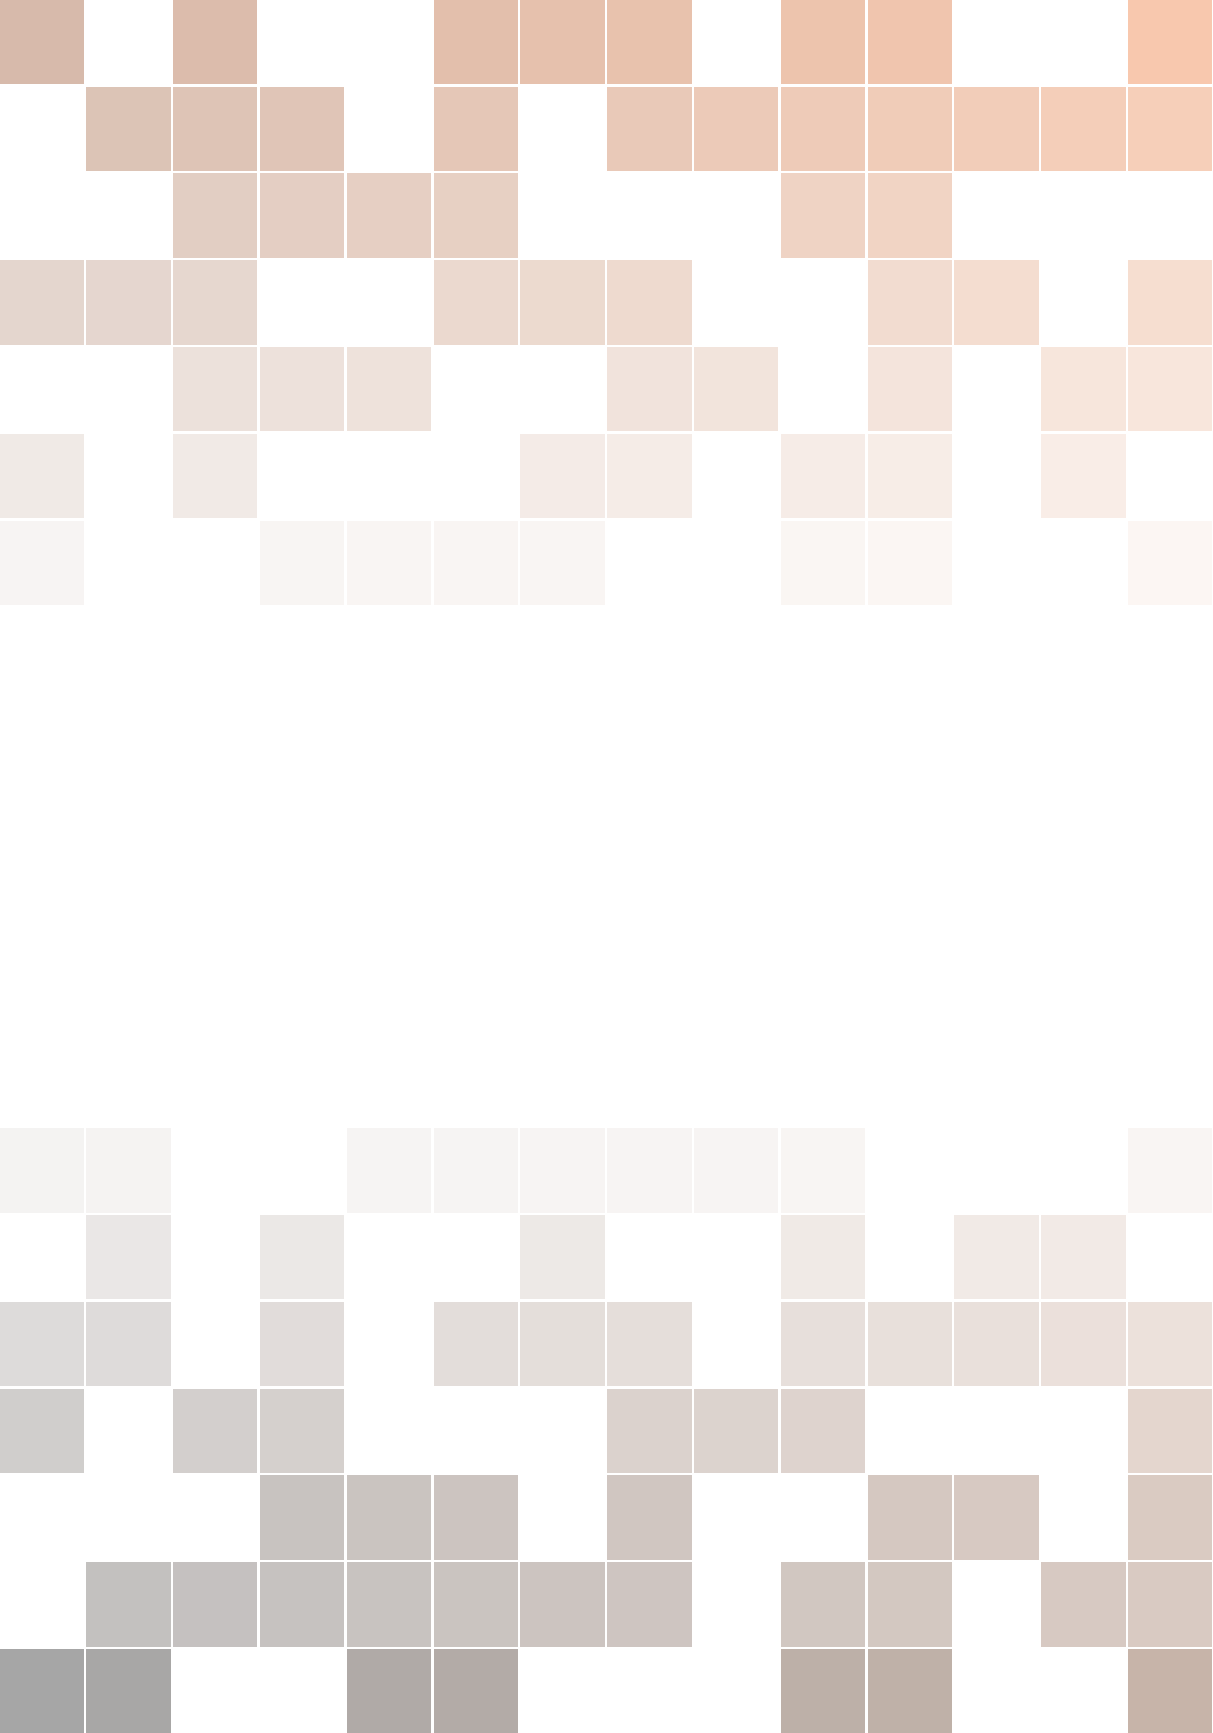
\includegraphics[width=\paperwidth]{background.pdf}};
\draw (current page.center) node [fill=ocre!30!white,fill opacity=0.6,text opacity=1,inner sep=1cm]{\Huge\centering\bfseries\sffamily\parbox[c][][t]{\paperwidth}{\centering \BookName \\[15pt] % Book title
{\Large Сборник статей}\\[20pt] % Subtitle
{\huge \AuthorName}}}; % Author name
\end{tikzpicture}
\vfill
\endgroup

%----------------------------------------------------------------------------------------
%	COPYRIGHT PAGE
%----------------------------------------------------------------------------------------

\newpage
~\vfill
\thispagestyle{empty}

\noindent  \copyright\ 2021 Катехизис Катарсиса\\ % Copyright notice

\noindent \textsc{Опубликовано в Интернете}\\ % Publisher

\noindent \textsc{https://vk.com/catx2}\\ % URL

\noindent Шабллон взят из https://www.latextemplates.com/template/the-legrand-orange-book. Он подчинаяется  Creative Commons Attribution-NonCommercial 3.0 Unported License. \\ % License information, replace this with your own license (if any)

\noindent \textit{First printing, Август 2021} % Printing/edition date

%----------------------------------------------------------------------------------------
%	TABLE OF CONTENTS
%----------------------------------------------------------------------------------------

%\usechapterimagefalse % If you don't want to include a chapter image, use this to toggle images off - it can be enabled later with \usechapterimagetrue

\chapterimage{8391.jpg} % Table of contents heading image

\pagestyle{empty} % Disable headers and footers for the following pages
\label{tablecont}
\tableofcontents % Print the table of contents itself

%\cleardoublepage % Forces the first chapter to start on an odd page so it's on the right side of the book

\pagestyle{fancy} % Enable headers and footers again

%----------------------------------------------------------------------------------------
%	PART
%----------------------------------------------------------------------------------------

%\part{Part One}

%----------------------------------------------------------------------------------------
%	CHAPTER 1
%----------------------------------------------------------------------------------------

\chapterimage{I5Uy9-cwU7g.jpg} % Chapter heading image


\chapter{Была ли Россия отсталой?}

Когда в Российской Империи появились первые пароходы, в Японии царил сёгунат и голод. Когда Россия приступила к созданию броненосного флота, то в Японии только разворачивалась революция Мэйдзи. Почему же Россию считают отсталой? Была ли война проиграна до начала или нет?

Русские создавали флот с нуля дважды. Первый раз – при Петре I, второй раз – в конце XIX в. В первый раз у них было два направления для экспансии и два грозных противника. Во второй раз – соперничество с самыми крупными морскими державами, а еще оборона двух морей и одного океана. Поэтому при оценке сил двух империй речь пойдет, в первую очередь, о кораблях. 

\section{Русский флот: от Крыма до Японии.}

В советской историографии красной нитью шла речь об «отсталости Царской России». При Сталине отношение к отечественной истории отошло от привычного охаивания в духе школы Покровского. Но вот Русско-японскую войну всегда выставляли как образец позора Российской империи и Романовых. После СССР появилась прямо противоположная точка зрения. Так где же истина?

Вторая половина XIX в. – это время индустриализации военного комплекса. Крымская война была последним крупным конфликтом с применением парусного флота (2). После нее стало ясно: главную роль играют технологии.

\begin{figure}[h!tb] 
	\centering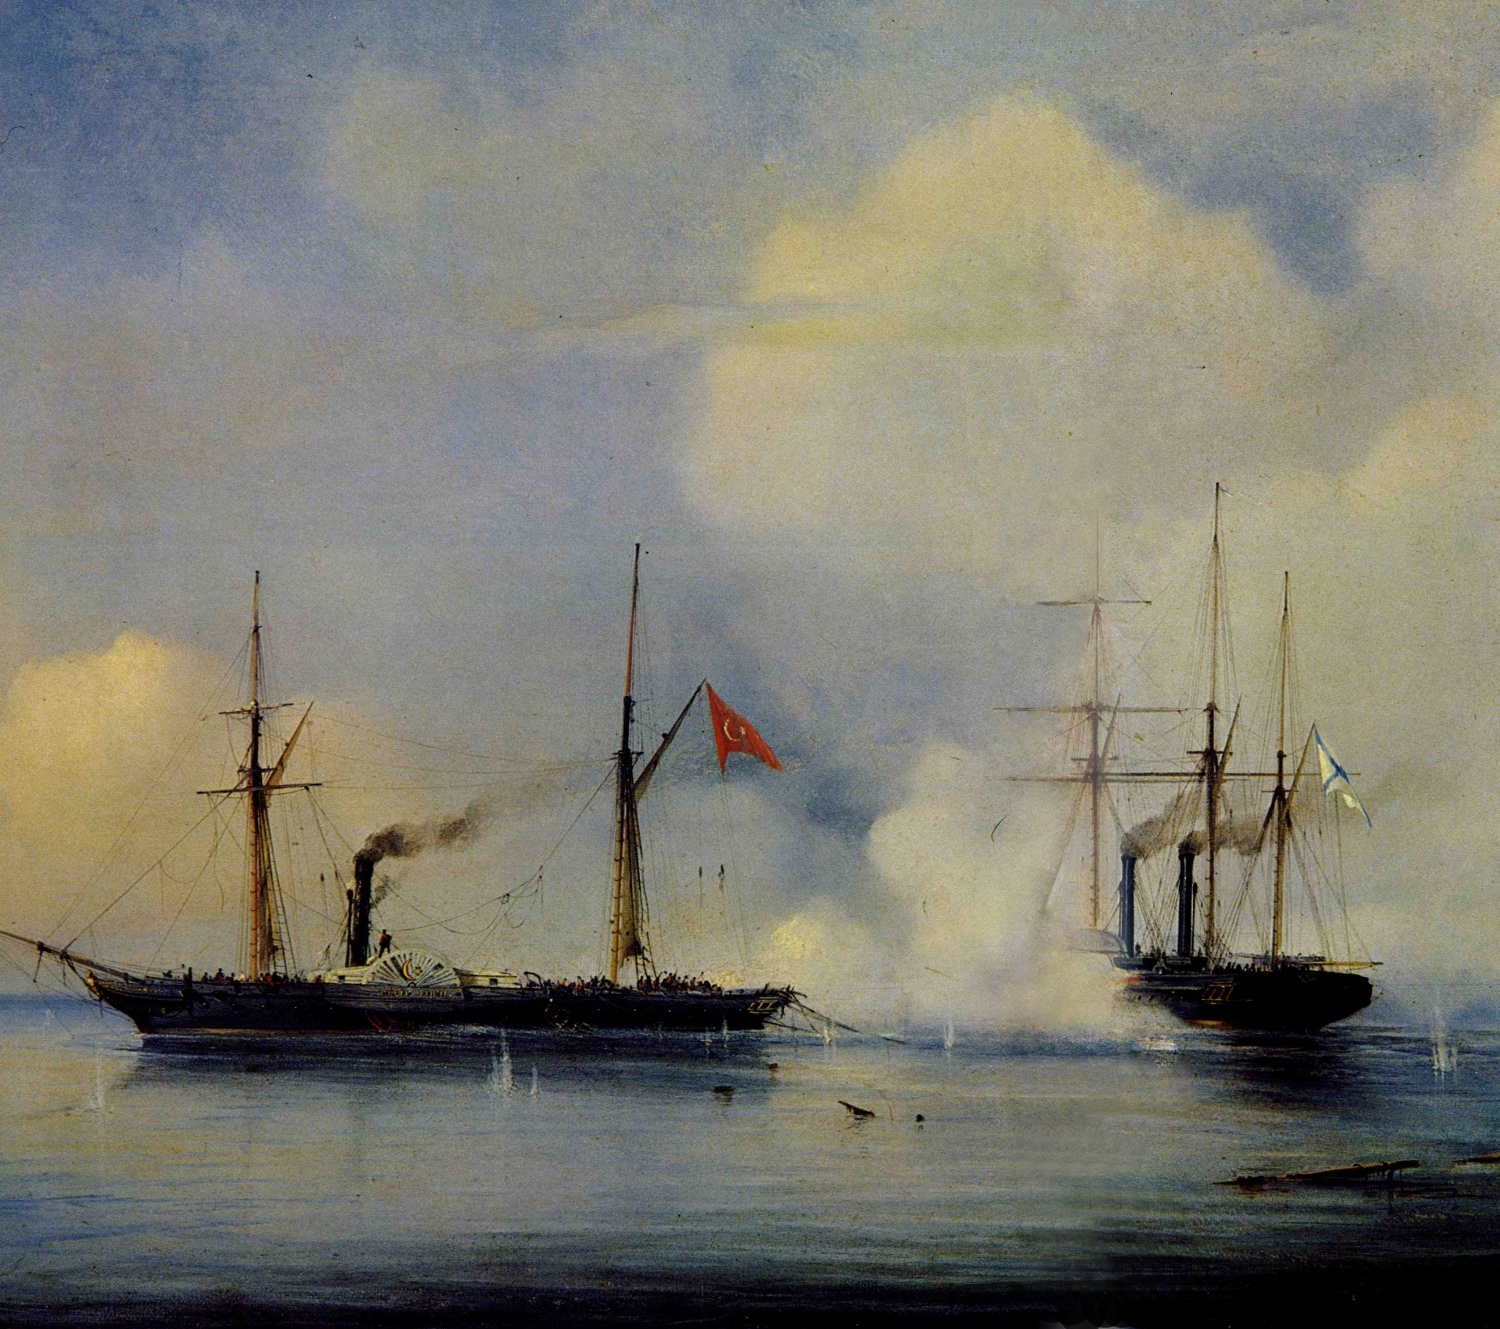
\includegraphics[scale=0.3]{Data/RYAV_sily_storon/rO3nWL7-ijc.jpg}
	%	\label{fig:scipion} % Unique label used for referencing the figure in-text\end{document}
	%	%\addcontentsline{toc}{figure}{Figure \ref{fig:placeholder}} % Uncomment to add the figure to the table of contents%----------------------------------------------------------------------------------------
	\caption{Бой русского пароходофрегата «Владимир» и турецкого парохода «Перваз-Бахри». Художник А. Боголюбов. Это небольшой бой времен Крымской войны стало первым сражением пароходов в истории человечества.}%	CHAPTER 2
\end{figure}

В конце XIX в. вплоть до начала Первой мировой войны в Европейских державах настал период интенсивного военно-промышленного взаимодействия. Военный историк Мак-Нил датирует его с 1884 по 1914 г. На смену фрегатам с белоснежными парусами пришли огромные плавучие броненосцы из стали, проворные катера и подлодки. Торпеды, радио, системы управления огнем стали залогом победы в морских баталиях.

Технологии развивались стремительно. Стратегическая мысль просто не успевала за ним. Прежде адмиралы и министры понимали с ходу каждую инновацию. Теперь же на диалог с изобретателями уходили дни, а на испытания новинок недели и месяцы учений. «Математическая затруднительность проблемы, совершенно явственно превосходившая уровень знаний большинства людей даже из самого узкого круга посвященных, лишала политику минимальной рациональности», – так описывает Мак Нил ситуацию перед Первой Мировой Войной. Эти слова верны и для предшествующих десятилетий.




Назвать Россию отсталой страной сложно хотя бы из-за того, что модернизация флота началась сразу после Крымской Войны. Но и впадать в идеализацию не стоит: завязанная на государство экономика, крепостничество, отсутствие многих отраслей стали препятствиями для создания стальных кораблей. (3)
Не лишним при описании истории Русского флота будет и слово «Геополитика». Кто сильнее: Слон или Кит? Все зависит от среды. Россия не была первой на море, но показала себя неплохой на суше, потопив Наполеона в бескрайних пространствах Восточно-европейской равнины и подплывая через Хартленд Средней Азии к Индии.


Поэтому после Крымской войны о лидерстве на море речь не шла.
\begin{textcitation}
{	
		«Смирившись с невозможностью создать в ближайшее время боевой потенциал флота, равный боевым потенциалам флотов Англии и Франции, и в то же время не желая терять престижа России как одной из крупных морских держав, царское правительство при определении программы нового судостроения исходило из того, что «Россия должна быть первоклассною морскою державою, занимать в Европе третье место по силе флота после Англии и Франции и должна быть сильнее союза второстепенных морских держав» (имелись в виду Пруссия, Швеция и Дания. — Авт.)»}
\end{textcitation} 
пишут В. А. Золотарев и И. А. Козлов в«Трех столетиях Российского флота».\url{http://militera.lib.ru/h/zolotarev_kozlov2/11.html}

\begin{figure}[h!tb] 
	\centering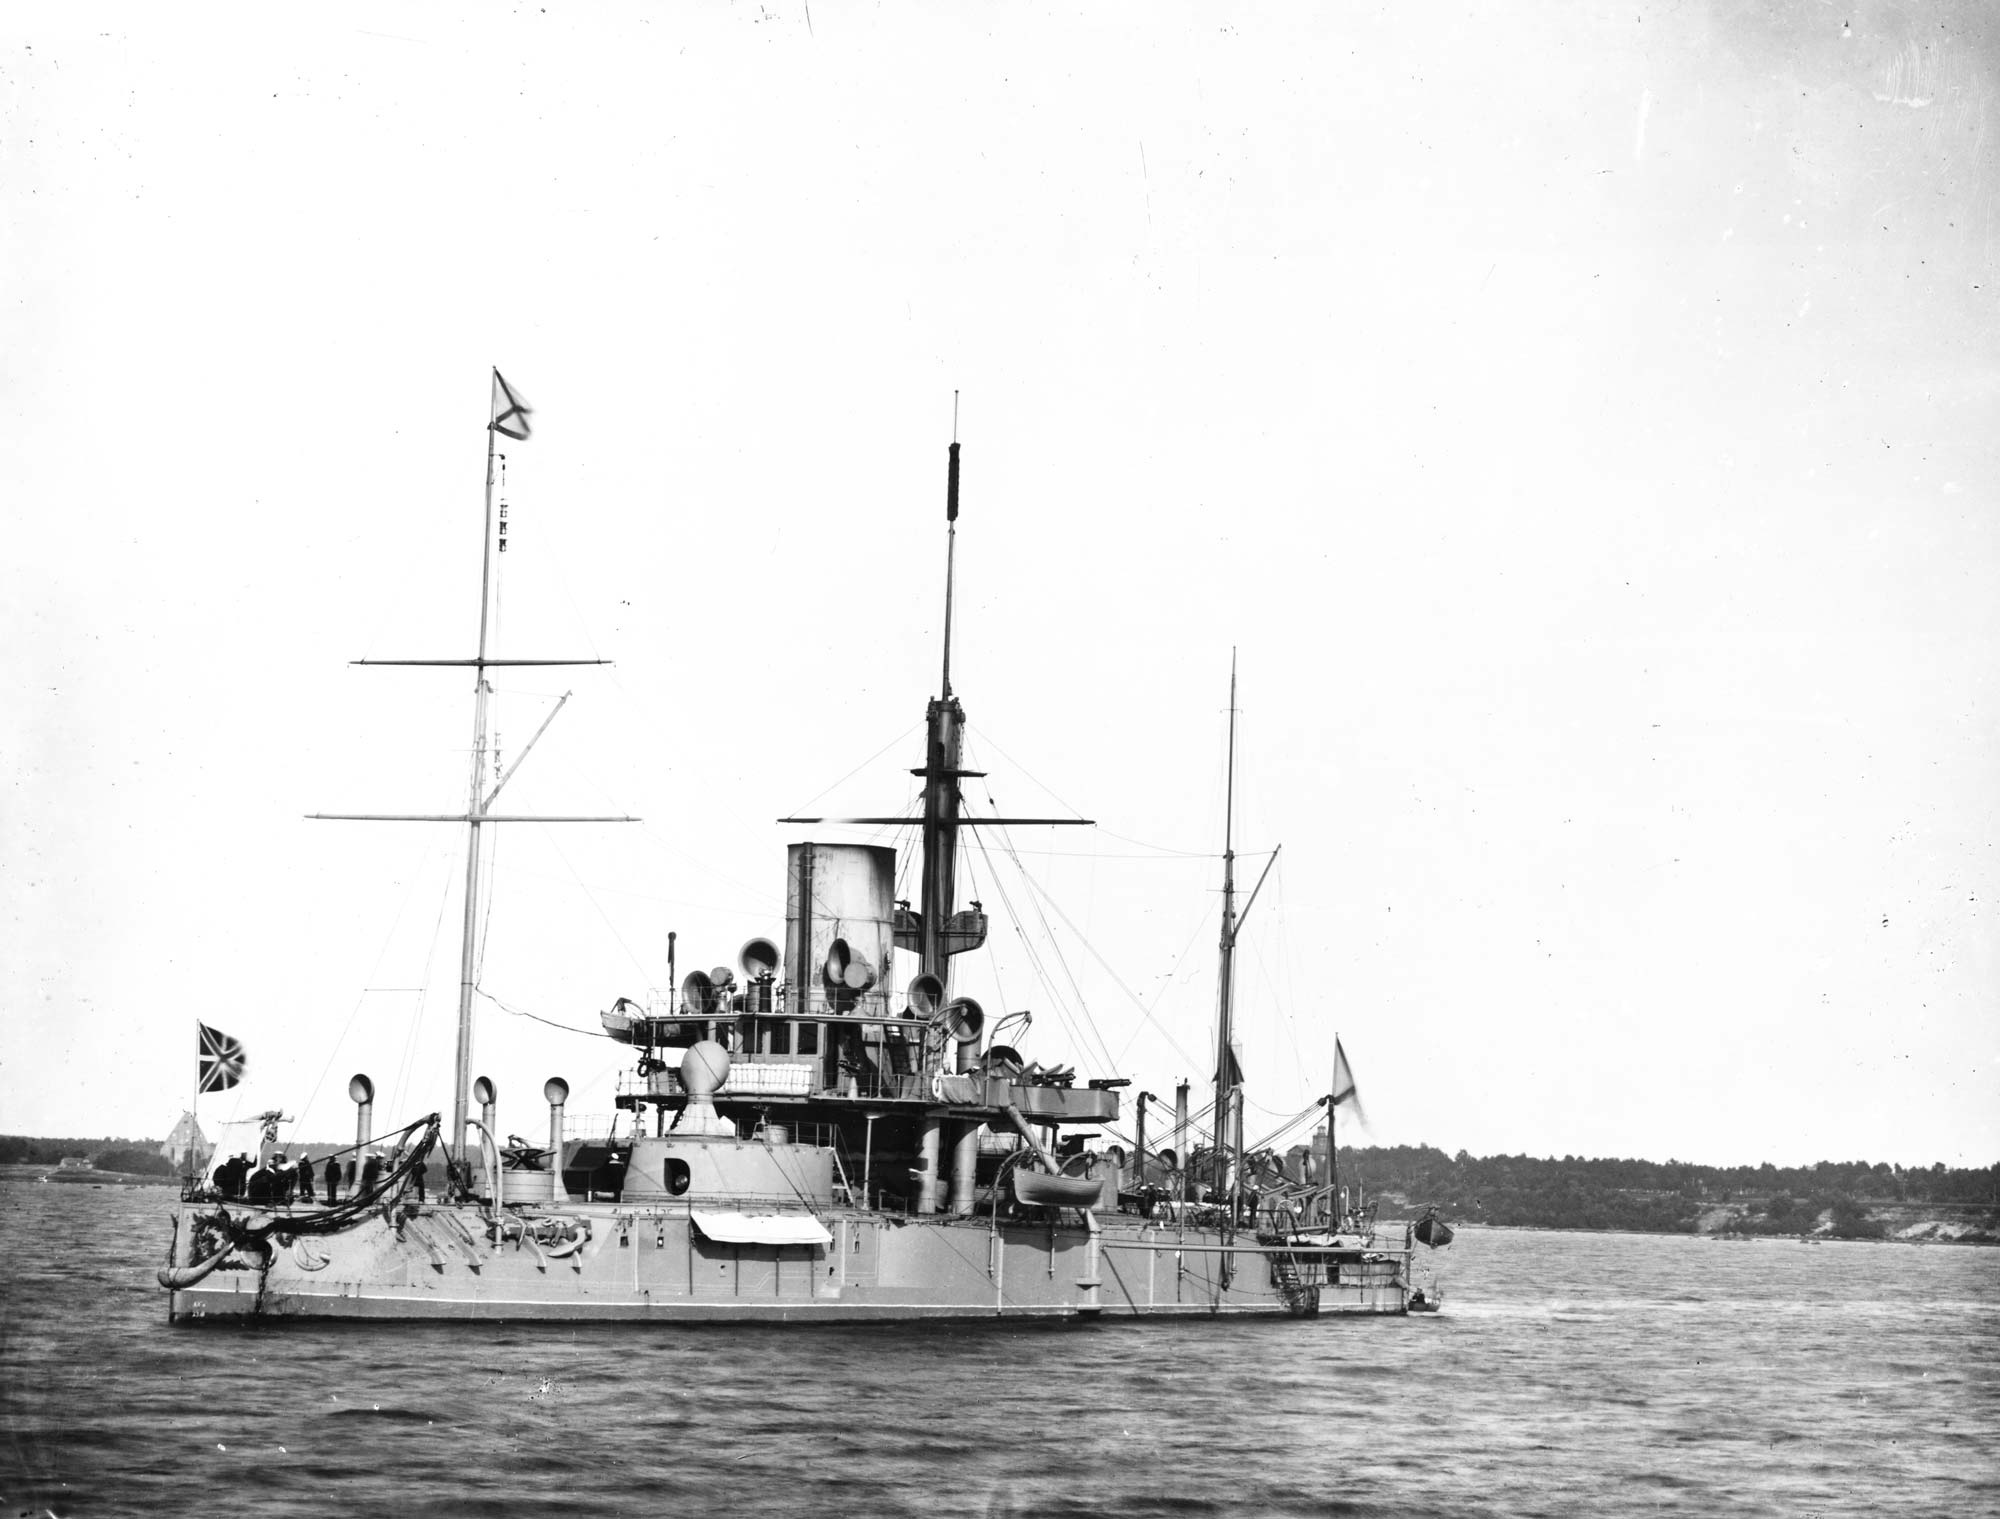
\includegraphics[scale=0.2]{Data/RYAV_sily_storon/jYR7YIwi8uE.jpg}
	%	\label{fig:scipion} % Unique label used for referencing the figure in-text\end{document}
	%	%\addcontentsline{toc}{figure}{Figure \ref{fig:placeholder}} % Uncomment to add the figure to the table of contents%----------------------------------------------------------------------------------------
	\caption{Первый русский броненосец Пётр Великий. Изначально относился к классу Мониторов. Фотографии взяты с сайта «Цусима» \url{http://tsushima.su/petrvelphotoru/} Фото 1}%	CHAPTER 2
\end{figure}


\begin{figure}[h!tb] 
	\centering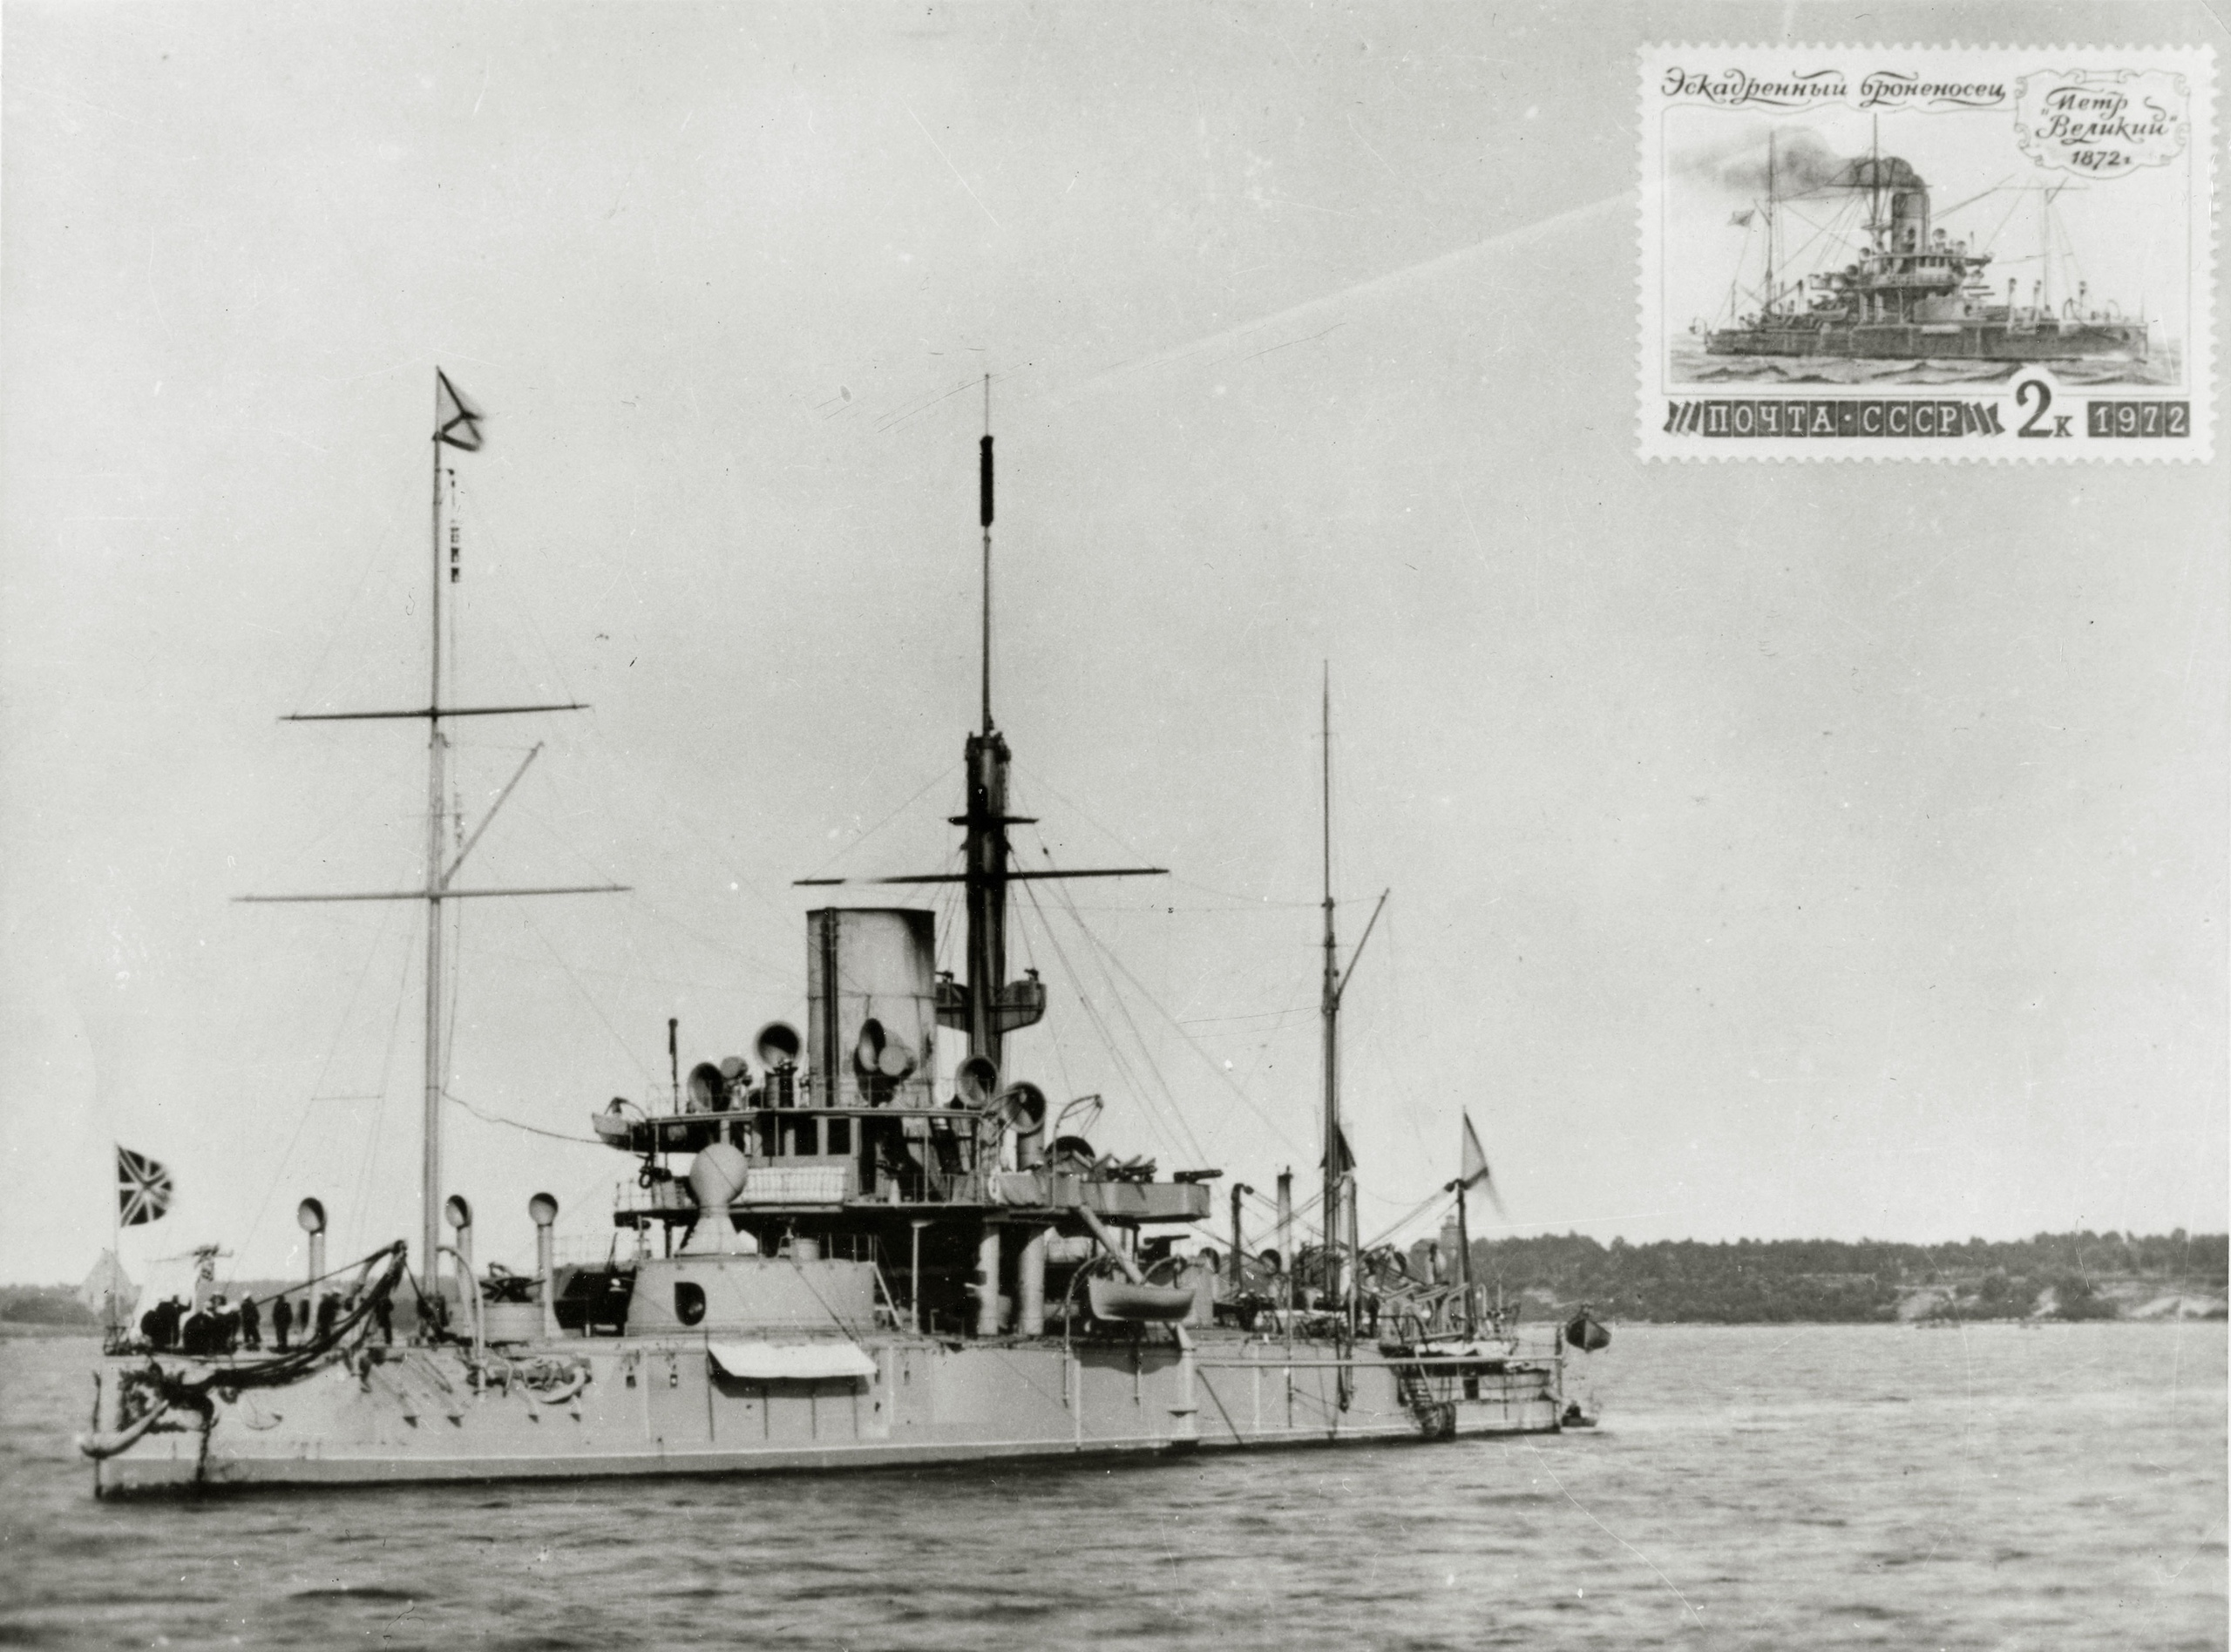
\includegraphics[scale=0.2]{Data/RYAV_sily_storon/wiYS26wh4ZQ.jpg}
	%	\label{fig:scipion} % Unique label used for referencing the figure in-text\end{document}
	%	%\addcontentsline{toc}{figure}{Figure \ref{fig:placeholder}} % Uncomment to add the figure to the table of contents%----------------------------------------------------------------------------------------
	\caption{Первый русский броненосец Пётр Великий. Изначально относился к классу Мониторов. Фотографии взяты с сайта «Цусима» \url{http://tsushima.su/petrvelphotoru/} Фото 2}%	CHAPTER 2
\end{figure}
\begin{figure}[h!tb] 
	\centering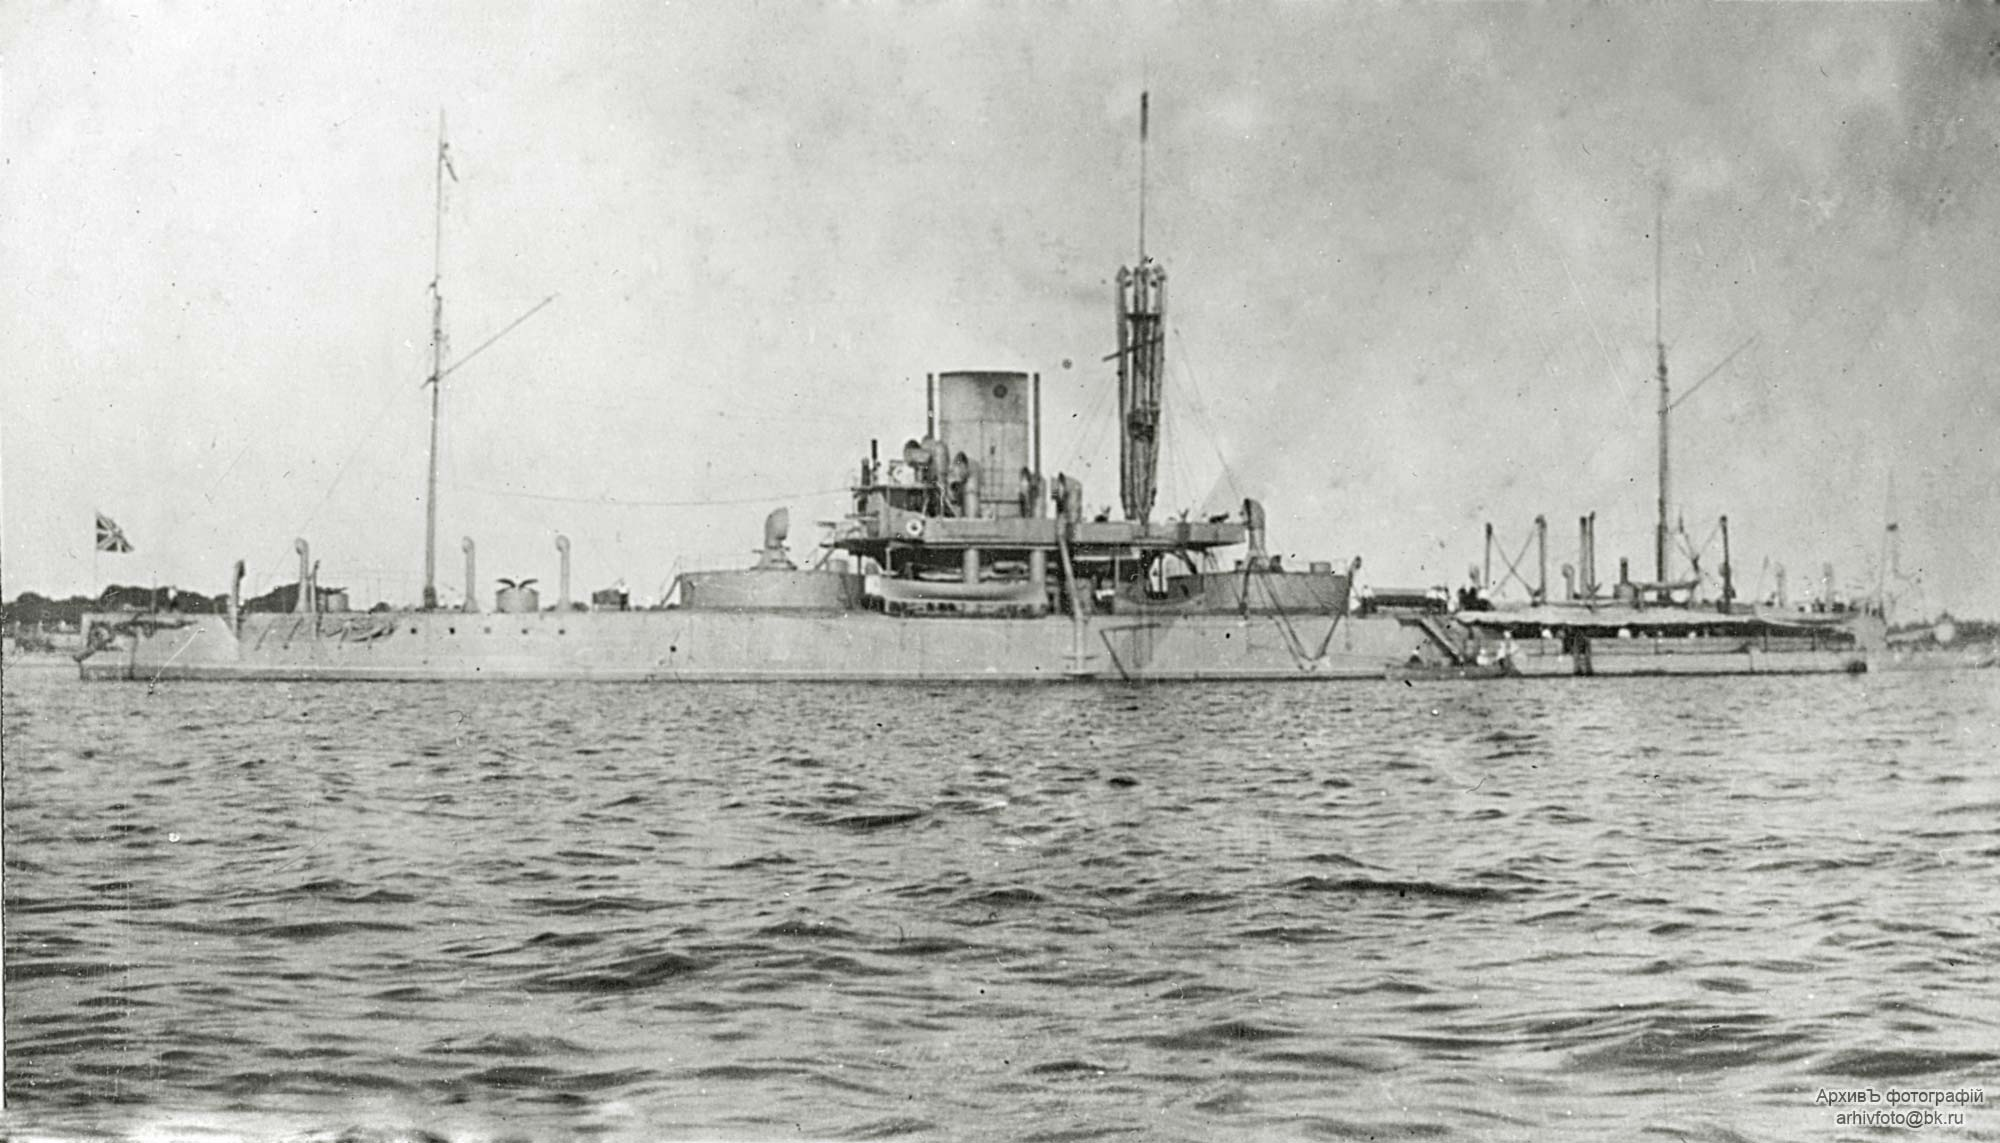
\includegraphics[scale=0.2]{Data/RYAV_sily_storon/dQQjFe6_e2U.jpg}
	%	\label{fig:scipion} % Unique label used for referencing the figure in-text\end{document}
	%	%\addcontentsline{toc}{figure}{Figure \ref{fig:placeholder}} % Uncomment to add the figure to the table of contents%----------------------------------------------------------------------------------------
	\caption{Первый русский броненосец Пётр Великий. Изначально относился к классу Мониторов. Фотографии взяты с сайта «Цусима» \url{http://tsushima.su/petrvelphotoru/} Фото 3}%	CHAPTER 2
\end{figure}

Тем не менее, за 15 лет после Парижского договора на Балтике появился броненосный флот, третий по силе в Европе. Со стапелей сошел и первый полноценный эскадренный броненосец, «Петр Великий». Затем на верфях создали и броненосные крейсеры, быстрые корабли с легкой броней, предназначенные для долгих автономных походов и действий на коммуникациях. Хуже обстояли дела на Черном Море. Южные рубежи решили поначалу охранять «Поповками», огромными круглыми бронированными плавучими крепостями. Они оказались тяжелыми, дорогими и абсолютно бесполезными. Одну такую «тарелку» сделали в Питере и собрали в Николаеве, другую смогли уже построить целиком там. Не всегда развитие технологий идет гладко, как в компьютерной игре от “Парадоксов” или “Цивилизации”. Что и говорить о морской тактике и стратегии. Некоторые светлые умы предлагали даже оснащать корабли таранами и пробивать противника как в античные времена.

\begin{figure}[h!tb] 
	\centering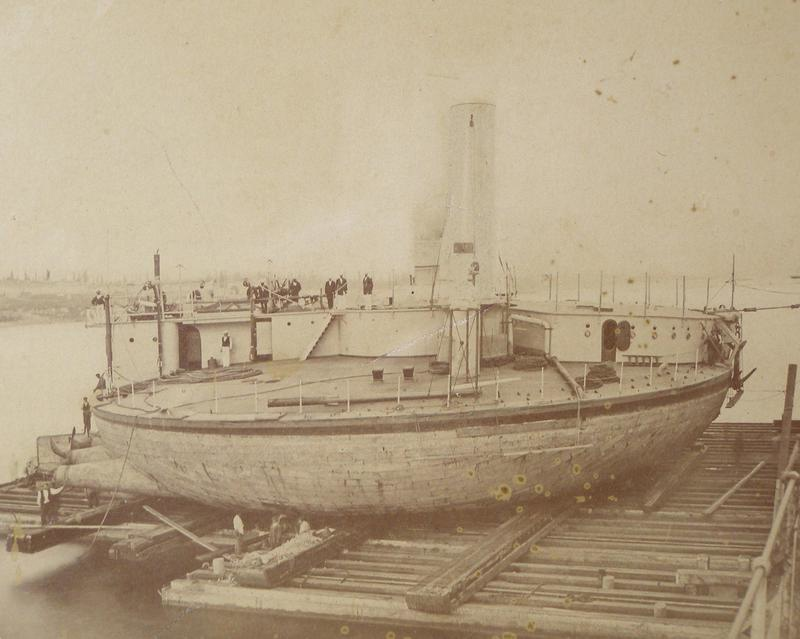
\includegraphics[scale=0.4]{Data/RYAV_sily_storon/GJfhe1Pp85A.jpg}
	%	\label{fig:scipion} % Unique label used for referencing the figure in-text\end{document}
	%	%\addcontentsline{toc}{figure}{Figure \ref{fig:placeholder}} % Uncomment to add the figure to the table of contents%----------------------------------------------------------------------------------------
	\caption{Слабоопознанный плавающий объект «Поповка». Фотография взята с сайта «Поп-механика» \url{https://www.popmech.ru/weapon/13814-plavayushchie-tarelki-absurd/}}%	CHAPTER 2
\end{figure}

В 1880 был принят новый план строительства флота. Мы создавали уже не оборонительно-прибрежный, а океанский. Как видно из таблицы, упор был сделан на Балтику: царское правительство заслуженно опасалось Германской Империи. К тому же Петербург был в то время промышленным центром России.

\begin{figure}[h!tb] 
	\centering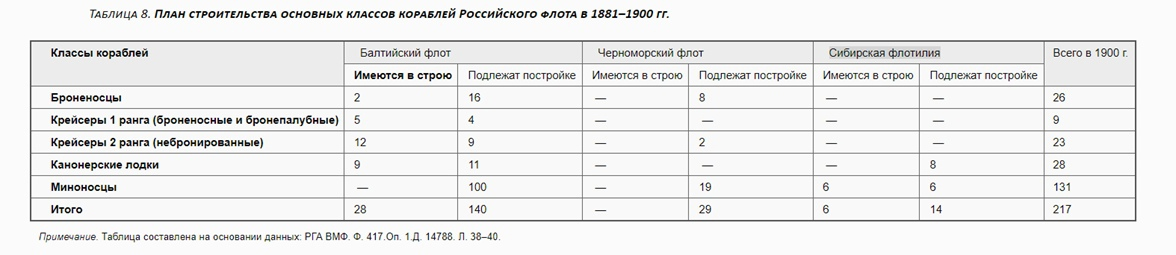
\includegraphics[scale=0.4]{Data/RYAV_sily_storon/eAX9dphs0L4.jpg}
	%	\label{fig:scipion} % Unique label used for referencing the figure in-text\end{document}
	%	%\addcontentsline{toc}{figure}{Figure \ref{fig:placeholder}} % Uncomment to add the figure to the table of contents%----------------------------------------------------------------------------------------
	\caption{Источник: Золотарев В.А., Козлов И.А. Три столетия Российского флота»}%	CHAPTER 2
\end{figure}

В это же время сложилась классификация кораблей флота. Расскажу о ней вкратце (цифры взяты из монографии В. А. Золотарева и И. А. Козлова «Три столетия Российского флота».
1) Эскадренный броненосец или просто броненосец. Огромная плавучая гора с кучей пушек. Минус – неповоротливость. Некоторые же из них, такие как Полтава, еще и не отличались дальностью хода.

\textbf{«Водоизмещение 10–15 тыс. т; вооружение: артиллерийское — четыре 305-мм, до двенадцати 152-мм, до двадцати 75-мм и до тридцати 47–37-мм орудий; торпедное — до четырех надводных и двух подводных торпедных аппаратов; бронирование 406–250 мм; скорость 17–18 узлов; дальность плавания до 8 тыс. миль».}


Первым Броненосцем, если не считать корабль «Петр Первый», был «Император Александр I». Но вплоть до русско-японской войны при постройке вот таких Левиафанов ориентировались на сделанный чуть позже, в 1891 г., «Наварин». В дальнейшем появилось немало броненосцев разных конструкций. Самой многочисленной серией был тип «Бородино».
\begin{textcitation}
«Создание кораблей типа «Бородино» явилось несомненным достижением российской промышленности. Более многочисленные серии броненосцев до этого строились только для британского флота, четыре серии по пять кораблей в каждой в 1895-1907 гг. были построены для флота Германии»,	
\end{textcitation}
подчеркнул Владимир Грибовский про эти суда.\url{http://tsushima.su/RU/libru/i/Page_6/page_15/grib-borodino/}

\begin{figure}[h!tb] 
	\centering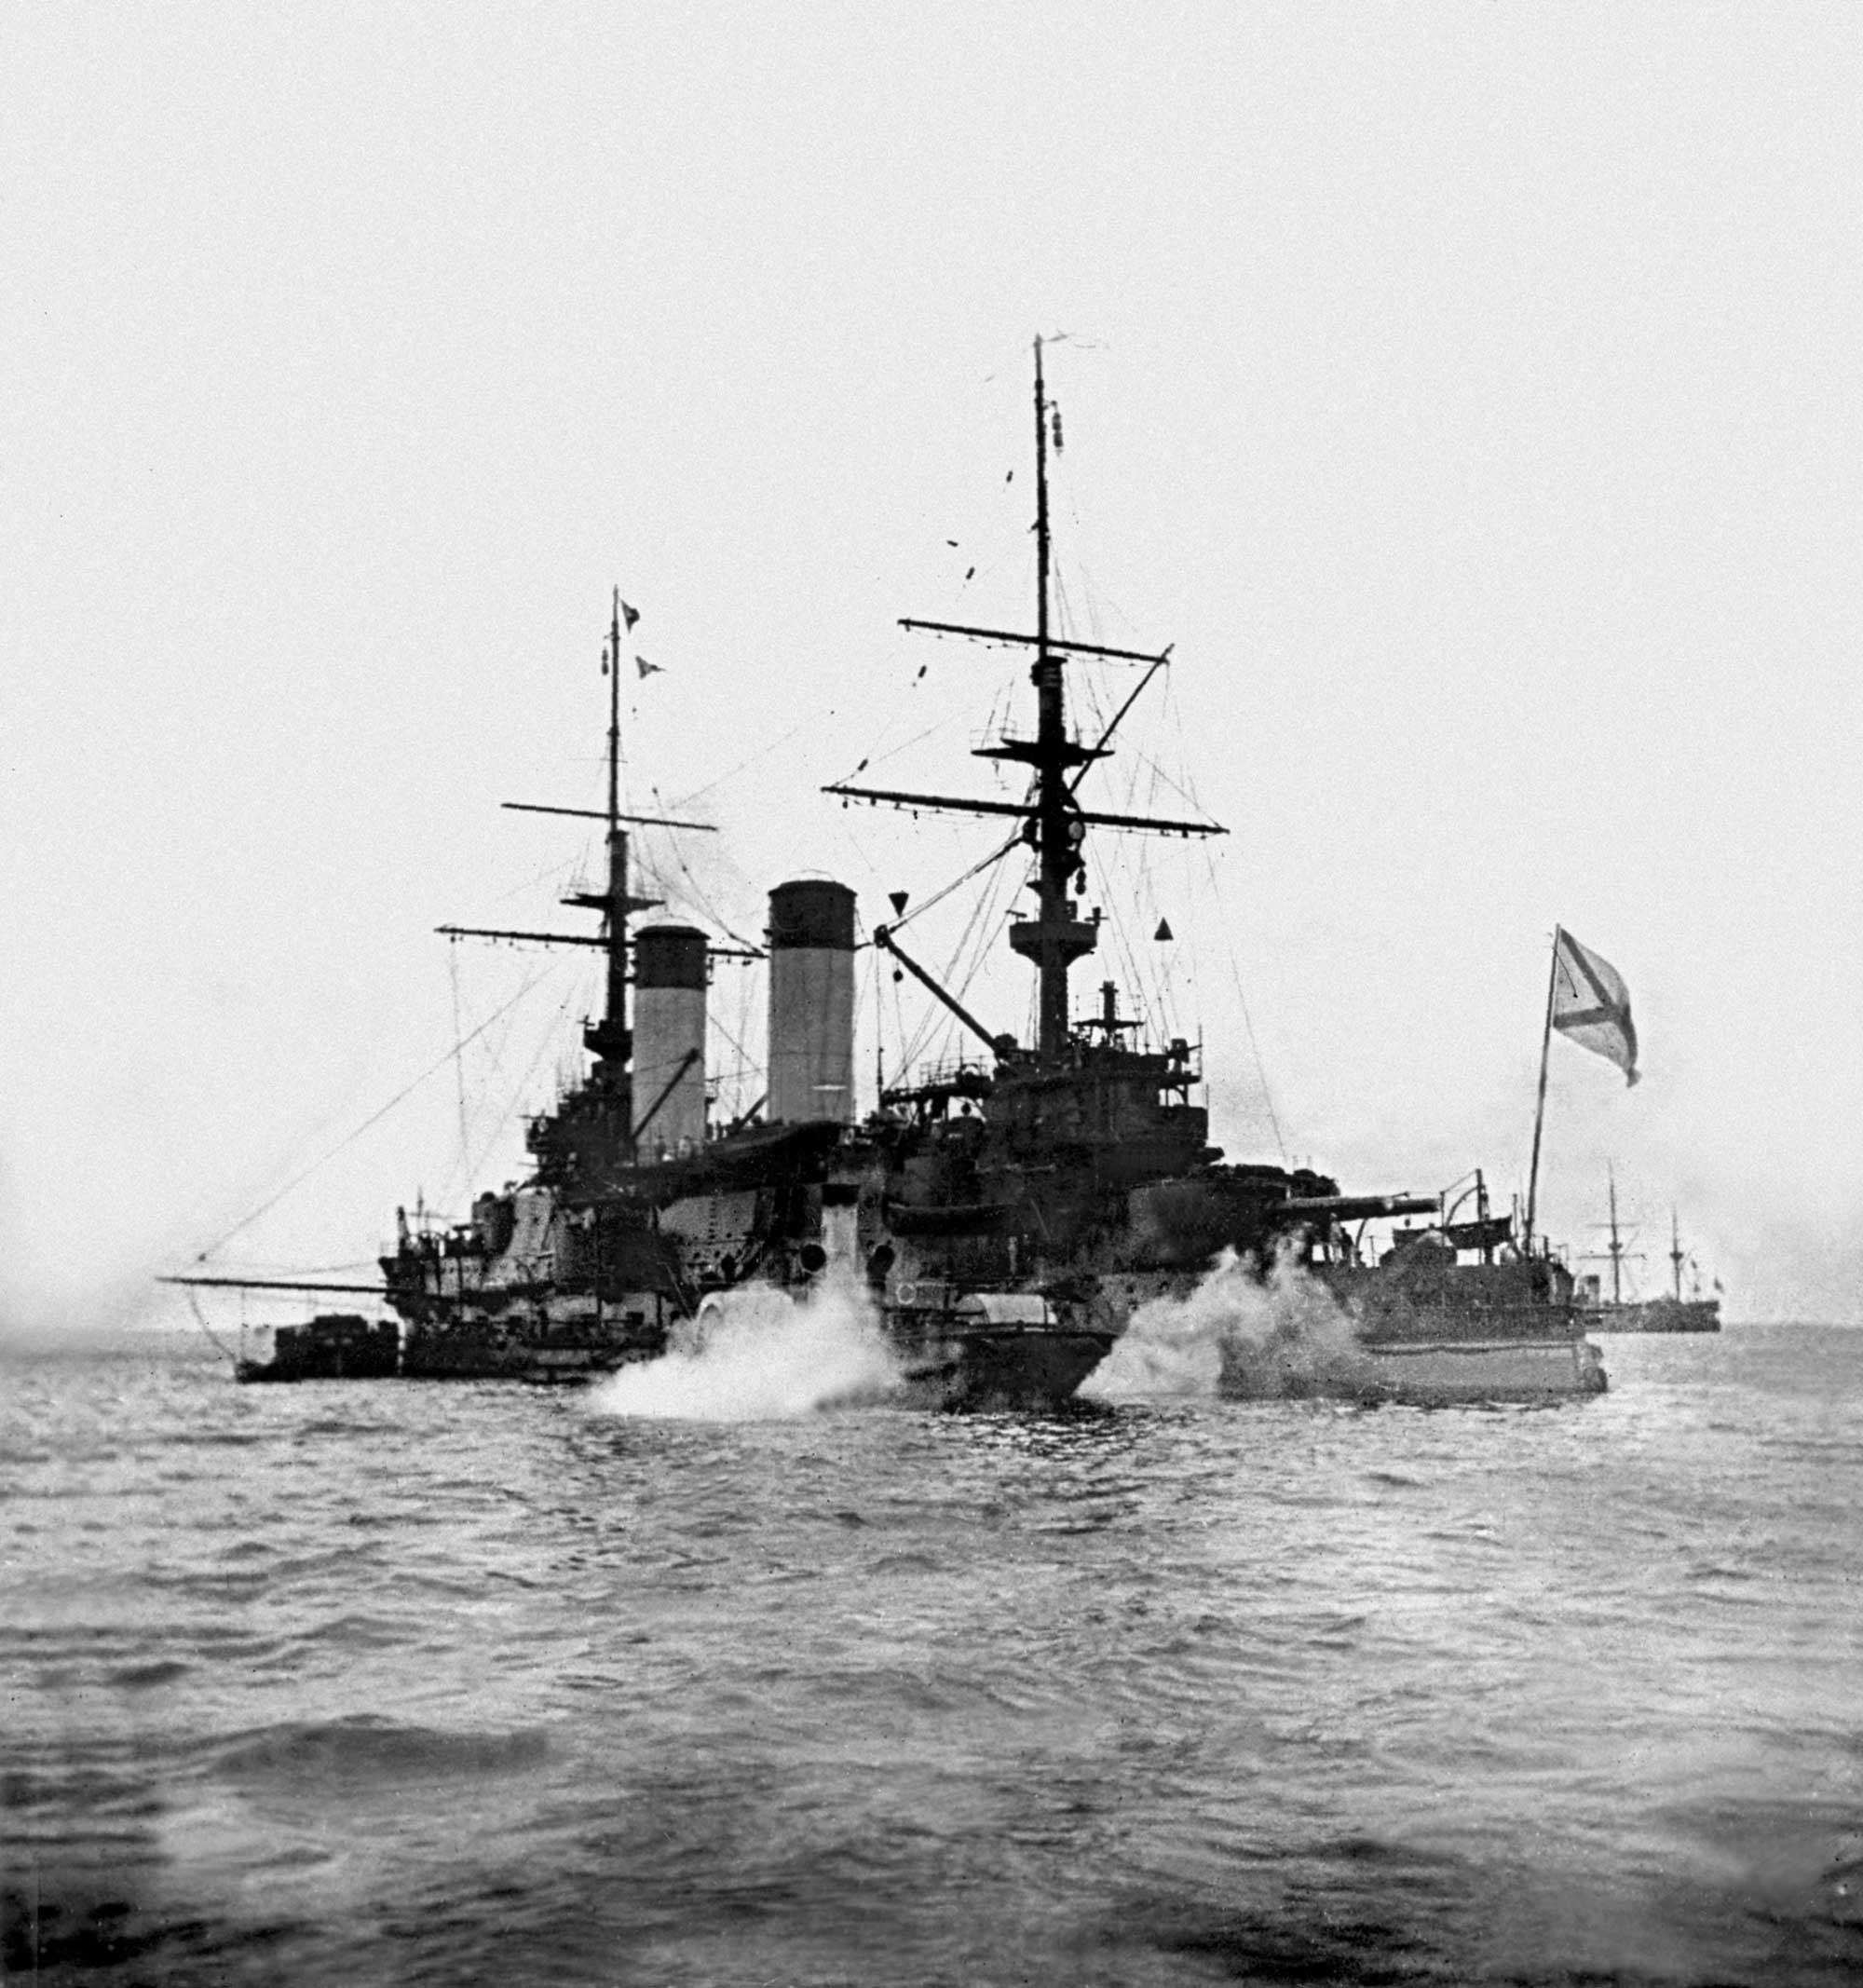
\includegraphics[scale=0.2]{Data/RYAV_sily_storon/pDAKm_tQdIg.jpg}
	%	\label{fig:scipion} % Unique label used for referencing the figure in-text\end{document}
	%	%\addcontentsline{toc}{figure}{Figure \ref{fig:placeholder}} % Uncomment to add the figure to the table of contents%----------------------------------------------------------------------------------------
	\caption{Эскадренный броненосец "Бородино" на малом Кронштадтском рейде. Фотографии взяты с сайта «Цусима»
	}%	CHAPTER 2
\end{figure}


2) Крейсер 1-ого ранга. Проворная плавучая гора с броней, способная как сражаться в эскадре, так и становиться странствующим рыцарем морей, стальной хищной акулой. Самый известный из них – «Аврора» (тип Паллада).

\textbf{«Водоизмещение достигало 12 тыс. т, скорость — 20 узлов, дальность плавания — 8000 миль; вооружение: артиллерийское — четыре 203-мм, шестнадцать 152-мм, до тридцати 37-мм орудий, торпедное — до четырех надводных торпедных аппаратов; бронирование — до 203 мм».}

\begin{figure}[h!tb] 
	\centering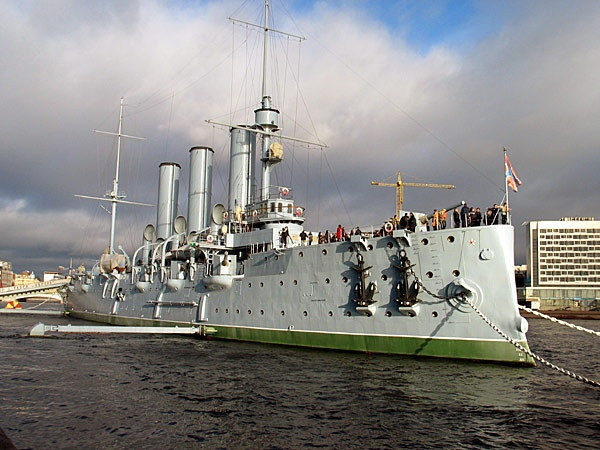
\includegraphics[scale=0.5]{Data/RYAV_sily_storon/o2cXT_E28cA.jpg}
	%	\label{fig:scipion} % Unique label used for referencing the figure in-text\end{document}
	%	%\addcontentsline{toc}{figure}{Figure \ref{fig:placeholder}} % Uncomment to add the figure to the table of contents%----------------------------------------------------------------------------------------
	\caption{«Аврора». Фото с официального сайта \url{http://aurora.org.ru/info/krejser-1-go-ranga-avrora-na-vechnoj-stoyanke-u-petrovskoj-naberezhnoj-sankt-peterburg/}
	}%	CHAPTER 2
\end{figure}

3) Крейсер 2-ого ранга – небольшой корабль для разведки и обороны.

\textbf{«Водоизмещение от 3000 до 6000 т, скорость до 25 узлов, дальность плавания до 4000 миль; вооружение: артиллерийское — восемь 152-мм, двадцать четыре 75-мм, восемь 37-мм орудий; торпедное — до четырех торпедных аппаратов».}

\begin{figure}[h!tb] 
	\centering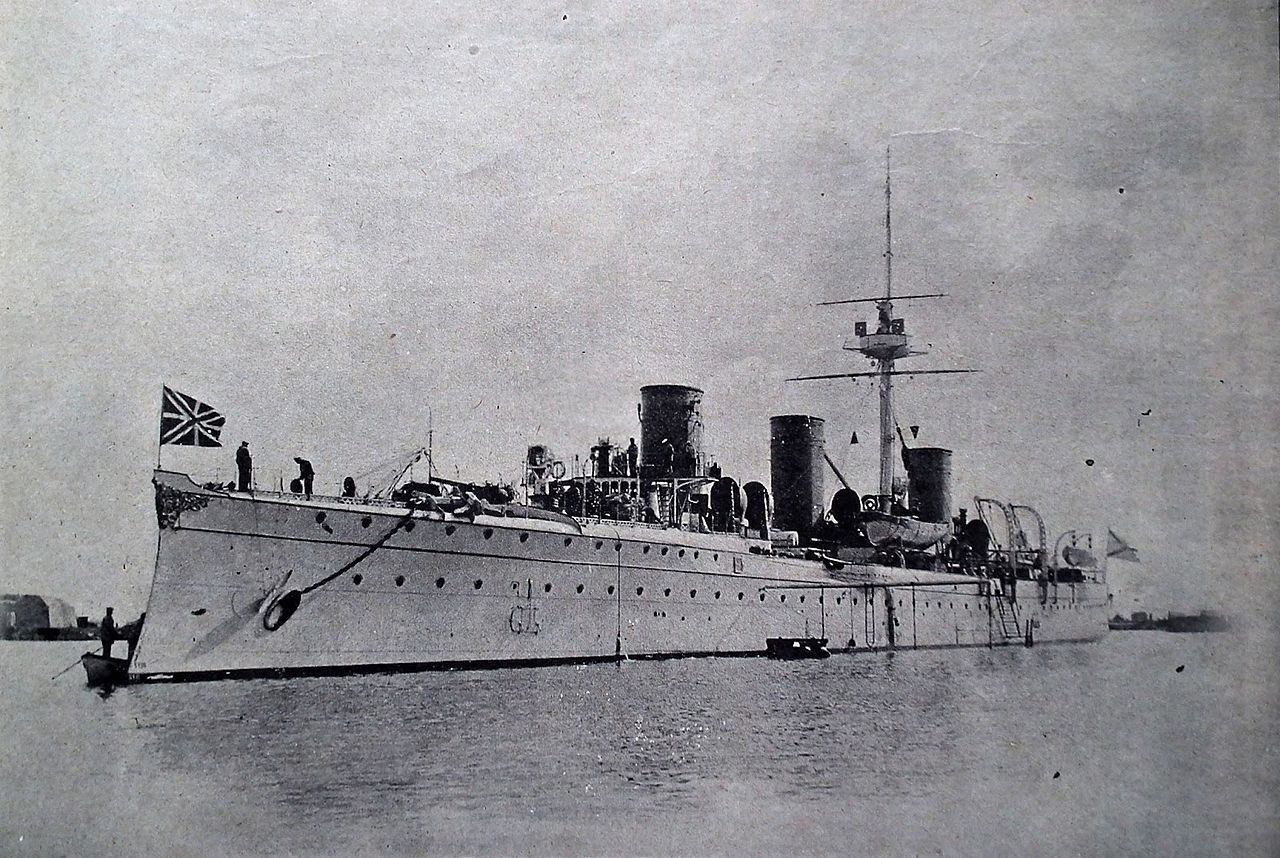
\includegraphics[scale=0.3]{Data/RYAV_sily_storon/f7G2P9E6i0c.jpg}
	%	\label{fig:scipion} % Unique label used for referencing the figure in-text\end{document}
	%	%\addcontentsline{toc}{figure}{Figure \ref{fig:placeholder}} % Uncomment to add the figure to the table of contents%----------------------------------------------------------------------------------------
	\caption{Крейсер II ранга «Новик» }
	%	CHAPTER 2
\end{figure}

4) Канонерская лодка. Небольшое судно, чтоб бить врага вблизи берега.

\textbf{«Водоизмещение до 1500 т, скорость до 15 узлов и по два орудия калибром от 152 до 225 мм».}

\begin{figure}[h!tb] 
	\centering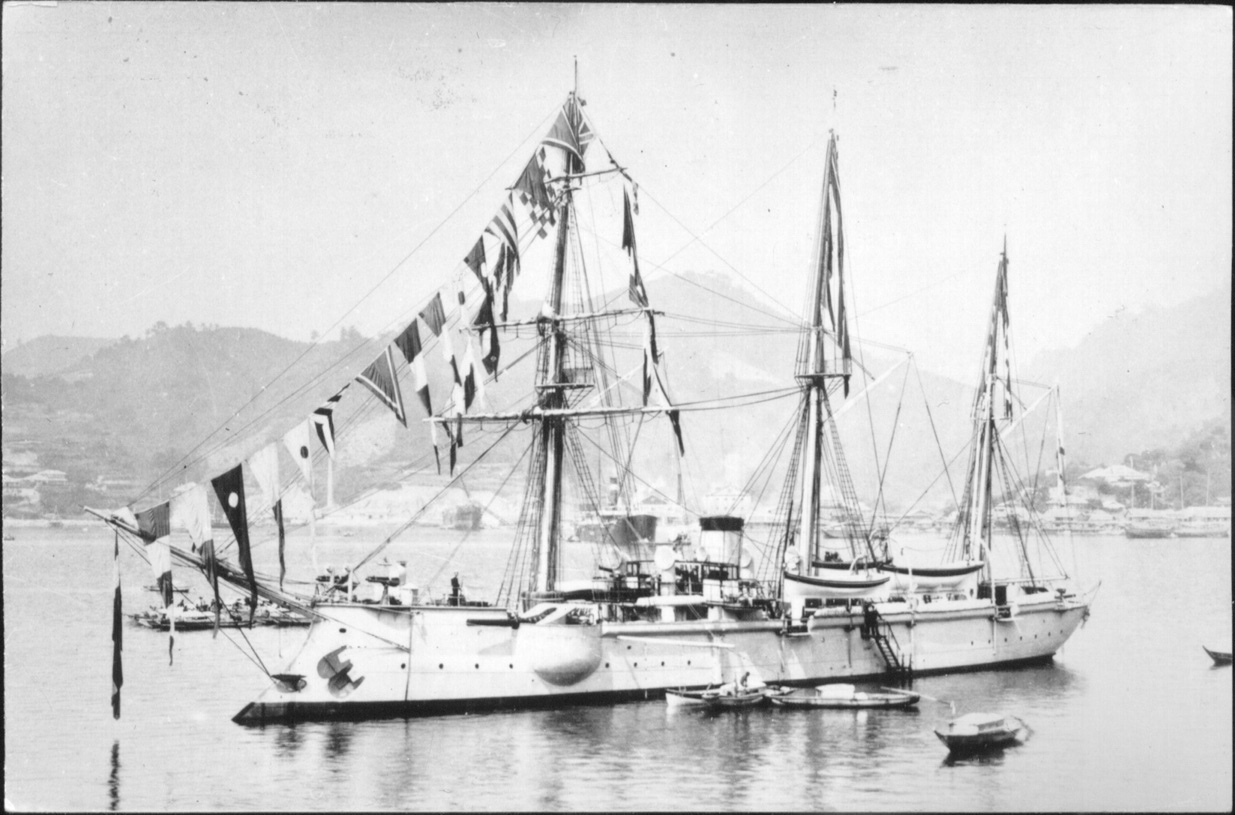
\includegraphics[scale=0.3]{Data/RYAV_sily_storon/7qe4VyVHQn0.jpg}
	%	\label{fig:scipion} % Unique label used for referencing the figure in-text\end{document}
	%	%\addcontentsline{toc}{figure}{Figure \ref{fig:placeholder}} % Uncomment to add the figure to the table of contents%----------------------------------------------------------------------------------------
	\caption{Канонерская лодка «Кореец»
	 }
%	CHAPTER 2
\end{figure}

5) Миноносец и эскадренный миноносец. Маленький, но злой кораблик с торпедами.

\textbf{«Водоизмещение эскадренных миноносцев до 350 т, скорость до 27 узлов, одно 75-мм и пять 47-мм орудий, три торпедных аппарата; у миноносцев водоизмещение до 180 т, скорость до 24 уз., три 37-мм орудия, два торпедных аппарата».}

\begin{figure}[h!tb] 
	\centering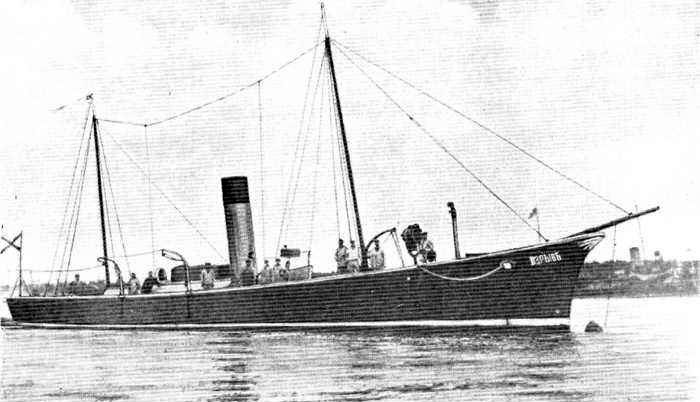
\includegraphics[scale=0.4]{Data/RYAV_sily_storon/a1QM7sSGutc.jpg}
	%	\label{fig:scipion} % Unique label used for referencing the figure in-text\end{document}
	%	%\addcontentsline{toc}{figure}{Figure \ref{fig:placeholder}} % Uncomment to add the figure to the table of contents%----------------------------------------------------------------------------------------
	\caption{Миноносец «Взрыв»
	}
	%	CHAPTER 2
\end{figure}

6) Минный транспорт. Штука, ставящая мины.

\textbf{«Водоизмещение достигало 2800 т, скорость — до 17 узлов, вооружение состояло из пяти 75-мм и семи 47-мм орудий; могли принимать до 300–400 мин».}

\begin{figure}[h!tb] 
	\centering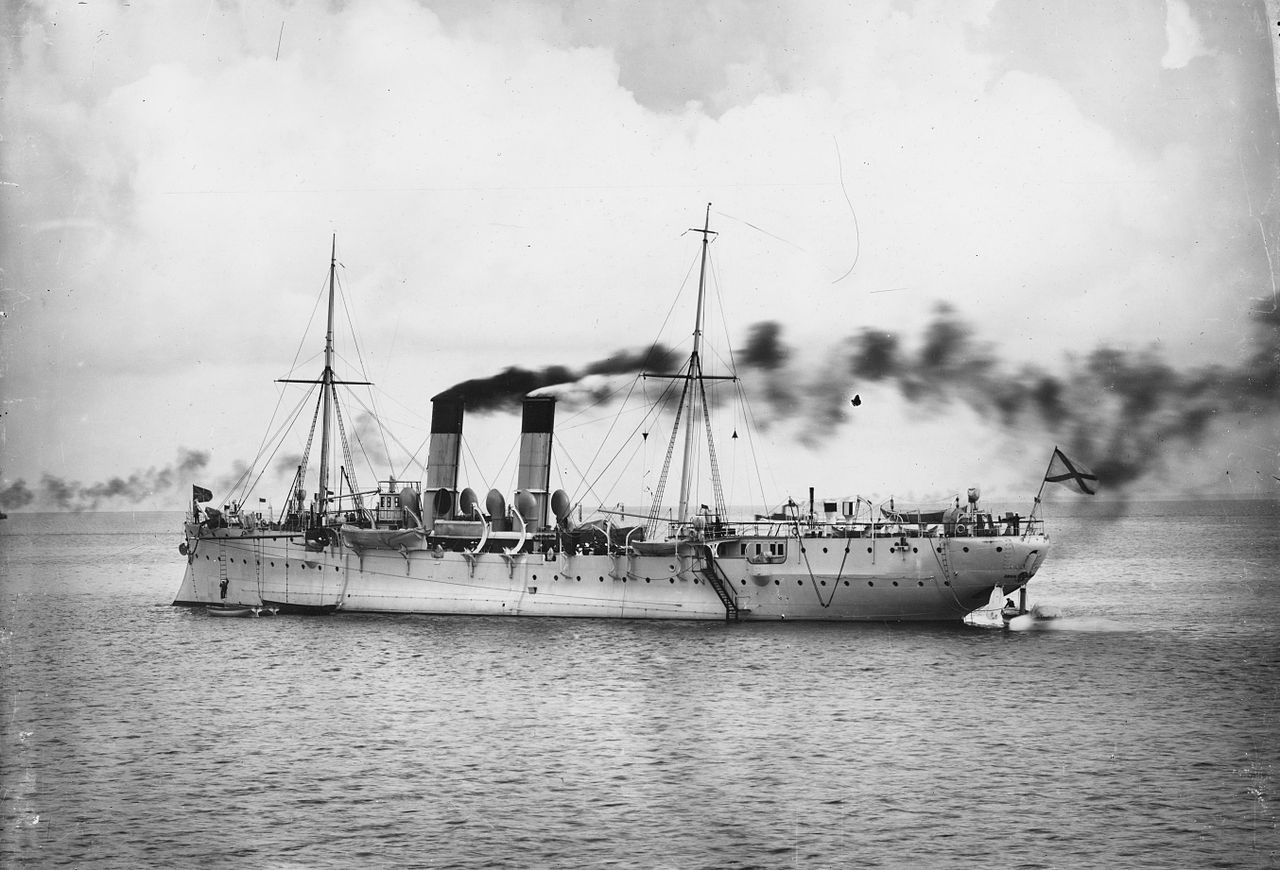
\includegraphics[scale=0.3]{Data/RYAV_sily_storon/w5qmReYSZTc.jpg}
	%	\label{fig:scipion} % Unique label used for referencing the figure in-text\end{document}
	%	%\addcontentsline{toc}{figure}{Figure \ref{fig:placeholder}} % Uncomment to add the figure to the table of contents%----------------------------------------------------------------------------------------
	\caption{Минный заградитель «Амур»
	}
	%	CHAPTER 2
\end{figure}

В 80-х гг начался новый этап строительства флота. В 90-е гг. русский изобретатель А. П. Давыдов создал систему автоматического управления огнем. В тоже время появилась никелированная сталь, радиосвязь и торпеды. «К началу русско-японской войны на вооружении [472] русского флота имелись 45-см торпеды, снабженные гироскопическим прибором управления движением торпеды по направлению, с дальностью хода 2000 м (при скорости 36 узлов) и 1000 м (при скорости 32 узла)».
С другой же стороны, немалая доля «начинки» для тех же кораблей была иностранного производства.
\begin{textcitation}
«При подготовке к походу на «Бородино» были установлены оптические прицелы системы Перепелкина для орудий калибром от 75 до 305 мм, два дальномера системы Барра и Струда, станция беспроволочного телеграфирования системы "Сляби-Арко" германской фирмы "Телефункен", стрелы Темперлея и устройства Спенсера-Миллера для погрузки угля»
\end{textcitation}
 пишет В. Ю. Грибовский в работе об эскадренном броненосце Бородино.

Но такая практика не была редкостью и на Западе. Например, итальянские крейсера типа «Джузеппе Гарибальди» оснащались британской артиллерией фирмы Армстронг. Японские корабли «Касуга» и «Нисима», сделанные на их основе, также несли английские пушки. Работ, подсчитывающих точное соотношение отечественных и западных устройств и оружий, а также технологий, я не нашел.
Благодаря военной реформе Милютина, флот комплектовался не через рекрутские наборы, а ВСЕСОСЛОВНУЮ повинность. Модернизировались и военно-морские училища.
Но почему далеко не худший флот мира проиграл стране, которая в 1850 гг. находилась в состоянии средневековья?

\section{Сравнение Русского и Японского флота}

В целом, русский флот превосходил японский. Но он оказывался распылен на трех направлениях: Тихий Океан, Балтика и Черное море. Проливы и северные воды тревожили Царское правительство, это становится ясно из прошлой статьи про дипломатию. Не выветрилась из памяти и русско-турецкая война 1877-1878 гг.
Но и Дальний восток не уходил из внимания чиновников. Программа по тихоокеанскому флоту была пересмотрена. Готовились резервные эскадры и специальная программа для Дальнего Востока.
\begin{textcitation}
 «Предусматривалось построить (сверх программы 1895 г.) 5 эскадренных броненосцев, 16 крейсеров, 2 минных заградителя и 36 эскадренных миноносцев и миноносцев. Выполнение этой программы должно было закончиться в 1905 г.»
\end{textcitation}
пишут В. А. Золотарев и И. А. Козлов. Именно в это время часть кораблей заказали за границей.
Это привело к тому, что “двуглавый орел” буквально метался с одного конца Евразии на другой. Одни высшие чиновники считали, что приоритет должен остаться за Востоком. Другие, что за Западом.

\begin{textcitation}
«В состав русской эскадры на Тихом океане входили 7 эскадренных броненосцев, 4 броненосных крейсера 1-го ранга, 5 бронепалубных крейсеров 1-го ранга, 2 крейсера 2-го ранга, 6 канонерских лодок, 25 эскадренных миноносцев, 10 миноносцев, 2 минных крейсера, 2 минных заградителя. 1 эскадренный броненосец, 2 крейсера 1-го ранга 1 крейсер 2-го ранга, 7 эскадренных миноносцев, 4 миноносца и 3 транспорта находились в пути на Дальний Восток под командованием вице-адмирала А.А. Вирениуса»
\end{textcitation}
 подытоживает О. Р. Айрапетов.

Против него встал японский флот. 6 новейших эскадренных броненосцев и 6 бронированных крейсеров, т.н. флот «6 на 6». Кроме того, у японцев имелось 6 броненосцев береговой обороны, 7 крейсеров 1-го ранга, 11 крейсеров 2-го ранга, 8 канонерских лодок, 4 минных крейсера и 47 миноносцев. Одновременно, из Средиземного моря в Японию шли 2 броненосных крейсера, купленные в Италии. Таким образом, японцы получили превосходство в ударных силах.

Превосходили ли японские корабли наши? Да.
\begin{textcitation}
 «Три русских броненосца — «Петропавловск», «Севастополь» и «Полтава» являлись уже устаревшими кораблями. <…>. Известный справочник Джейна за 1904 г. соотносил их боевую силу как 0,8 к 1,0 в пользу последних. Кроме того, машины «Севастополя», изготовленные Франко-Русским заводом в Петербурге, отличались низким качеством изготовления и сборки. Даже на официальных испытаниях в 1900 году «Севастополь» не смог развить контрактной скорости (16 узлов), а к началу военных действий с трудом развивал 14» \url{https://cmboat.ru/rusmin1/minonosec3/}
\end{textcitation}
пишет С. В. Несолёный в книге Миноносцы Первой эскадры флота Тихого океана в русско-японской войне (1904-1905 гг.)

И самый главный фактор заключался в том, что Императорский флот Японии превосходил русский в типизации. 
\begin{textcitation}
«Японские эскадренные броненосцы являлись однотипными кораблями новейшей постройки, тогда как русские эскадренные броненосцы, построенные по различным судостроительным программам с интервалом времени до семи лет, принадлежали к четырем различным типам кораблей, обладавшим различными тактико-техническими данными»
\end{textcitation}
продолжает С. В. Несоленый. Да, это не было каким-то сильным превосходством, какое было, например, у регулярной армии над ополчением. Но все равно это дало японцам преимущества. Например, выигрыш в скорости. Русские броненосцы шли медленней на два узла.

При этом японские корабли закупались на Западе. Все броненосцы и практически все броненосные крейсеры сходили на воду с верфей Британии. Большая часть русских судов создавалась – пусть и по западным лекалам – у нас.

И здесь мы отойдем от строго научной литературы в область публицистики. Блогер Половинкин Дмитрий Сергеевич (ЖЖ-юзер Олд-Адмирал) выполнил любительское (но очень качественное) исследование японского флота на основе нескольких научных монографий. Приведу два тезиса.

Японские броненосцы «Сикисима», «Хацусе», «Асахи» и «Микаса» не уступали по своим характеристикам крупнейшим английским кораблям. А вместе эта четверка могла бы набить морду и одному (!) из британских флотов.

Японские броненосные крейсера же имели перекос в сторону боевой мощи, жертвуя остальными параметрами. Такими же характеристиками обладали и вышеупомянутые итальянские корабли Касуга и Нисима. И страна Восходящего Солнца могла себе позволить, так как их противники находились неподалеку. Русские же верфи и промышленные центры располагались на другом конце земного шара. (!)

\begin{textcitation}
«Таким образом, как мы с вами могли убедиться, практически весь японский флот был создан на верфях ведущих кораблестроительных держав. В основном Англии. Выбирались только лучшие проекты и адаптировались под нужные требования. Ядро флота составляли новейшие корабли, характеристики которых в наибольшей степени подходили именно для той войны и того противника, которые выбрала сама Япония. Зачастую это были сильнейшие в мире корабли того времени. Или же превосходство в боевой мощи было достигнуто за счет отказа от тех характеристик, которыми в сложившихся условиях можно было пренебречь» \url{https://oldadmiral.livejournal.com/37890.html}
\end{textcitation}
пишет Олд-Адмирал.

\begin{figure}[h!tb] 
	\centering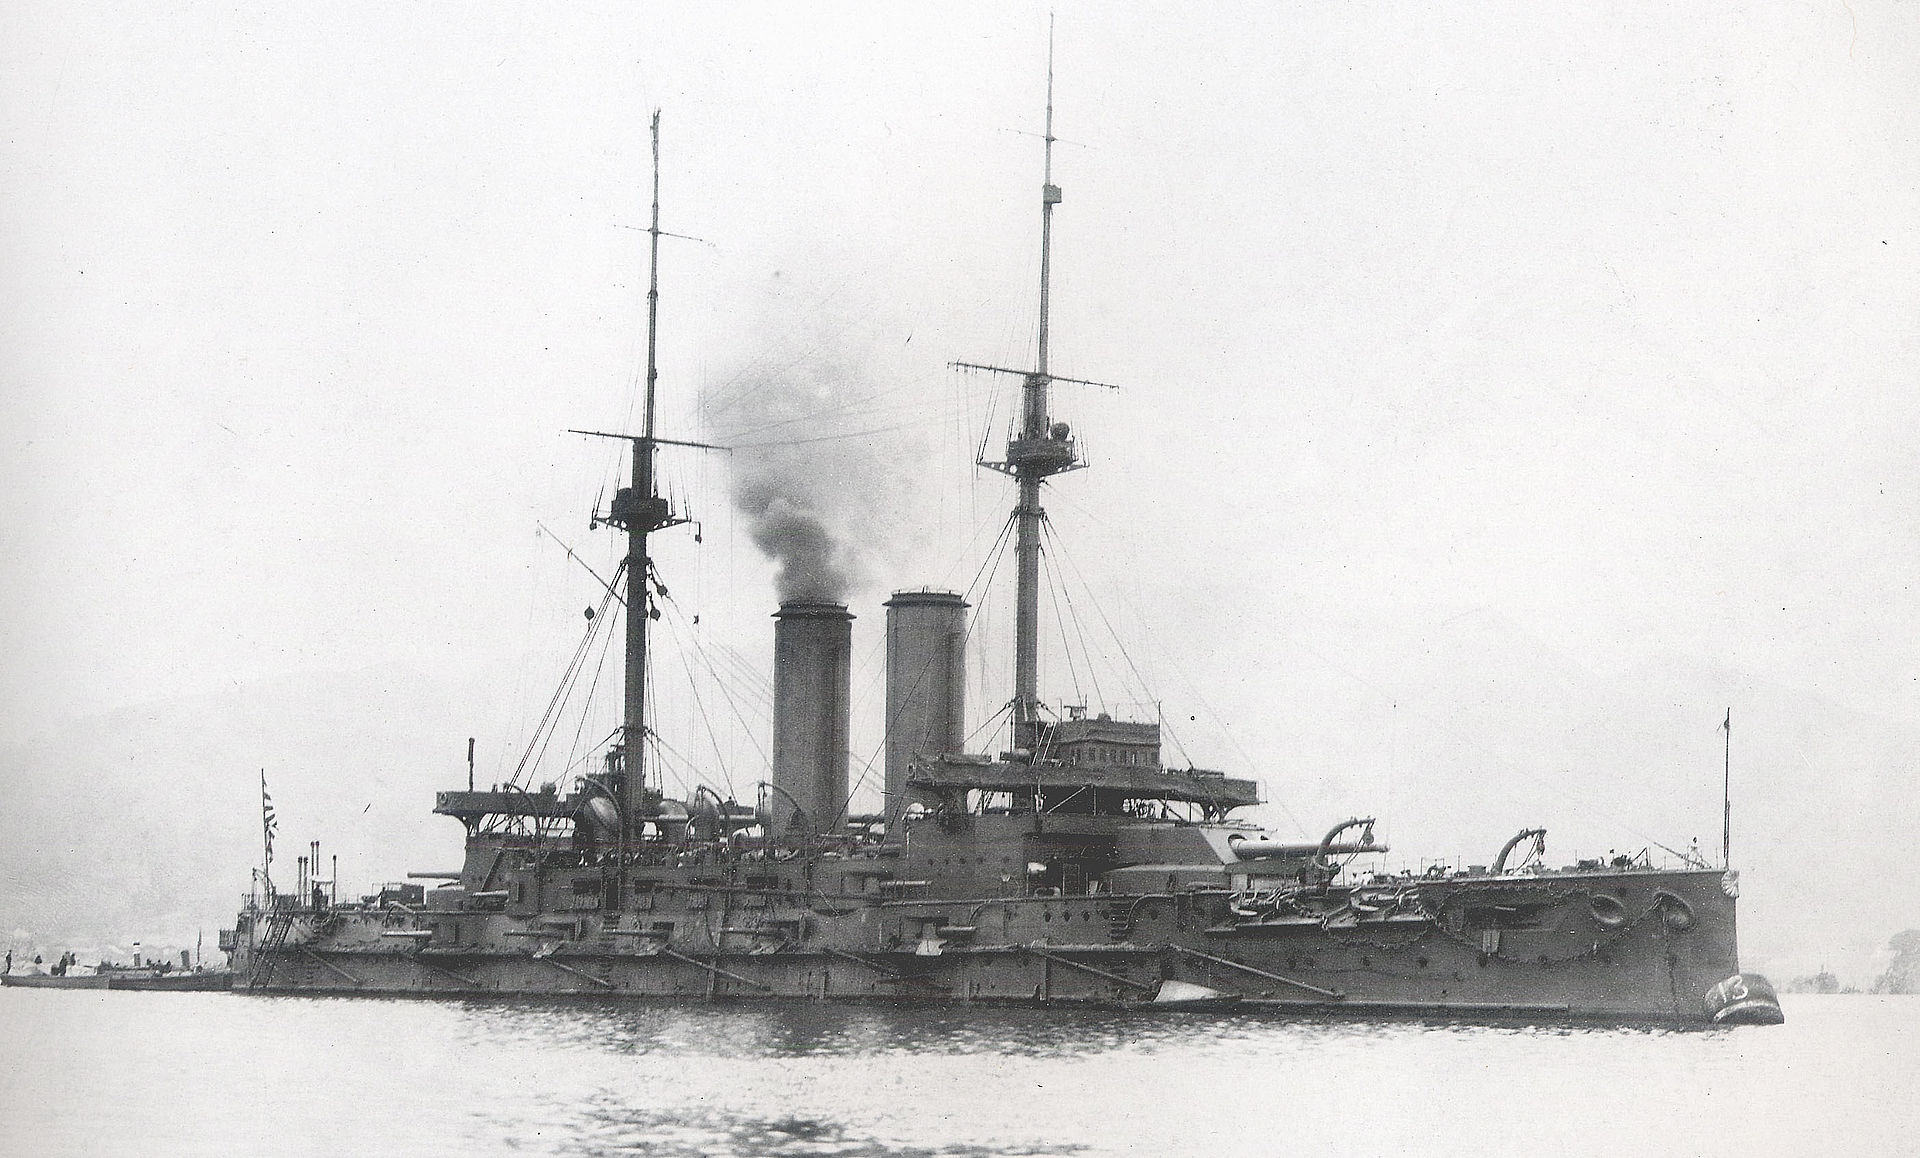
\includegraphics[scale=0.2]{Data/RYAV_sily_storon/A7N2WR2L-TY.jpg}
	%	\label{fig:scipion} % Unique label used for referencing the figure in-text\end{document}
	%	%\addcontentsline{toc}{figure}{Figure \ref{fig:placeholder}} % Uncomment to add the figure to the table of contents%----------------------------------------------------------------------------------------
	\caption{Микаса. Фото неизвестного автора. Взято с Википедии \url{https://en.wikipedia.org/wiki/Japanese_battleship_Mikasa}
	}
	%	CHAPTER 2
\end{figure}

Тут легко впасть в конспирологию. Для любителей возводить тезисы про “англичанку” в абсолют замечу, что среди Британского руководства велись ожесточенные споры касательно продажи современных кораблей развивающимся странам. При этом, как подчеркивает Мак Нил, для некоторых верфей заграничные заказы были единственным способом остаться на плаву.

Итак, у нас две державы. Первая пытается создать флот самостоятельно. Другая закупает почти полностью за границей. Преимущество должно перейти к первой, время работает на нее. Но вот времени как раз-таки у России не было. Значит, стратегия Японии оказалась верной: победа, в конечном итоге, осталась за ними. (4)

Еще одним причиной грядущего поражения стала дрянная подготовка экипажей. Учения не проводились, тактику не преподавали, артиллерийские стрельбы велись редко. Корабли стояли в доках, матросов порой бессмысленно гоняли. Все это откликнется в грядущих боях.

Русско-японская война оказывалась противостоянием одной лишь части созданного практически своими силами отечественного флота с флотом японским, сконструированным на Западных Верфях.


\section{Армия и инфраструктура}

Говоря о русско-японской войне надо понимать, что велась она не только за тысячи верст от Санкт-Петербурга, но и за сотни верст от границы. Отдаленность Порта-Артура делала коммуникации, по словам Айрапетова, растянутыми и уязвимыми. Транзитных баз не имелось. Единственный док для крупных судов располагался во Владивостоке (у японской империи таковых было четыре).

Условия проживания в Порт-Артуре были очень суровыми: болезни, недостаток воды, проблемы с питанием. Не лучше ситуация была и в Дальнем (ныне – Далянь)

Китайские укрепления в Порт-Артуре не годились даже для защиты от каких-нибудь древних кочевников. Было начато строительство фортификационных сооружений. К началу войны, пишет Айрапетов, работы закончили только половину. О том, как это сказалось на обороне, будет сказано в следующих статьях.
Русская армия насчитывала около 1350 тысяч человек и еще 3 с половиной миллиона имелось в резерве.

Оценки японской армии расходятся. Изначально РИ оценивала силы противника в 358 тыс. чел., из них 217 тыс. резервистов. Также предполагалось, что корпус Японии на континенте не превысит 250 тысяч человек. Такое недооценивание стало критичным: Империя Восходящего Солнца мобилизовала в дальнейшем 1,1 миллион и перебросило на фронт 500 тысяч.

\begin{figure}[h!tb] 
	\centering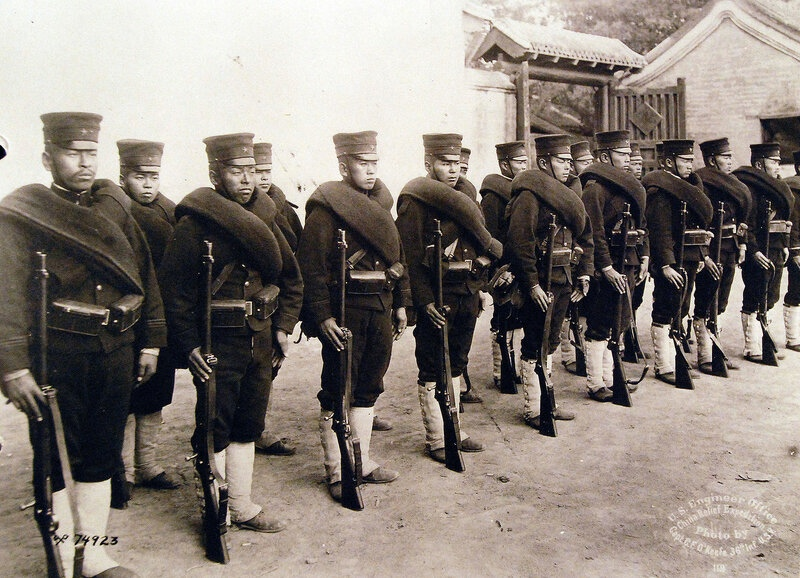
\includegraphics[scale=0.4]{Data/RYAV_sily_storon/kGNdyBmjr4c.jpg}
	%	\label{fig:scipion} % Unique label used for referencing the figure in-text\end{document}
	%	%\addcontentsline{toc}{figure}{Figure \ref{fig:placeholder}} % Uncomment to add the figure to the table of contents%----------------------------------------------------------------------------------------
	\caption{Японская пехота во время Боксерского восстания.  \url{https://477768.livejournal.com/2794115.html}
	}
	%	CHAPTER 2
\end{figure}

На начало войны на Дальнем Востоке русская армия составляла 133 000 человек. Главнокомандующий Куропаткин предполагал постепенное отступление вглубь Маньчжурии, накопление сил, благо Транссиб позволял перебрасывать войска, и контрнаступление, десант в Японии и пленение Микадо. По его расчётам для победы требовалось шесть корпусов. При этом конкретного операций у Куропаткина не имелось, только «общие контуры». Плохое управление оказалось вторым критическим недостатком.

Транссибирская магистраль действительно стала грозным оружием, несмотря на все недостатки. Для переброски армейского корпуса требовалось около 60-70 дней (хотя в теории выходило около 45).

Японская война стала вторым конфликтом после русско-турецкой войны 1877—1878 гг. с применением призывной армией и первой с испытанием массовых резервов. Тут всплыла первая неприятность: основным оружием была новая и еще не освоенная винтовка Мосина, а большинство призывников умели обращаться лишь с «Берданками».

Второй ошибкой стало недооценивание пулеметов. «В начале боевых действий на Дальнем Востоке находилась одна пулеметная команда из 8 пулеметов», - пишет Айрапетов. Наверстывать отставание пришлось уже во время войны.

Итак, Российскую империю назвать отсталой нельзя. Тем трагичнее станут такие просчеты, как экономия на учениях, плохое планирование операций. При этом стоит заметить, что время работало на нас и для победы японцам необходимо было действовать в коротком временном окошке.


Автор Виктор Пепелов. Оригинал \url{https://vk.com/wall-162479647_159545}

\#Пепел@catx2

\#Заметка@catx2


\chapter{Была ли Россия отсталой?}

Когда в Российской Империи появились первые пароходы, в Японии царил сёгунат и голод. Когда Россия приступила к созданию броненосного флота, то в Японии только разворачивалась революция Мэйдзи. Почему же Россию считают отсталой? Была ли война проиграна до начала или нет?

Русские создавали флот с нуля дважды. Первый раз – при Петре I, второй раз – в конце XIX в. В первый раз у них было два направления для экспансии и два грозных противника. Во второй раз – соперничество с самыми крупными морскими державами, а еще оборона двух морей и одного океана. Поэтому при оценке сил двух империй речь пойдет, в первую очередь, о кораблях. 

\section{Русский флот: от Крыма до Японии.}

В советской историографии красной нитью шла речь об «отсталости Царской России». При Сталине отношение к отечественной истории отошло от привычного охаивания в духе школы Покровского. Но вот Русско-японскую войну всегда выставляли как образец позора Российской империи и Романовых. После СССР появилась прямо противоположная точка зрения. Так где же истина?

Вторая половина XIX в. – это время индустриализации военного комплекса. Крымская война была последним крупным конфликтом с применением парусного флота (2). После нее стало ясно: главную роль играют технологии.

\begin{figure}[h!tb] 
	\centering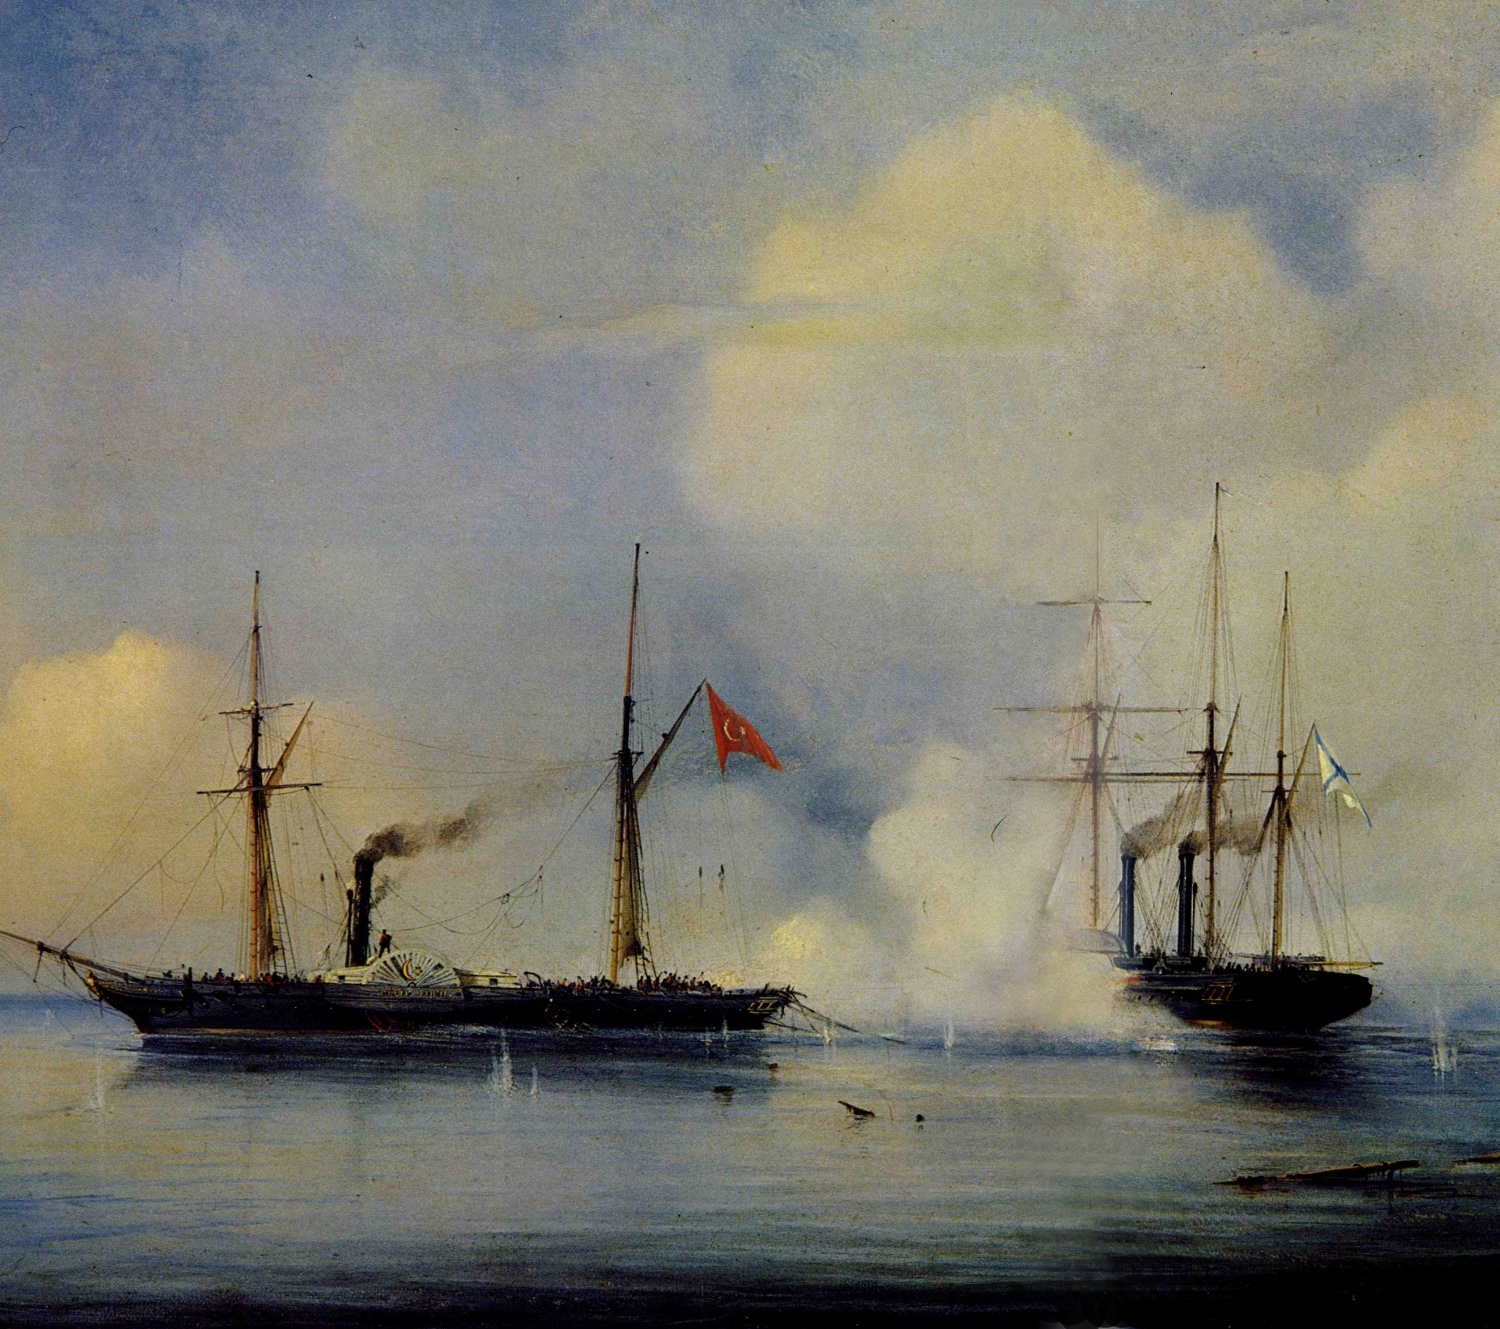
\includegraphics[scale=0.3]{Data/RYAV_sily_storon/rO3nWL7-ijc.jpg}
	%	\label{fig:scipion} % Unique label used for referencing the figure in-text\end{document}
	%	%\addcontentsline{toc}{figure}{Figure \ref{fig:placeholder}} % Uncomment to add the figure to the table of contents%----------------------------------------------------------------------------------------
	\caption{Бой русского пароходофрегата «Владимир» и турецкого парохода «Перваз-Бахри». Художник А. Боголюбов. Это небольшой бой времен Крымской войны стало первым сражением пароходов в истории человечества.}%	CHAPTER 2
\end{figure}

В конце XIX в. вплоть до начала Первой мировой войны в Европейских державах настал период интенсивного военно-промышленного взаимодействия. Военный историк Мак-Нил датирует его с 1884 по 1914 г. На смену фрегатам с белоснежными парусами пришли огромные плавучие броненосцы из стали, проворные катера и подлодки. Торпеды, радио, системы управления огнем стали залогом победы в морских баталиях.

Технологии развивались стремительно. Стратегическая мысль просто не успевала за ним. Прежде адмиралы и министры понимали с ходу каждую инновацию. Теперь же на диалог с изобретателями уходили дни, а на испытания новинок недели и месяцы учений. «Математическая затруднительность проблемы, совершенно явственно превосходившая уровень знаний большинства людей даже из самого узкого круга посвященных, лишала политику минимальной рациональности», – так описывает Мак Нил ситуацию перед Первой Мировой Войной. Эти слова верны и для предшествующих десятилетий.




Назвать Россию отсталой страной сложно хотя бы из-за того, что модернизация флота началась сразу после Крымской Войны. Но и впадать в идеализацию не стоит: завязанная на государство экономика, крепостничество, отсутствие многих отраслей стали препятствиями для создания стальных кораблей. (3)
Не лишним при описании истории Русского флота будет и слово «Геополитика». Кто сильнее: Слон или Кит? Все зависит от среды. Россия не была первой на море, но показала себя неплохой на суше, потопив Наполеона в бескрайних пространствах Восточно-европейской равнины и подплывая через Хартленд Средней Азии к Индии.


Поэтому после Крымской войны о лидерстве на море речь не шла.
\begin{textcitation}
{	
		«Смирившись с невозможностью создать в ближайшее время боевой потенциал флота, равный боевым потенциалам флотов Англии и Франции, и в то же время не желая терять престижа России как одной из крупных морских держав, царское правительство при определении программы нового судостроения исходило из того, что «Россия должна быть первоклассною морскою державою, занимать в Европе третье место по силе флота после Англии и Франции и должна быть сильнее союза второстепенных морских держав» (имелись в виду Пруссия, Швеция и Дания. — Авт.)»}
\end{textcitation} 
пишут В. А. Золотарев и И. А. Козлов в«Трех столетиях Российского флота».\url{http://militera.lib.ru/h/zolotarev_kozlov2/11.html}

\begin{figure}[h!tb] 
	\centering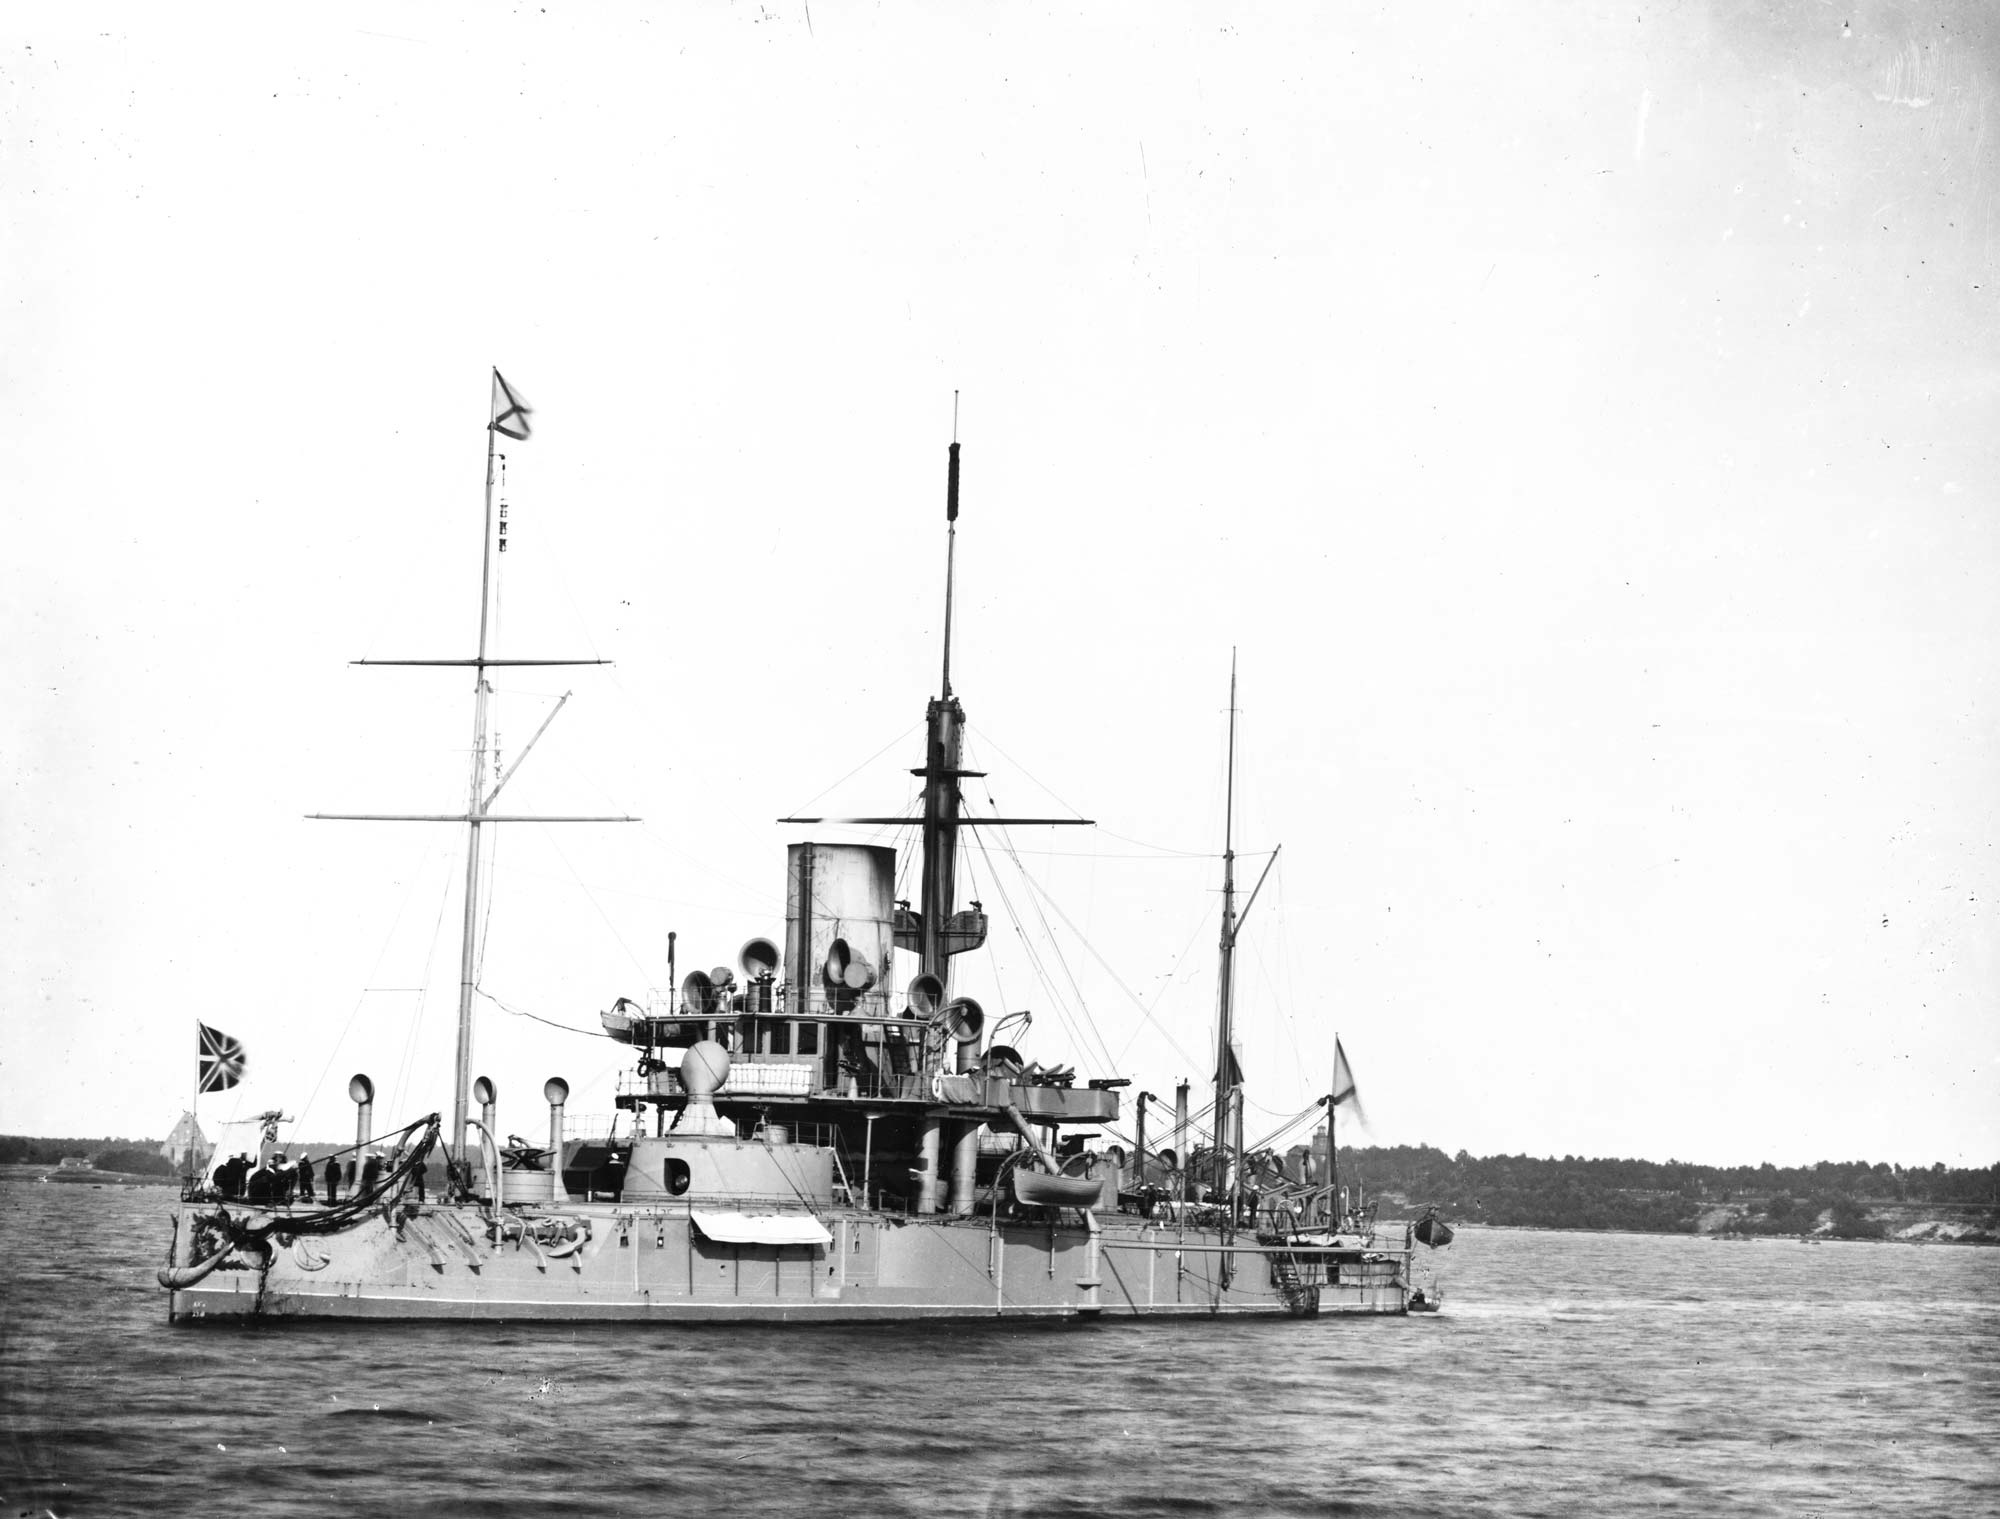
\includegraphics[scale=0.2]{Data/RYAV_sily_storon/jYR7YIwi8uE.jpg}
	%	\label{fig:scipion} % Unique label used for referencing the figure in-text\end{document}
	%	%\addcontentsline{toc}{figure}{Figure \ref{fig:placeholder}} % Uncomment to add the figure to the table of contents%----------------------------------------------------------------------------------------
	\caption{Первый русский броненосец Пётр Великий. Изначально относился к классу Мониторов. Фотографии взяты с сайта «Цусима» \url{http://tsushima.su/petrvelphotoru/} Фото 1}%	CHAPTER 2
\end{figure}


\begin{figure}[h!tb] 
	\centering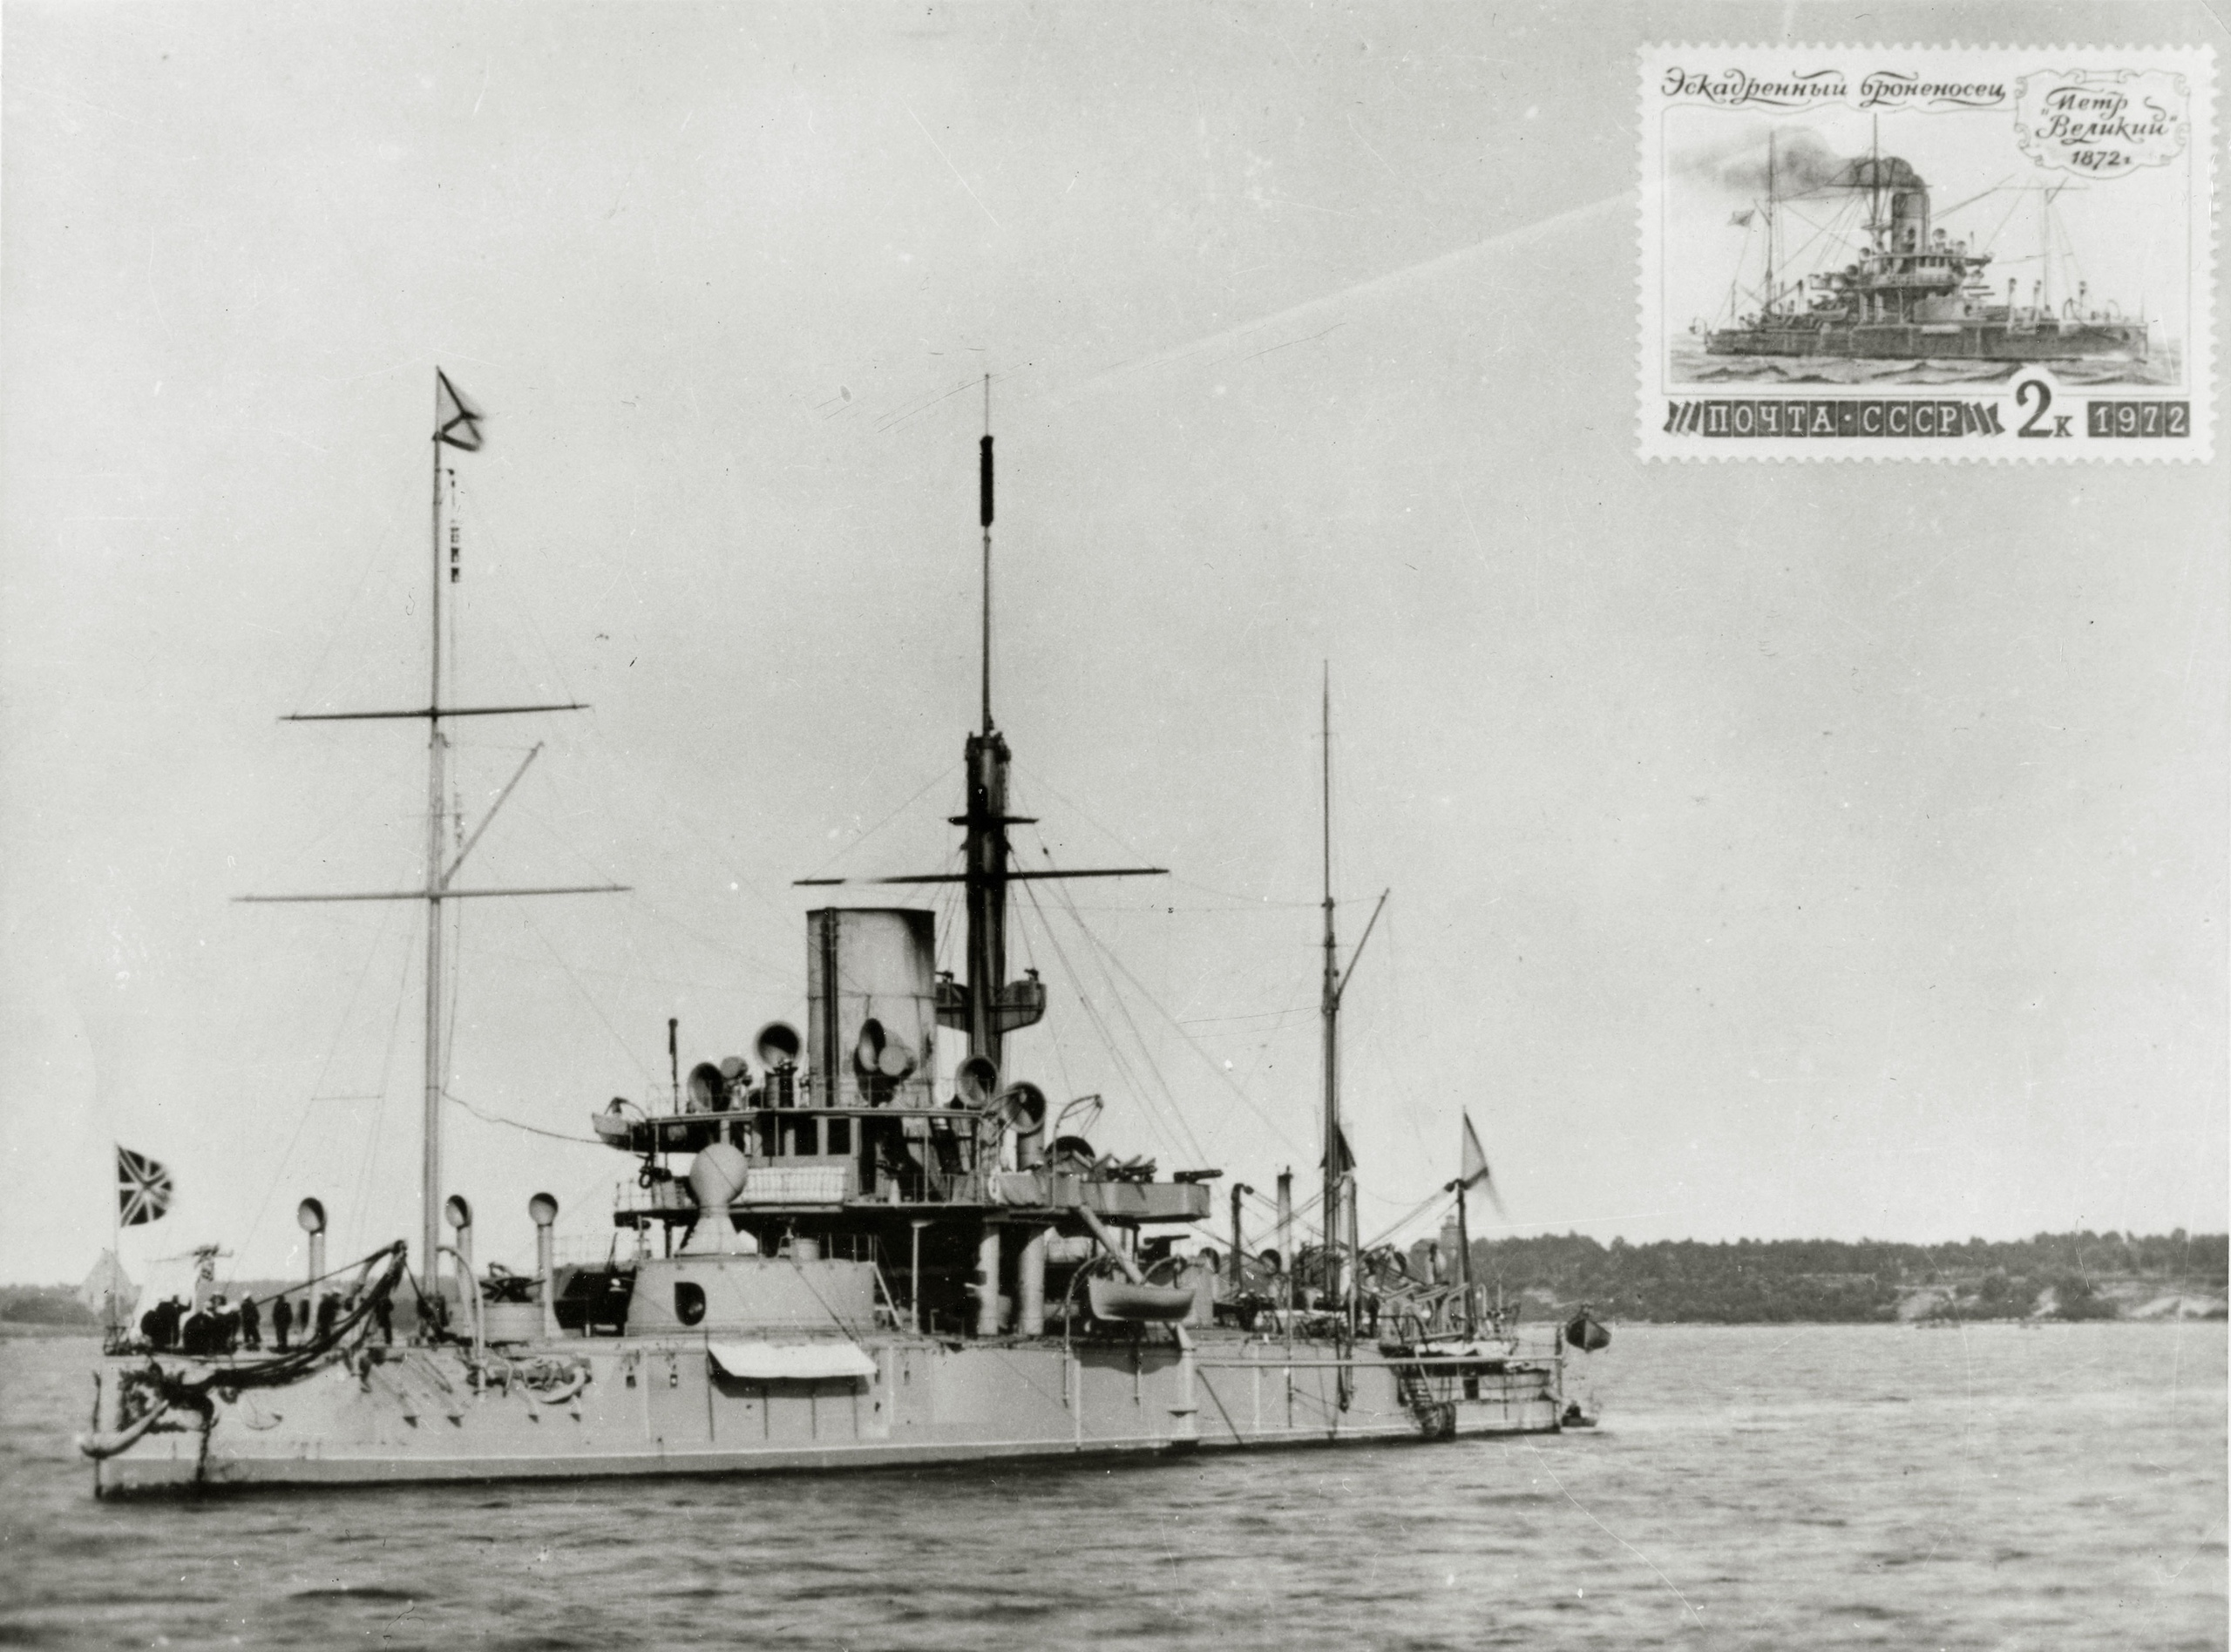
\includegraphics[scale=0.2]{Data/RYAV_sily_storon/wiYS26wh4ZQ.jpg}
	%	\label{fig:scipion} % Unique label used for referencing the figure in-text\end{document}
	%	%\addcontentsline{toc}{figure}{Figure \ref{fig:placeholder}} % Uncomment to add the figure to the table of contents%----------------------------------------------------------------------------------------
	\caption{Первый русский броненосец Пётр Великий. Изначально относился к классу Мониторов. Фотографии взяты с сайта «Цусима» \url{http://tsushima.su/petrvelphotoru/} Фото 2}%	CHAPTER 2
\end{figure}
\begin{figure}[h!tb] 
	\centering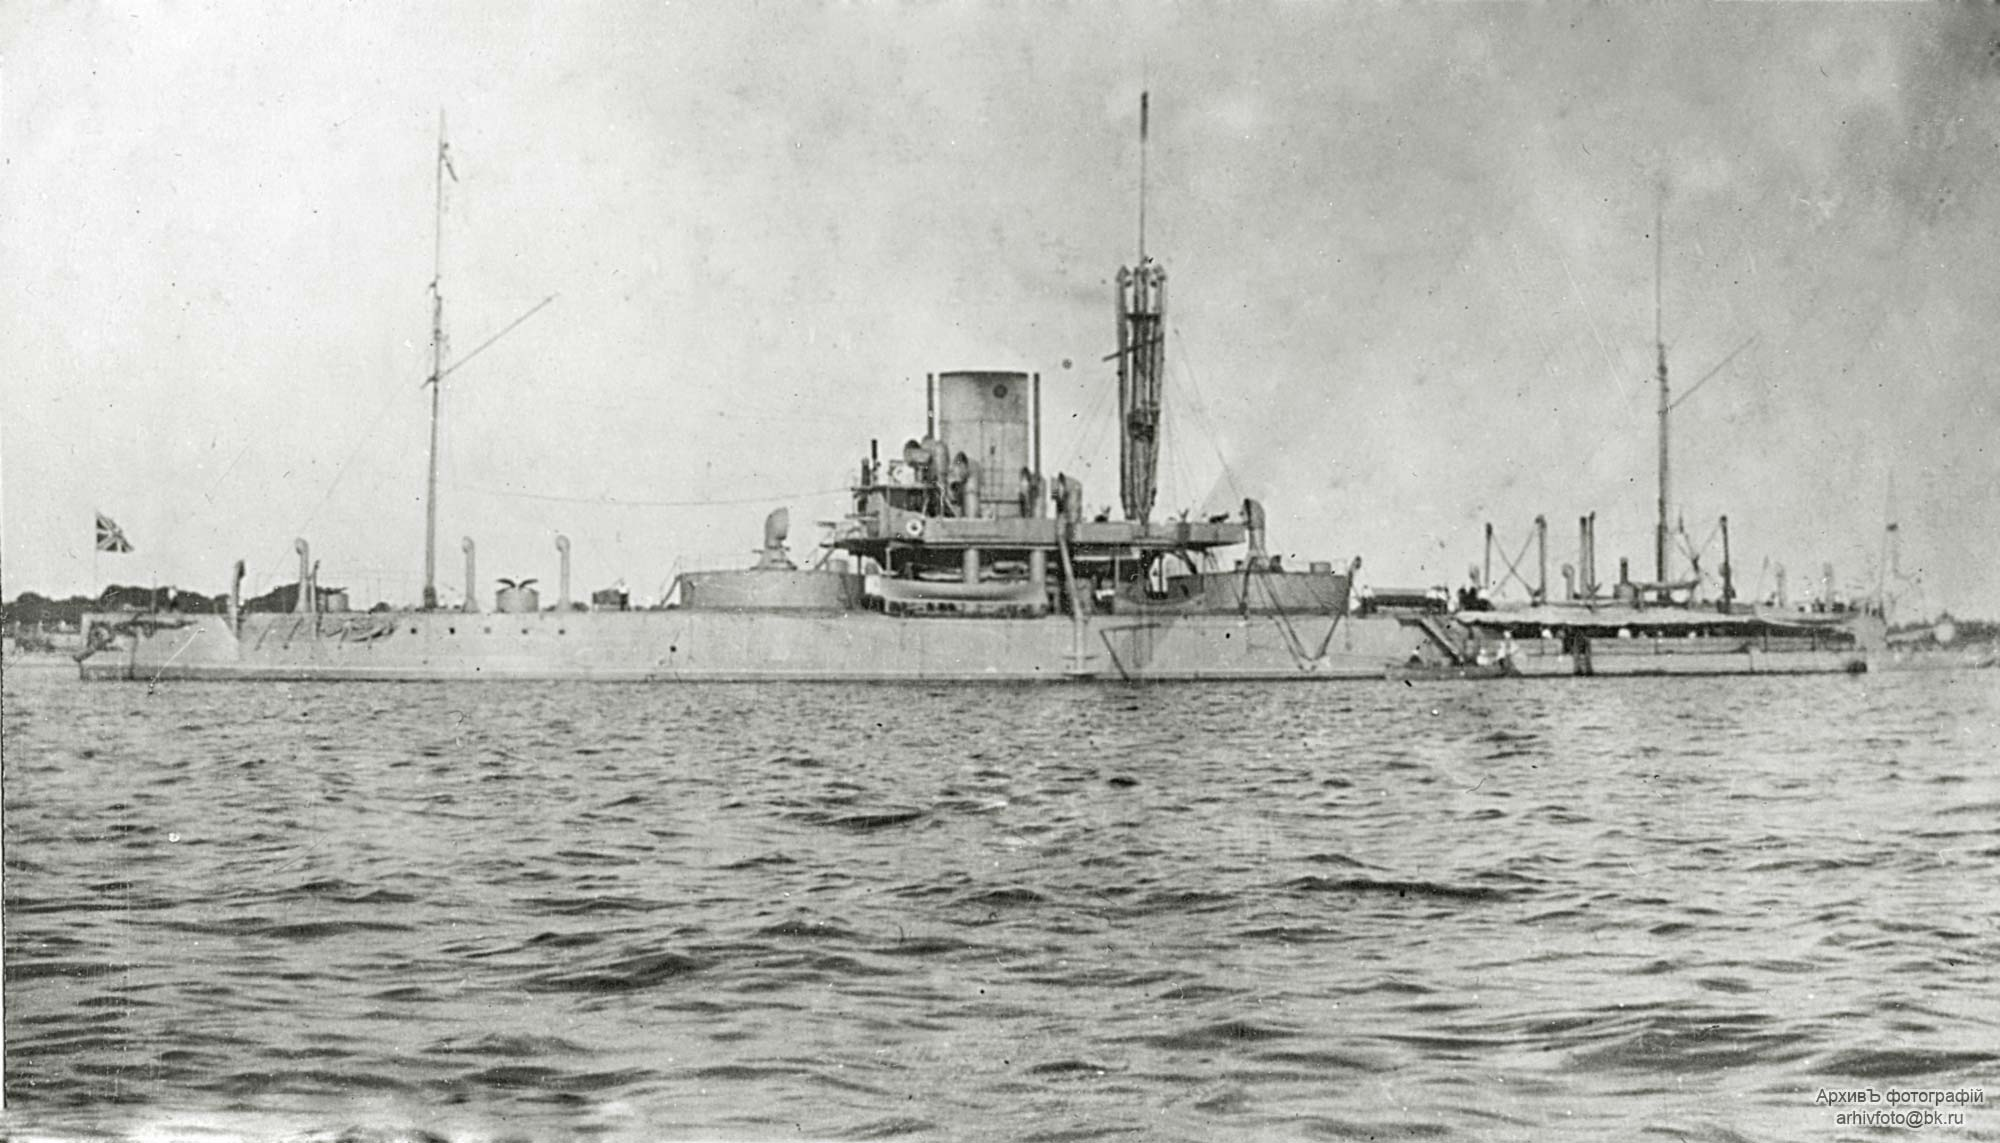
\includegraphics[scale=0.2]{Data/RYAV_sily_storon/dQQjFe6_e2U.jpg}
	%	\label{fig:scipion} % Unique label used for referencing the figure in-text\end{document}
	%	%\addcontentsline{toc}{figure}{Figure \ref{fig:placeholder}} % Uncomment to add the figure to the table of contents%----------------------------------------------------------------------------------------
	\caption{Первый русский броненосец Пётр Великий. Изначально относился к классу Мониторов. Фотографии взяты с сайта «Цусима» \url{http://tsushima.su/petrvelphotoru/} Фото 3}%	CHAPTER 2
\end{figure}

Тем не менее, за 15 лет после Парижского договора на Балтике появился броненосный флот, третий по силе в Европе. Со стапелей сошел и первый полноценный эскадренный броненосец, «Петр Великий». Затем на верфях создали и броненосные крейсеры, быстрые корабли с легкой броней, предназначенные для долгих автономных походов и действий на коммуникациях. Хуже обстояли дела на Черном Море. Южные рубежи решили поначалу охранять «Поповками», огромными круглыми бронированными плавучими крепостями. Они оказались тяжелыми, дорогими и абсолютно бесполезными. Одну такую «тарелку» сделали в Питере и собрали в Николаеве, другую смогли уже построить целиком там. Не всегда развитие технологий идет гладко, как в компьютерной игре от “Парадоксов” или “Цивилизации”. Что и говорить о морской тактике и стратегии. Некоторые светлые умы предлагали даже оснащать корабли таранами и пробивать противника как в античные времена.

\begin{figure}[h!tb] 
	\centering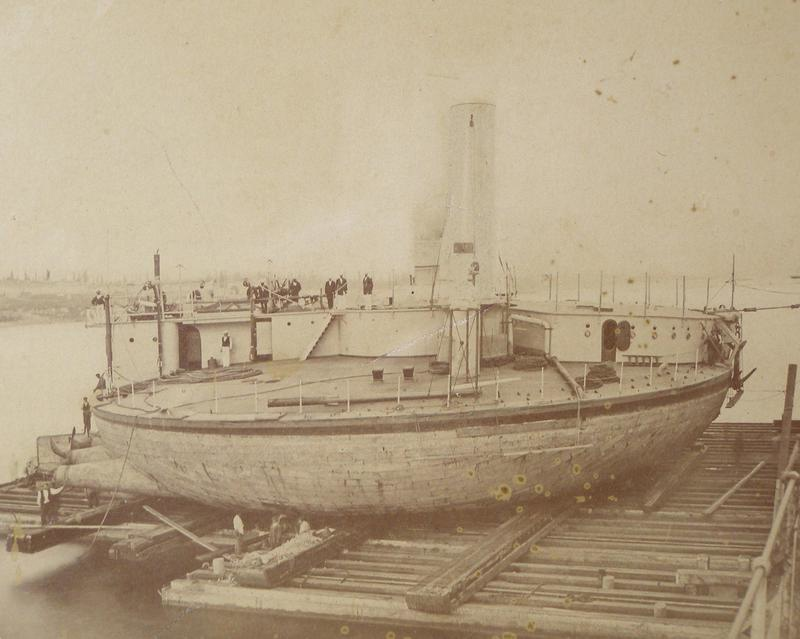
\includegraphics[scale=0.4]{Data/RYAV_sily_storon/GJfhe1Pp85A.jpg}
	%	\label{fig:scipion} % Unique label used for referencing the figure in-text\end{document}
	%	%\addcontentsline{toc}{figure}{Figure \ref{fig:placeholder}} % Uncomment to add the figure to the table of contents%----------------------------------------------------------------------------------------
	\caption{Слабоопознанный плавающий объект «Поповка». Фотография взята с сайта «Поп-механика» \url{https://www.popmech.ru/weapon/13814-plavayushchie-tarelki-absurd/}}%	CHAPTER 2
\end{figure}

В 1880 был принят новый план строительства флота. Мы создавали уже не оборонительно-прибрежный, а океанский. Как видно из таблицы, упор был сделан на Балтику: царское правительство заслуженно опасалось Германской Империи. К тому же Петербург был в то время промышленным центром России.

\begin{figure}[h!tb] 
	\centering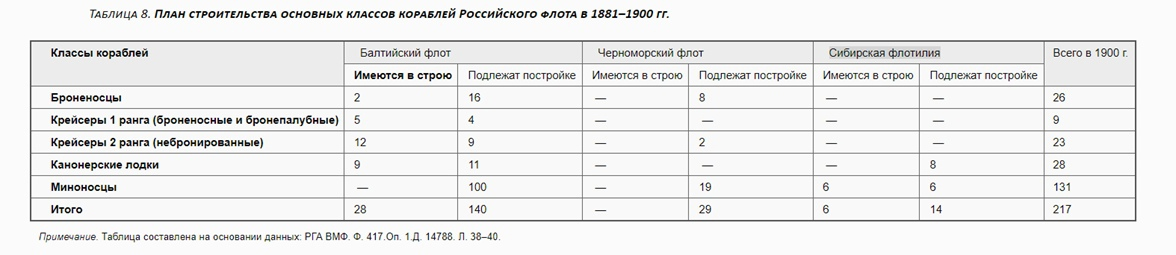
\includegraphics[scale=0.4]{Data/RYAV_sily_storon/eAX9dphs0L4.jpg}
	%	\label{fig:scipion} % Unique label used for referencing the figure in-text\end{document}
	%	%\addcontentsline{toc}{figure}{Figure \ref{fig:placeholder}} % Uncomment to add the figure to the table of contents%----------------------------------------------------------------------------------------
	\caption{Источник: Золотарев В.А., Козлов И.А. Три столетия Российского флота»}%	CHAPTER 2
\end{figure}

В это же время сложилась классификация кораблей флота. Расскажу о ней вкратце (цифры взяты из монографии В. А. Золотарева и И. А. Козлова «Три столетия Российского флота».
1) Эскадренный броненосец или просто броненосец. Огромная плавучая гора с кучей пушек. Минус – неповоротливость. Некоторые же из них, такие как Полтава, еще и не отличались дальностью хода.

\textbf{«Водоизмещение 10–15 тыс. т; вооружение: артиллерийское — четыре 305-мм, до двенадцати 152-мм, до двадцати 75-мм и до тридцати 47–37-мм орудий; торпедное — до четырех надводных и двух подводных торпедных аппаратов; бронирование 406–250 мм; скорость 17–18 узлов; дальность плавания до 8 тыс. миль».}


Первым Броненосцем, если не считать корабль «Петр Первый», был «Император Александр I». Но вплоть до русско-японской войны при постройке вот таких Левиафанов ориентировались на сделанный чуть позже, в 1891 г., «Наварин». В дальнейшем появилось немало броненосцев разных конструкций. Самой многочисленной серией был тип «Бородино».
\begin{textcitation}
«Создание кораблей типа «Бородино» явилось несомненным достижением российской промышленности. Более многочисленные серии броненосцев до этого строились только для британского флота, четыре серии по пять кораблей в каждой в 1895-1907 гг. были построены для флота Германии»,	
\end{textcitation}
подчеркнул Владимир Грибовский про эти суда.\url{http://tsushima.su/RU/libru/i/Page_6/page_15/grib-borodino/}

\begin{figure}[h!tb] 
	\centering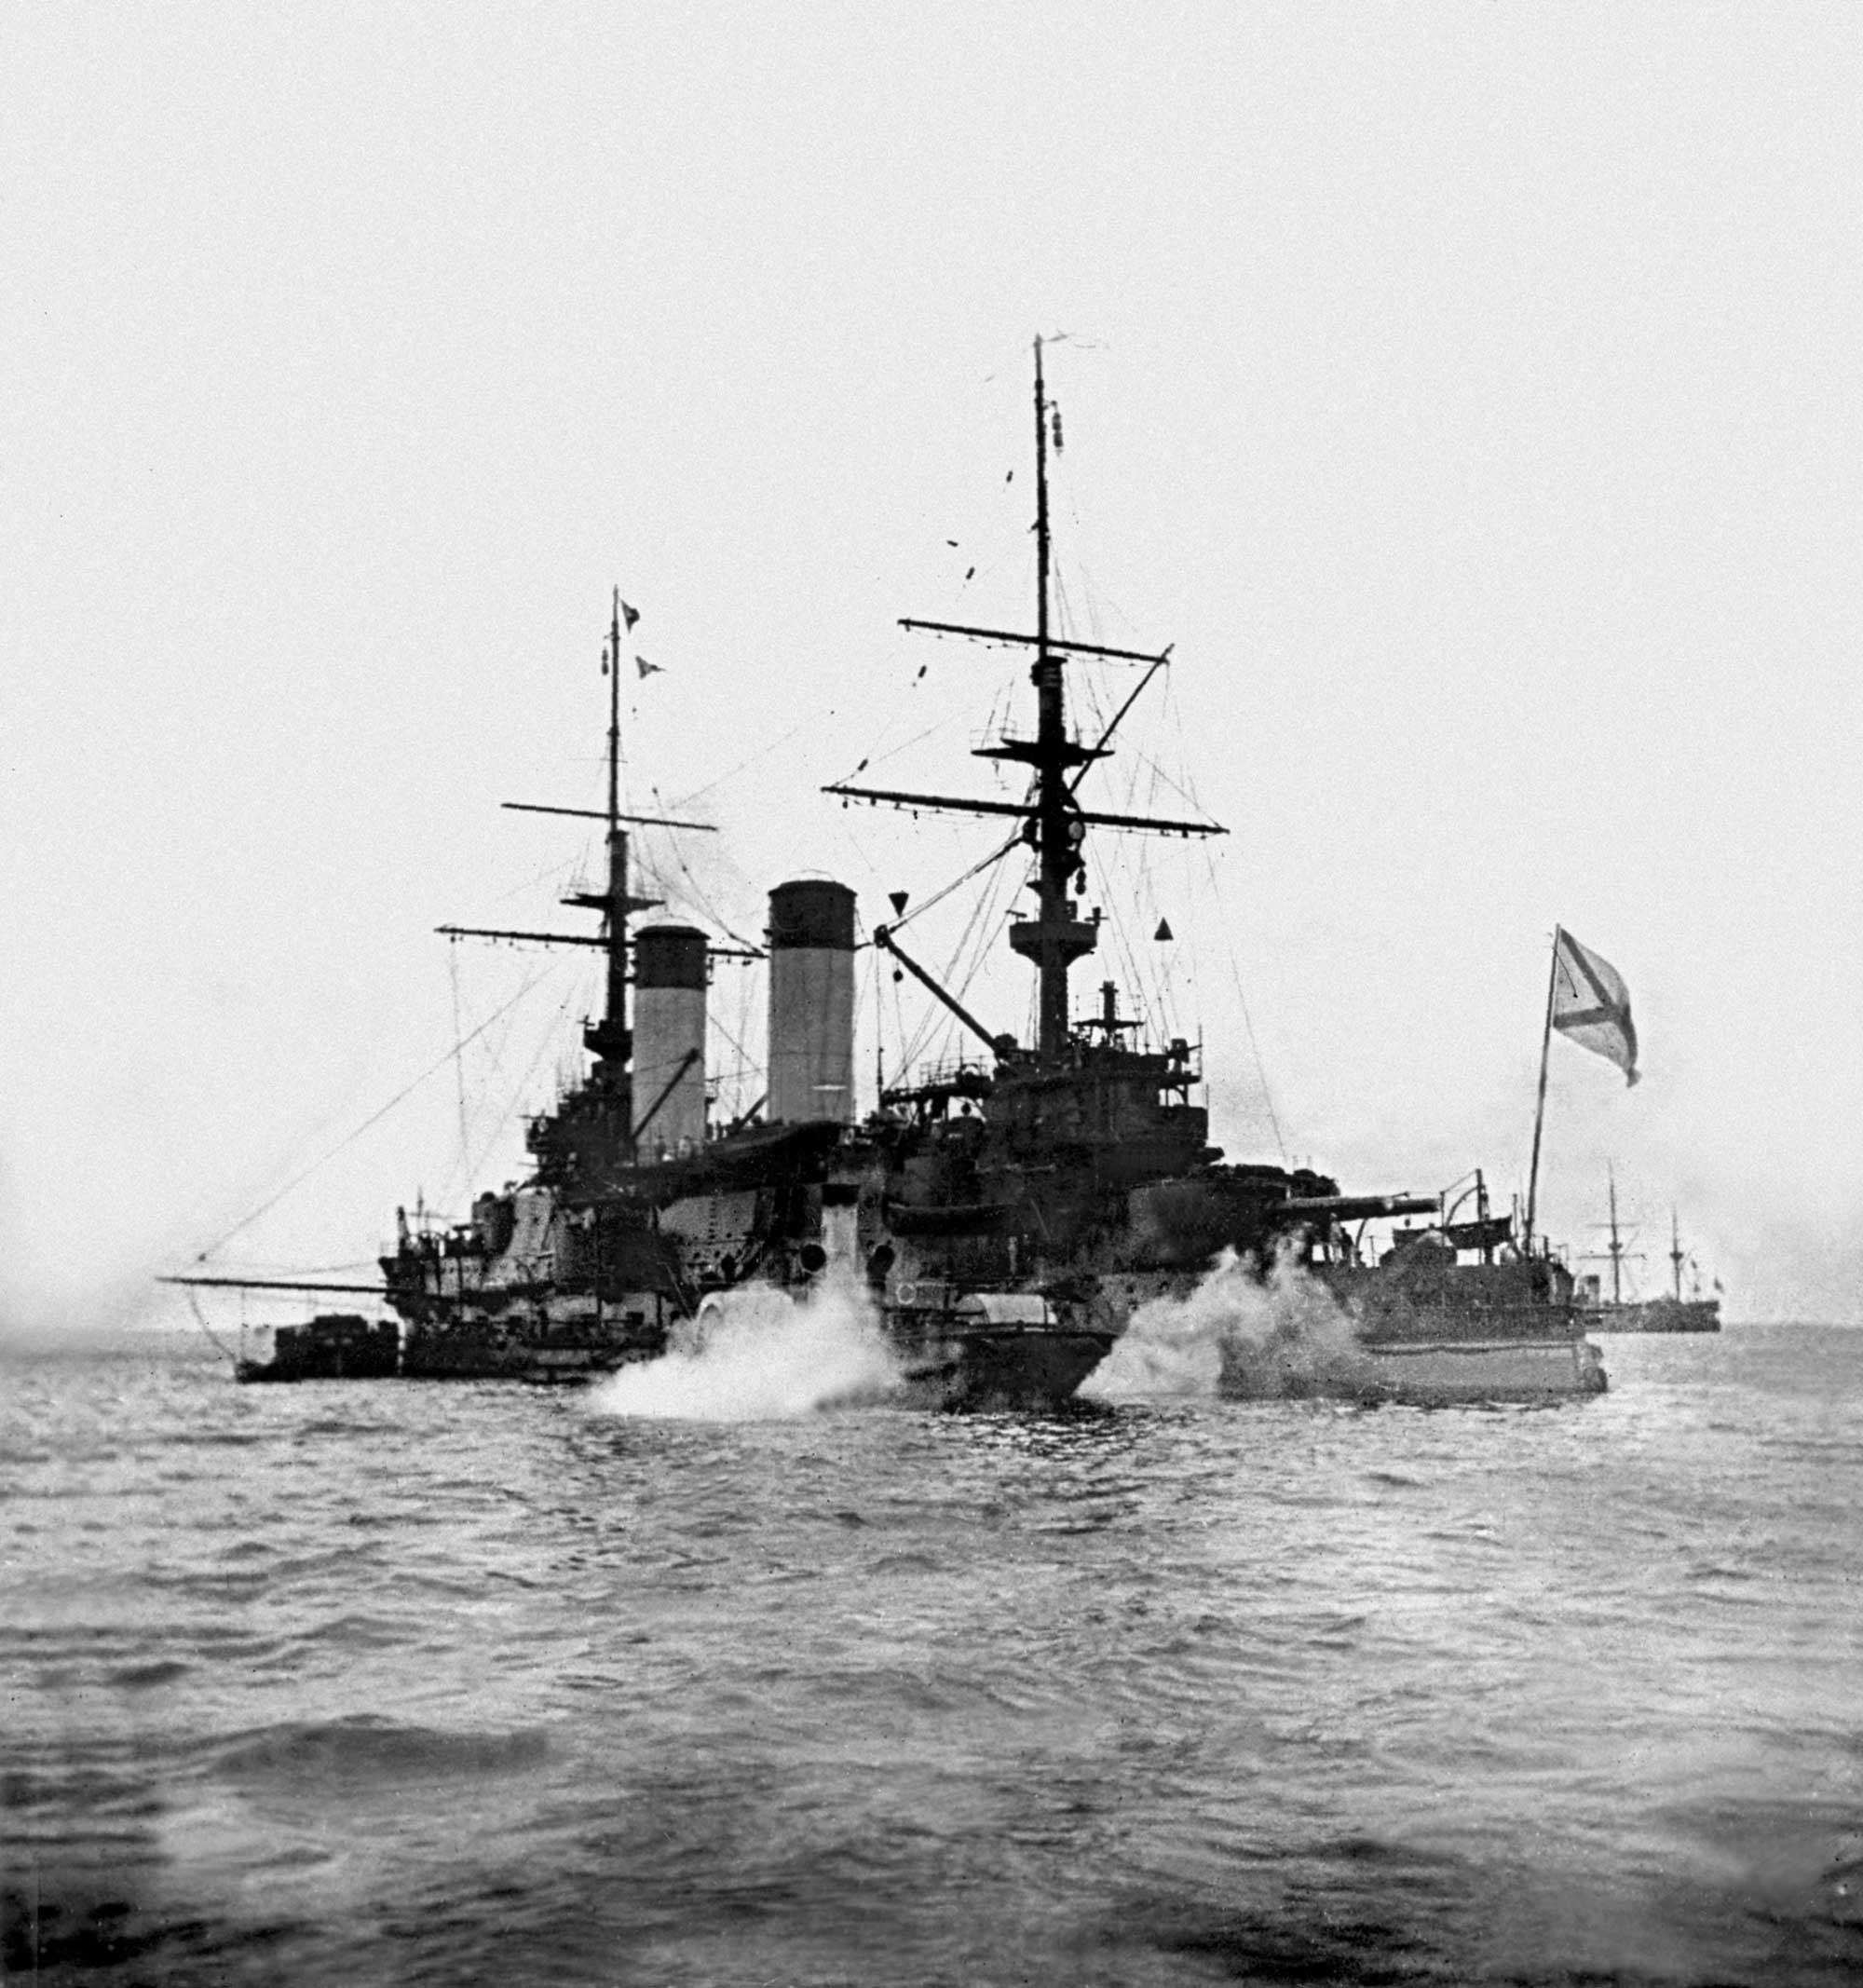
\includegraphics[scale=0.2]{Data/RYAV_sily_storon/pDAKm_tQdIg.jpg}
	%	\label{fig:scipion} % Unique label used for referencing the figure in-text\end{document}
	%	%\addcontentsline{toc}{figure}{Figure \ref{fig:placeholder}} % Uncomment to add the figure to the table of contents%----------------------------------------------------------------------------------------
	\caption{Эскадренный броненосец "Бородино" на малом Кронштадтском рейде. Фотографии взяты с сайта «Цусима»
	}%	CHAPTER 2
\end{figure}


2) Крейсер 1-ого ранга. Проворная плавучая гора с броней, способная как сражаться в эскадре, так и становиться странствующим рыцарем морей, стальной хищной акулой. Самый известный из них – «Аврора» (тип Паллада).

\textbf{«Водоизмещение достигало 12 тыс. т, скорость — 20 узлов, дальность плавания — 8000 миль; вооружение: артиллерийское — четыре 203-мм, шестнадцать 152-мм, до тридцати 37-мм орудий, торпедное — до четырех надводных торпедных аппаратов; бронирование — до 203 мм».}

\begin{figure}[h!tb] 
	\centering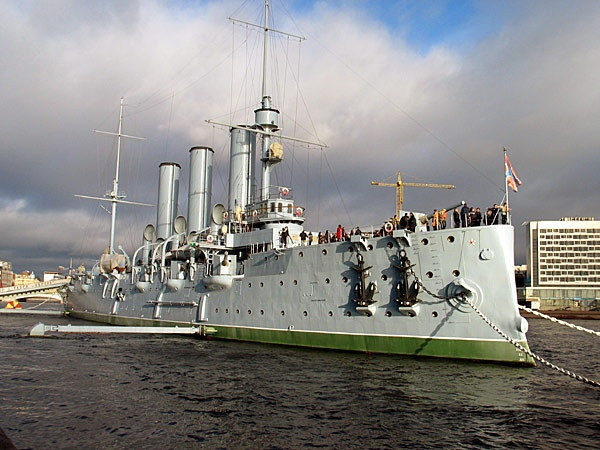
\includegraphics[scale=0.5]{Data/RYAV_sily_storon/o2cXT_E28cA.jpg}
	%	\label{fig:scipion} % Unique label used for referencing the figure in-text\end{document}
	%	%\addcontentsline{toc}{figure}{Figure \ref{fig:placeholder}} % Uncomment to add the figure to the table of contents%----------------------------------------------------------------------------------------
	\caption{«Аврора». Фото с официального сайта \url{http://aurora.org.ru/info/krejser-1-go-ranga-avrora-na-vechnoj-stoyanke-u-petrovskoj-naberezhnoj-sankt-peterburg/}
	}%	CHAPTER 2
\end{figure}

3) Крейсер 2-ого ранга – небольшой корабль для разведки и обороны.

\textbf{«Водоизмещение от 3000 до 6000 т, скорость до 25 узлов, дальность плавания до 4000 миль; вооружение: артиллерийское — восемь 152-мм, двадцать четыре 75-мм, восемь 37-мм орудий; торпедное — до четырех торпедных аппаратов».}

\begin{figure}[h!tb] 
	\centering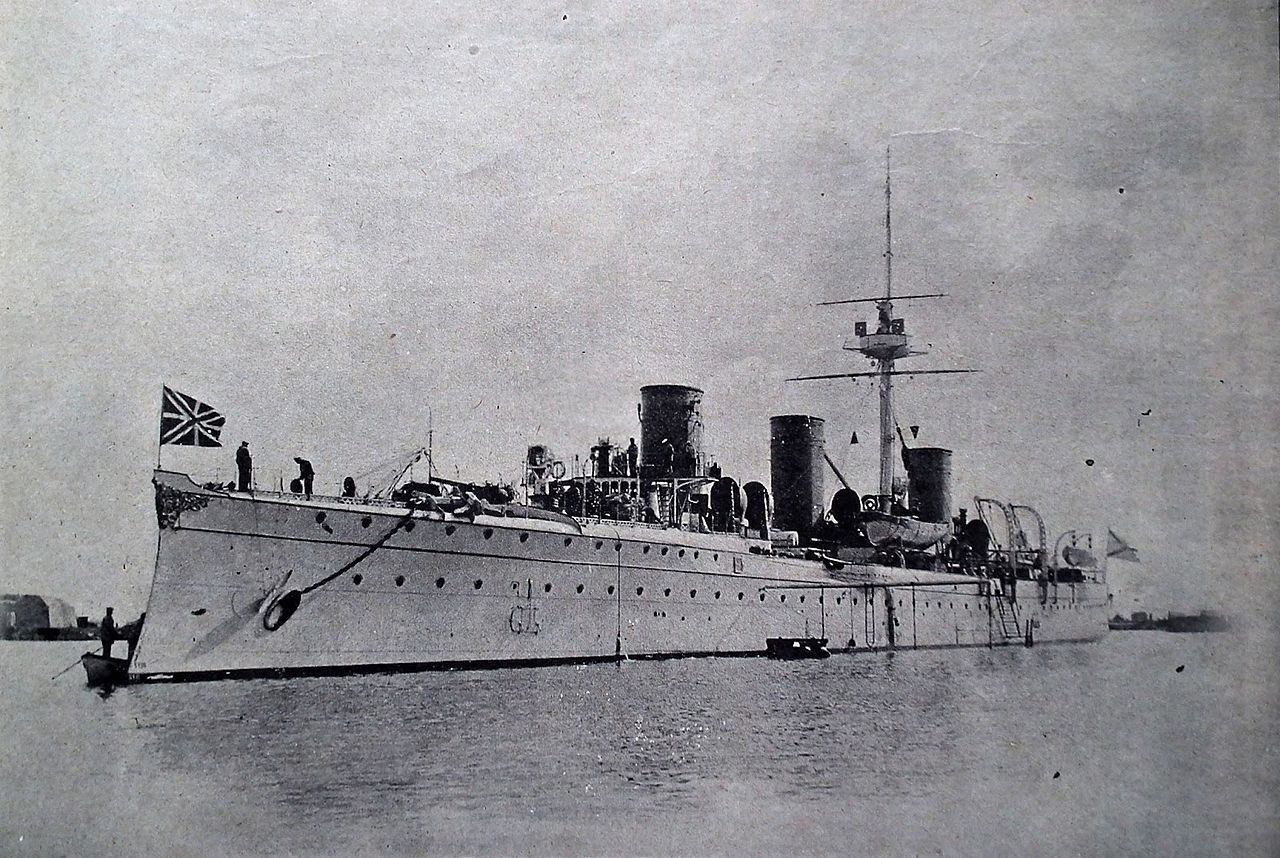
\includegraphics[scale=0.3]{Data/RYAV_sily_storon/f7G2P9E6i0c.jpg}
	%	\label{fig:scipion} % Unique label used for referencing the figure in-text\end{document}
	%	%\addcontentsline{toc}{figure}{Figure \ref{fig:placeholder}} % Uncomment to add the figure to the table of contents%----------------------------------------------------------------------------------------
	\caption{Крейсер II ранга «Новик» }
	%	CHAPTER 2
\end{figure}

4) Канонерская лодка. Небольшое судно, чтоб бить врага вблизи берега.

\textbf{«Водоизмещение до 1500 т, скорость до 15 узлов и по два орудия калибром от 152 до 225 мм».}

\begin{figure}[h!tb] 
	\centering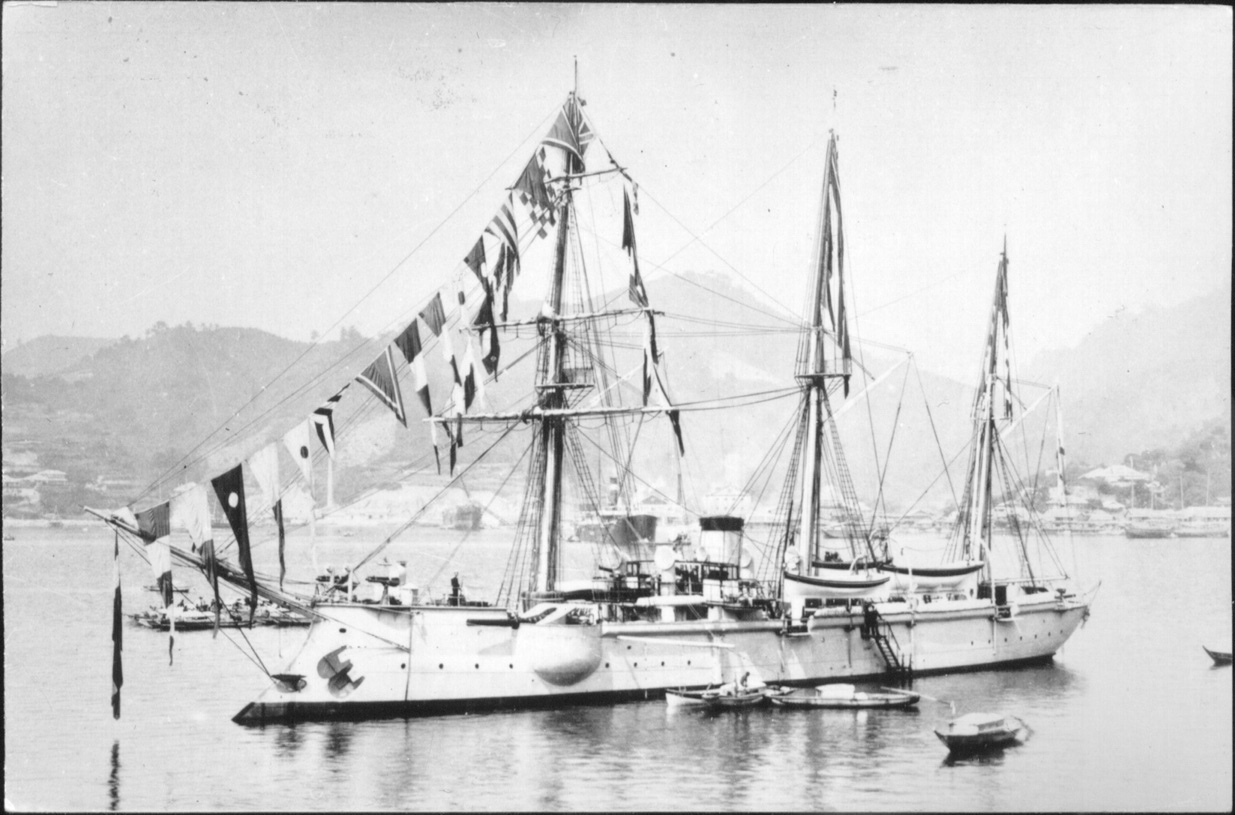
\includegraphics[scale=0.3]{Data/RYAV_sily_storon/7qe4VyVHQn0.jpg}
	%	\label{fig:scipion} % Unique label used for referencing the figure in-text\end{document}
	%	%\addcontentsline{toc}{figure}{Figure \ref{fig:placeholder}} % Uncomment to add the figure to the table of contents%----------------------------------------------------------------------------------------
	\caption{Канонерская лодка «Кореец»
	 }
%	CHAPTER 2
\end{figure}

5) Миноносец и эскадренный миноносец. Маленький, но злой кораблик с торпедами.

\textbf{«Водоизмещение эскадренных миноносцев до 350 т, скорость до 27 узлов, одно 75-мм и пять 47-мм орудий, три торпедных аппарата; у миноносцев водоизмещение до 180 т, скорость до 24 уз., три 37-мм орудия, два торпедных аппарата».}

\begin{figure}[h!tb] 
	\centering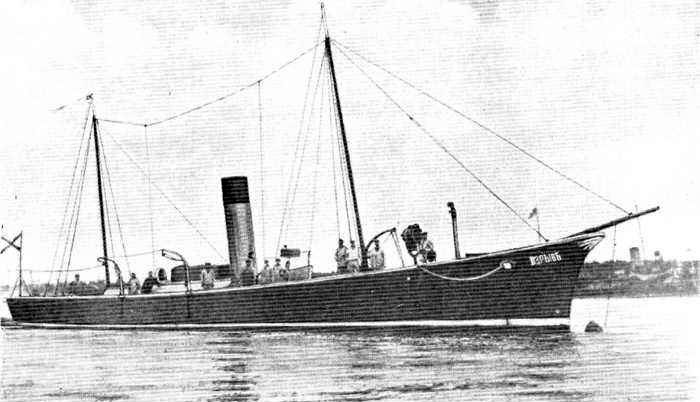
\includegraphics[scale=0.4]{Data/RYAV_sily_storon/a1QM7sSGutc.jpg}
	%	\label{fig:scipion} % Unique label used for referencing the figure in-text\end{document}
	%	%\addcontentsline{toc}{figure}{Figure \ref{fig:placeholder}} % Uncomment to add the figure to the table of contents%----------------------------------------------------------------------------------------
	\caption{Миноносец «Взрыв»
	}
	%	CHAPTER 2
\end{figure}

6) Минный транспорт. Штука, ставящая мины.

\textbf{«Водоизмещение достигало 2800 т, скорость — до 17 узлов, вооружение состояло из пяти 75-мм и семи 47-мм орудий; могли принимать до 300–400 мин».}

\begin{figure}[h!tb] 
	\centering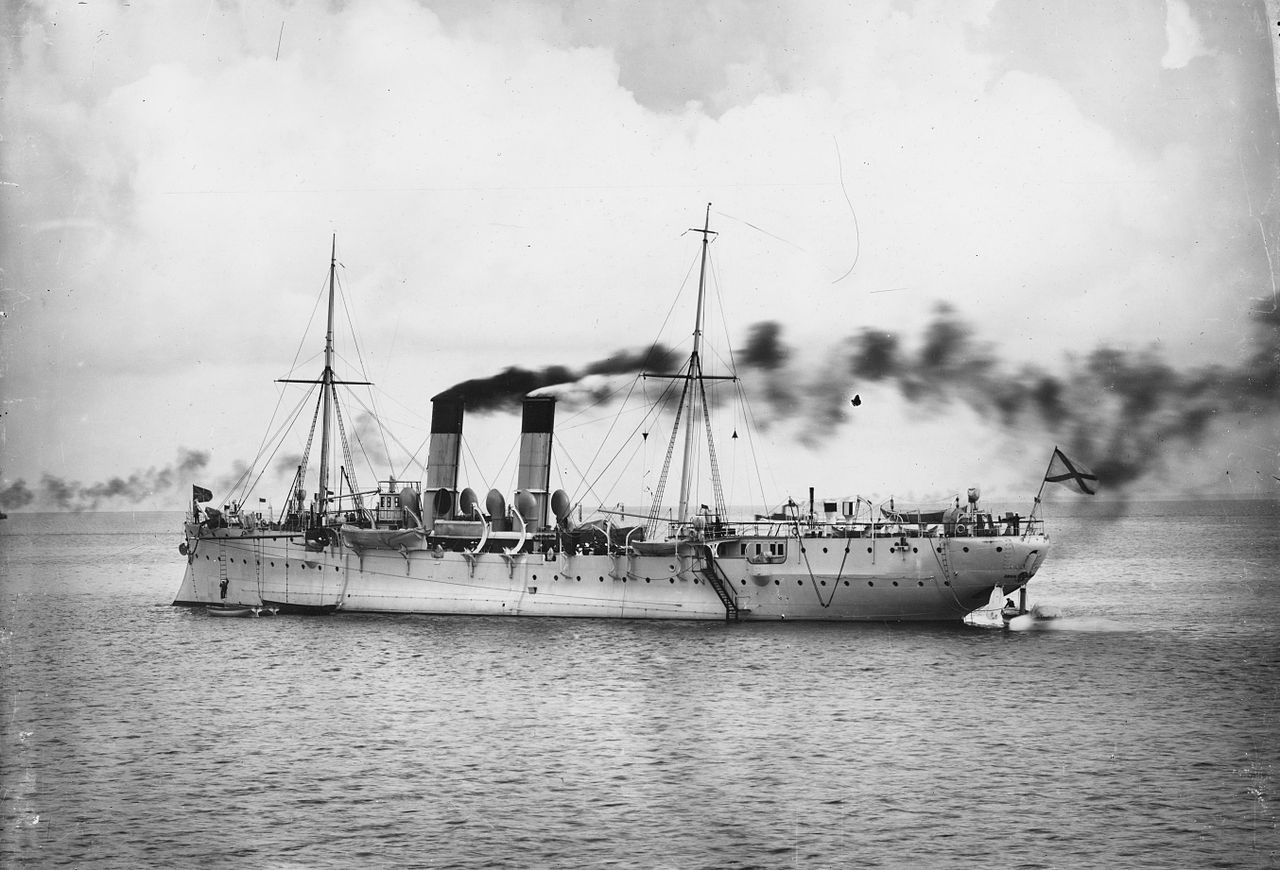
\includegraphics[scale=0.3]{Data/RYAV_sily_storon/w5qmReYSZTc.jpg}
	%	\label{fig:scipion} % Unique label used for referencing the figure in-text\end{document}
	%	%\addcontentsline{toc}{figure}{Figure \ref{fig:placeholder}} % Uncomment to add the figure to the table of contents%----------------------------------------------------------------------------------------
	\caption{Минный заградитель «Амур»
	}
	%	CHAPTER 2
\end{figure}

В 80-х гг начался новый этап строительства флота. В 90-е гг. русский изобретатель А. П. Давыдов создал систему автоматического управления огнем. В тоже время появилась никелированная сталь, радиосвязь и торпеды. «К началу русско-японской войны на вооружении [472] русского флота имелись 45-см торпеды, снабженные гироскопическим прибором управления движением торпеды по направлению, с дальностью хода 2000 м (при скорости 36 узлов) и 1000 м (при скорости 32 узла)».
С другой же стороны, немалая доля «начинки» для тех же кораблей была иностранного производства.
\begin{textcitation}
«При подготовке к походу на «Бородино» были установлены оптические прицелы системы Перепелкина для орудий калибром от 75 до 305 мм, два дальномера системы Барра и Струда, станция беспроволочного телеграфирования системы "Сляби-Арко" германской фирмы "Телефункен", стрелы Темперлея и устройства Спенсера-Миллера для погрузки угля»
\end{textcitation}
 пишет В. Ю. Грибовский в работе об эскадренном броненосце Бородино.

Но такая практика не была редкостью и на Западе. Например, итальянские крейсера типа «Джузеппе Гарибальди» оснащались британской артиллерией фирмы Армстронг. Японские корабли «Касуга» и «Нисима», сделанные на их основе, также несли английские пушки. Работ, подсчитывающих точное соотношение отечественных и западных устройств и оружий, а также технологий, я не нашел.
Благодаря военной реформе Милютина, флот комплектовался не через рекрутские наборы, а ВСЕСОСЛОВНУЮ повинность. Модернизировались и военно-морские училища.
Но почему далеко не худший флот мира проиграл стране, которая в 1850 гг. находилась в состоянии средневековья?

\section{Сравнение Русского и Японского флота}

В целом, русский флот превосходил японский. Но он оказывался распылен на трех направлениях: Тихий Океан, Балтика и Черное море. Проливы и северные воды тревожили Царское правительство, это становится ясно из прошлой статьи про дипломатию. Не выветрилась из памяти и русско-турецкая война 1877-1878 гг.
Но и Дальний восток не уходил из внимания чиновников. Программа по тихоокеанскому флоту была пересмотрена. Готовились резервные эскадры и специальная программа для Дальнего Востока.
\begin{textcitation}
 «Предусматривалось построить (сверх программы 1895 г.) 5 эскадренных броненосцев, 16 крейсеров, 2 минных заградителя и 36 эскадренных миноносцев и миноносцев. Выполнение этой программы должно было закончиться в 1905 г.»
\end{textcitation}
пишут В. А. Золотарев и И. А. Козлов. Именно в это время часть кораблей заказали за границей.
Это привело к тому, что “двуглавый орел” буквально метался с одного конца Евразии на другой. Одни высшие чиновники считали, что приоритет должен остаться за Востоком. Другие, что за Западом.

\begin{textcitation}
«В состав русской эскадры на Тихом океане входили 7 эскадренных броненосцев, 4 броненосных крейсера 1-го ранга, 5 бронепалубных крейсеров 1-го ранга, 2 крейсера 2-го ранга, 6 канонерских лодок, 25 эскадренных миноносцев, 10 миноносцев, 2 минных крейсера, 2 минных заградителя. 1 эскадренный броненосец, 2 крейсера 1-го ранга 1 крейсер 2-го ранга, 7 эскадренных миноносцев, 4 миноносца и 3 транспорта находились в пути на Дальний Восток под командованием вице-адмирала А.А. Вирениуса»
\end{textcitation}
 подытоживает О. Р. Айрапетов.

Против него встал японский флот. 6 новейших эскадренных броненосцев и 6 бронированных крейсеров, т.н. флот «6 на 6». Кроме того, у японцев имелось 6 броненосцев береговой обороны, 7 крейсеров 1-го ранга, 11 крейсеров 2-го ранга, 8 канонерских лодок, 4 минных крейсера и 47 миноносцев. Одновременно, из Средиземного моря в Японию шли 2 броненосных крейсера, купленные в Италии. Таким образом, японцы получили превосходство в ударных силах.

Превосходили ли японские корабли наши? Да.
\begin{textcitation}
 «Три русских броненосца — «Петропавловск», «Севастополь» и «Полтава» являлись уже устаревшими кораблями. <…>. Известный справочник Джейна за 1904 г. соотносил их боевую силу как 0,8 к 1,0 в пользу последних. Кроме того, машины «Севастополя», изготовленные Франко-Русским заводом в Петербурге, отличались низким качеством изготовления и сборки. Даже на официальных испытаниях в 1900 году «Севастополь» не смог развить контрактной скорости (16 узлов), а к началу военных действий с трудом развивал 14» \url{https://cmboat.ru/rusmin1/minonosec3/}
\end{textcitation}
пишет С. В. Несолёный в книге Миноносцы Первой эскадры флота Тихого океана в русско-японской войне (1904-1905 гг.)

И самый главный фактор заключался в том, что Императорский флот Японии превосходил русский в типизации. 
\begin{textcitation}
«Японские эскадренные броненосцы являлись однотипными кораблями новейшей постройки, тогда как русские эскадренные броненосцы, построенные по различным судостроительным программам с интервалом времени до семи лет, принадлежали к четырем различным типам кораблей, обладавшим различными тактико-техническими данными»
\end{textcitation}
продолжает С. В. Несоленый. Да, это не было каким-то сильным превосходством, какое было, например, у регулярной армии над ополчением. Но все равно это дало японцам преимущества. Например, выигрыш в скорости. Русские броненосцы шли медленней на два узла.

При этом японские корабли закупались на Западе. Все броненосцы и практически все броненосные крейсеры сходили на воду с верфей Британии. Большая часть русских судов создавалась – пусть и по западным лекалам – у нас.

И здесь мы отойдем от строго научной литературы в область публицистики. Блогер Половинкин Дмитрий Сергеевич (ЖЖ-юзер Олд-Адмирал) выполнил любительское (но очень качественное) исследование японского флота на основе нескольких научных монографий. Приведу два тезиса.

Японские броненосцы «Сикисима», «Хацусе», «Асахи» и «Микаса» не уступали по своим характеристикам крупнейшим английским кораблям. А вместе эта четверка могла бы набить морду и одному (!) из британских флотов.

Японские броненосные крейсера же имели перекос в сторону боевой мощи, жертвуя остальными параметрами. Такими же характеристиками обладали и вышеупомянутые итальянские корабли Касуга и Нисима. И страна Восходящего Солнца могла себе позволить, так как их противники находились неподалеку. Русские же верфи и промышленные центры располагались на другом конце земного шара. (!)

\begin{textcitation}
«Таким образом, как мы с вами могли убедиться, практически весь японский флот был создан на верфях ведущих кораблестроительных держав. В основном Англии. Выбирались только лучшие проекты и адаптировались под нужные требования. Ядро флота составляли новейшие корабли, характеристики которых в наибольшей степени подходили именно для той войны и того противника, которые выбрала сама Япония. Зачастую это были сильнейшие в мире корабли того времени. Или же превосходство в боевой мощи было достигнуто за счет отказа от тех характеристик, которыми в сложившихся условиях можно было пренебречь» \url{https://oldadmiral.livejournal.com/37890.html}
\end{textcitation}
пишет Олд-Адмирал.

\begin{figure}[h!tb] 
	\centering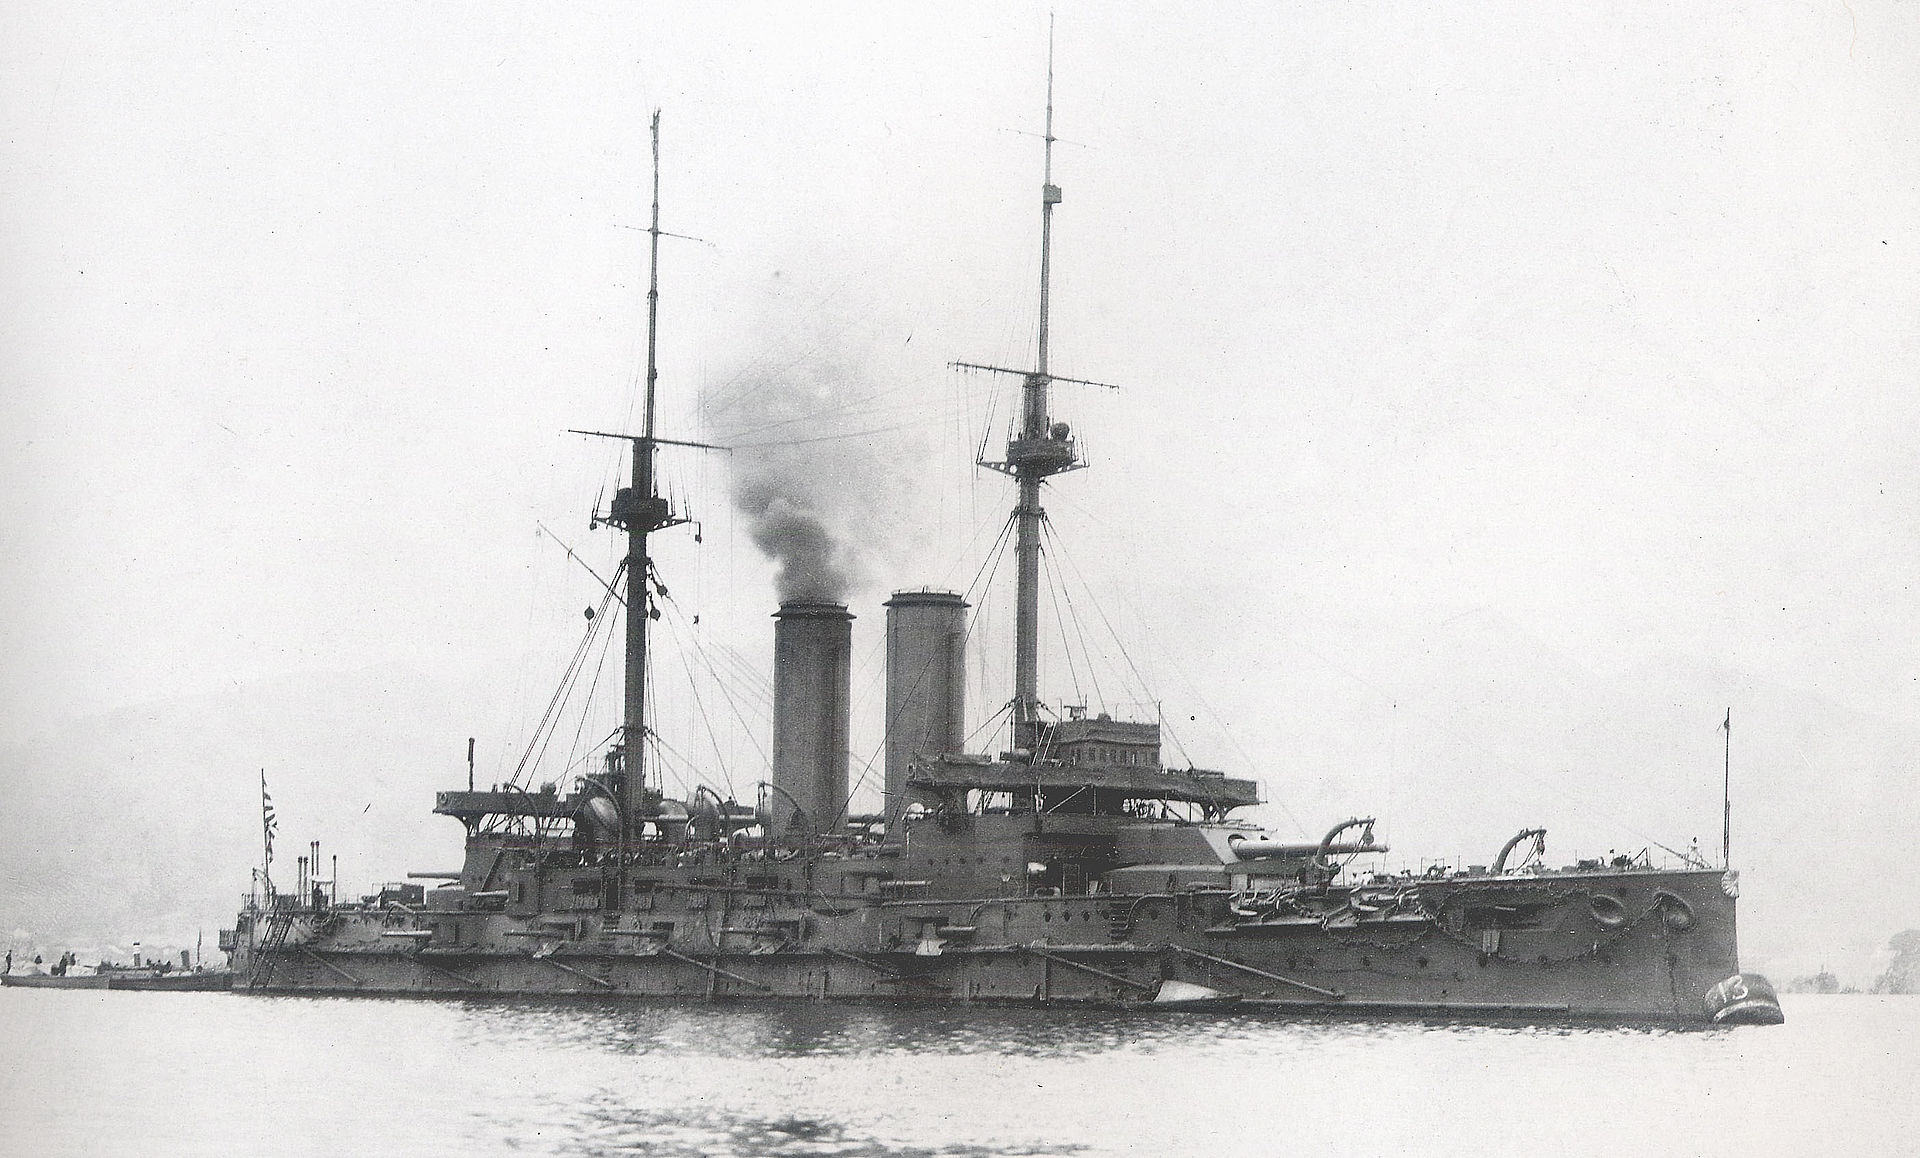
\includegraphics[scale=0.2]{Data/RYAV_sily_storon/A7N2WR2L-TY.jpg}
	%	\label{fig:scipion} % Unique label used for referencing the figure in-text\end{document}
	%	%\addcontentsline{toc}{figure}{Figure \ref{fig:placeholder}} % Uncomment to add the figure to the table of contents%----------------------------------------------------------------------------------------
	\caption{Микаса. Фото неизвестного автора. Взято с Википедии \url{https://en.wikipedia.org/wiki/Japanese_battleship_Mikasa}
	}
	%	CHAPTER 2
\end{figure}

Тут легко впасть в конспирологию. Для любителей возводить тезисы про “англичанку” в абсолют замечу, что среди Британского руководства велись ожесточенные споры касательно продажи современных кораблей развивающимся странам. При этом, как подчеркивает Мак Нил, для некоторых верфей заграничные заказы были единственным способом остаться на плаву.

Итак, у нас две державы. Первая пытается создать флот самостоятельно. Другая закупает почти полностью за границей. Преимущество должно перейти к первой, время работает на нее. Но вот времени как раз-таки у России не было. Значит, стратегия Японии оказалась верной: победа, в конечном итоге, осталась за ними. (4)

Еще одним причиной грядущего поражения стала дрянная подготовка экипажей. Учения не проводились, тактику не преподавали, артиллерийские стрельбы велись редко. Корабли стояли в доках, матросов порой бессмысленно гоняли. Все это откликнется в грядущих боях.

Русско-японская война оказывалась противостоянием одной лишь части созданного практически своими силами отечественного флота с флотом японским, сконструированным на Западных Верфях.


\section{Армия и инфраструктура}

Говоря о русско-японской войне надо понимать, что велась она не только за тысячи верст от Санкт-Петербурга, но и за сотни верст от границы. Отдаленность Порта-Артура делала коммуникации, по словам Айрапетова, растянутыми и уязвимыми. Транзитных баз не имелось. Единственный док для крупных судов располагался во Владивостоке (у японской империи таковых было четыре).

Условия проживания в Порт-Артуре были очень суровыми: болезни, недостаток воды, проблемы с питанием. Не лучше ситуация была и в Дальнем (ныне – Далянь)

Китайские укрепления в Порт-Артуре не годились даже для защиты от каких-нибудь древних кочевников. Было начато строительство фортификационных сооружений. К началу войны, пишет Айрапетов, работы закончили только половину. О том, как это сказалось на обороне, будет сказано в следующих статьях.
Русская армия насчитывала около 1350 тысяч человек и еще 3 с половиной миллиона имелось в резерве.

Оценки японской армии расходятся. Изначально РИ оценивала силы противника в 358 тыс. чел., из них 217 тыс. резервистов. Также предполагалось, что корпус Японии на континенте не превысит 250 тысяч человек. Такое недооценивание стало критичным: Империя Восходящего Солнца мобилизовала в дальнейшем 1,1 миллион и перебросило на фронт 500 тысяч.

\begin{figure}[h!tb] 
	\centering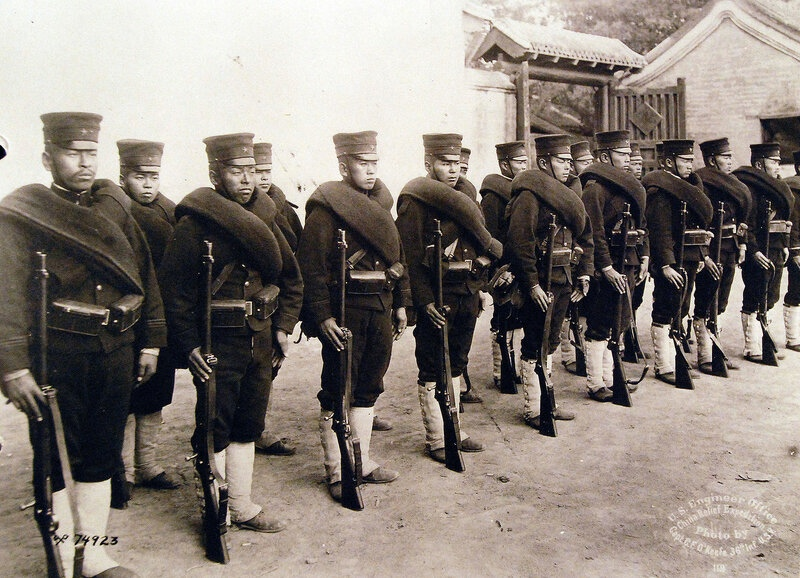
\includegraphics[scale=0.4]{Data/RYAV_sily_storon/kGNdyBmjr4c.jpg}
	%	\label{fig:scipion} % Unique label used for referencing the figure in-text\end{document}
	%	%\addcontentsline{toc}{figure}{Figure \ref{fig:placeholder}} % Uncomment to add the figure to the table of contents%----------------------------------------------------------------------------------------
	\caption{Японская пехота во время Боксерского восстания.  \url{https://477768.livejournal.com/2794115.html}
	}
	%	CHAPTER 2
\end{figure}

На начало войны на Дальнем Востоке русская армия составляла 133 000 человек. Главнокомандующий Куропаткин предполагал постепенное отступление вглубь Маньчжурии, накопление сил, благо Транссиб позволял перебрасывать войска, и контрнаступление, десант в Японии и пленение Микадо. По его расчётам для победы требовалось шесть корпусов. При этом конкретного операций у Куропаткина не имелось, только «общие контуры». Плохое управление оказалось вторым критическим недостатком.

Транссибирская магистраль действительно стала грозным оружием, несмотря на все недостатки. Для переброски армейского корпуса требовалось около 60-70 дней (хотя в теории выходило около 45).

Японская война стала вторым конфликтом после русско-турецкой войны 1877—1878 гг. с применением призывной армией и первой с испытанием массовых резервов. Тут всплыла первая неприятность: основным оружием была новая и еще не освоенная винтовка Мосина, а большинство призывников умели обращаться лишь с «Берданками».

Второй ошибкой стало недооценивание пулеметов. «В начале боевых действий на Дальнем Востоке находилась одна пулеметная команда из 8 пулеметов», - пишет Айрапетов. Наверстывать отставание пришлось уже во время войны.

Итак, Российскую империю назвать отсталой нельзя. Тем трагичнее станут такие просчеты, как экономия на учениях, плохое планирование операций. При этом стоит заметить, что время работало на нас и для победы японцам необходимо было действовать в коротком временном окошке.


Автор Виктор Пепелов. Оригинал \url{https://vk.com/wall-162479647_159545}

\#Пепел@catx2

\#Заметка@catx2

%%%%%%%%%%%%%%%%%%%%%%%%%%%%%%%%%%%%%%%%%%%%%%%%%%%%%%%%%%%%%%%%%%%%%%%%%%%%%
%\printbibliography



\end{document}



